%\documentclass[12pt,draftcls]{ucdavisthesis}
\documentclass[12pt,finalcls]{ucdavisthesis}

% PLEASE READ THE MANUAL - ucdavisthesis.pdf (in the package installation directory)

%%%%%%%%%%%%%%%%%%%%%%%%%%%%%%%%%%%%%%%%%%%%%%%%%%%%%%%%%%%%%%%%%%%%%%%%
%                                                                      %
%               LATEX COMMANDS FOR DOCUMENT SETUP                      %
%                                                                      %
%%%%%%%%%%%%%%%%%%%%%%%%%%%%%%%%%%%%%%%%%%%%%%%%%%%%%%%%%%%%%%%%%%%%%%%%

%\usepackage{bookmark}
\usepackage[us,nodayofweek,12hr]{datetime}
\usepackage{graphicx}
\usepackage{natbib}
\usepackage[titletoc,title]{appendix}
%\usepackage[square,comma,numbers,sort&compress]{natbib}
%\usepackage{hypernat}
% Other useful packages to try
%\usepackage{amsmath}
%\usepackage{amssymb}
%
% Different fonts to try (uncomment only fontenc and one font at a time)
% (you may need to install these first)
%\usepackage[T1]{fontenc} %enable fontenc package if using one of the fonts below
%\usepackage[adobe-utopia]{mathdesign}
%\usepackage{tgschola}
%\usepackage{tgbonum}
%\usepackage{tgpagella}
%\usepackage{tgtermes}
%\usepackage{fourier}
%\usepackage{fouriernc}
%\usepackage{kmath,kerkis}
%\usepackage{kpfonts}
%\usepackage[urw-garamond]{mathdesign}
%\usepackage[bitstream-charter]{mathdesign}
%\usepackage[sc]{mathpazo}
%\usepackage{mathptmx}
%\usepackage[varg]{txfonts}

%% Mike's Packages:

\usepackage[colorlinks=true,linkcolor=blue,citecolor=blue]{hyperref}
\usepackage{amsmath}
\usepackage{amsthm}
\usepackage{amssymb}

\usepackage{eso-pic}
\usepackage{longtable}
\usepackage[width=1\textwidth]{caption}

%\usepackage{tikz}
%\usetikzlibrary{backgrounds,calc}
%\usepackage{media9}
%\usepackage{embedfile}
%\addmediapath{figures}
\usepackage{movie15}
%\usepackage{multimedia}
%\usepackage{tikz}
%\usepackage{placeins}
%\usepackage{marvosym}
%\usepackage[usenames,dvipsnames,table]{xcolor}
%\usepackage{colortbl}
%\usepackage{booktabs}
%\usepackage{graphicx}
%\usepackage{framed}
%\usepackage{setspace}
%\usepackage{xspace}
%\usepackage[labelfont=bf]{caption}
%\usepackage{verbatim}
%\usepackage{paralist}
%\usepackage{algorithm}
%\usepackage{algpseudocode}
%\usepackage{wrapfig}
%\usepackage[font=footnotesize,labelfont=bf,justification=justified,singlelinecheck=false]{caption}
%\usepackage{titlesec}
%\usepackage{natbib}
%\usepackage{longtable}
%\usepackage{tabularx}
%\usepackage{tabulary}
%\usepackage{multirow}
%\usepackage{lipsum}
%\usepackage{mathpazo}
%\usepackage{authblk}
%\usepackage{nameref}
%\usepackage{cancel}
%\usepackage{commath}
%\usepackage{xspace}
%\usepackage{dsfont}
%\usepackage{cuted}
%\usepackage{fancyhdr}

\makeatletter
\newcommand{\chapterauthor}[1]{%
  {\parindent0pt\vspace*{-25pt}%
  \linespread{1.1}\large\scshape#1%
  \par\nobreak\vspace*{35pt}}
  \@afterheading%
}
\makeatother

\makeatletter
\renewcommand\@pnumwidth{1cm}
\makeatother

\newcommand{\opensupplement}{

    \setcounter{figure}{0}

    \renewcommand{\thefigure}{S\thechapter.\arabic{figure}}
}

\newcommand{\closesupplement}{%

        \setcounter{figure}{0}
    \renewcommand{\thefigure}{\thechapter.\arabic{figure}}
     }

\hyphenation{dis-ser-ta-tion blue-print man-u-script pre-par-ing fra-me-work bayes-ian bra-nch} %add hyphenation rules for words TeX doesn't know

%\setlength\overfullrule{5pt}

%\cftsetpnumwidth{3em}

%\renewcommand{\rightmark}{\scriptsize A University of California Davis\ldots \hfill Rev.~\#1.0 \quad Compiled: \currenttime, \today}
% a fancier running header that can be used with draftcls options

%%%%%%%%%%%%%%%%%%%%%%%%%%%%%%%%%%%%%%%%%%%%%%%%%%%%%%%%%%%%%%%%%%%%%%%%
%                                                                      %
%        DOCUMENT SETUP AND INFORMATION FOR PRELIMINARY PAGES          %
%                                                                      %
%%%%%%%%%%%%%%%%%%%%%%%%%%%%%%%%%%%%%%%%%%%%%%%%%%%%%%%%%%%%%%%%%%%%%%%%

\title          {Exploring and Extending Multivariate Brownian Diffusion Models \\of Phenotypic Evolution for Bayesian Phylogenetic Inference}
%Exact title of your thesis. Indicate italics where necessary by underlining or using italics. Please capitalize the first letter of each word that would normally be capitalized in a title.

\author         {Nick Lashinsky}
%Your full name as it appears on University records. Do not use initials.

%\authordegrees  {B.A. (Vanderbilt University) 2013}

\authordegrees  {\phantom{.}}
%Indicate your previous degrees conferred.

\officialmajor  {Anthropology}
%This is your official major as it appears on your University records.

\graduateprogram{Anthropology}
%This is your official graduate program name. Used for UMI abstract.

\degreeyear     {2020}
% Indicate the year in which your degree will be officially conferred.

\degreemonth    {December}
% Indicate the month in which your degree will be officially conferred. Used for UMI abstract.

%\committee{Timothy D. Weaver}{Brian R. Moore}{Shara E. Bailey}{}{}
\committee{Timothy D. Weaver}{Shara E. Bailey}{Peter C. Wainwright}{}{}
% These are your committee members. The command accepts up to five committee members so be sure to have five sets of braces, even if there are empties.

%%%%%%%%%%%%%%%%%%%%%%%%%%%%%%%%%%%%%%%%%%%%%%%%%%%%%%%%%%%%%%%%%%%%%%%%

%\copyrightyear{2020}
%\nocopyright

%%%%%%%%%%%%%%%%%%%%%%%%%%%%%%%%%%%%%%%%%%%%%%%%%%%%%%%%%%%%%%%%%%%%%%%%

%\dedication{\textsl{Dedicated to Pipsqueak \ldots \\
%            Thank you for not dying during my PhD, despite your advanced aged, \\and for joining me in almost every location where non-service animals were welcome.}
%            \AddToShipoutPictureFG*{\put(-15,-27){\includegraphics[width=40mm,scale=1]{figures/pooper.png}}}
%            }

\dedication{\textsl{Dedicated to Pipsqueak \ldots \\
            Thank you for not dying during my PhD, despite your advanced aged, \\and for joining me in almost every location where non-service animals were welcome.}
            }
            
            

%%%%%%%%%%%%%%%%%%%%%%%%%%%%%%%%%%%%%%%%%%%%%%%%%%%%%%%%%%%%%%%%%%%%%%%%

\abstract{Paleontologists and neontologists alike desire improved methods for inferring phylogeny with morphological data, and in this work we hope to not disappoint them too greatly. An introductory section (Chapter \ref{chpt:Chapter1}) surveys our motivations for carrying out this work, and also provides a short overview of continuous character evolutionary models, as well as a short defence of the Bayesian inferential framework. Working in that framework, we explore in Chapter \ref{chpt:Chapter2} the performance of a multivariate Brownian diffusion model (mvBM) at retrieving data-generating tree topologies through an extensive simulation study across a range of idealized and empirically realistic conditions. Following that, we characterize its performance using both standard and novel diagnostic tools, further investigating the extent to which model misspecification of different stripes affects our ability to reliably do phylogenetic inference. Then, we apply this character evolutionary model to two empirical datasets: linear measurements collected from the crania of a globally distributed sample of \textit{Homo sapiens} (Chapter \ref{chpt:Chapter2}), and landmark data collected on the crania of 13 species of catarrhine primate (Chapter \ref{chpt:Chapter3}). The latter are matched to a well-resolved reference tree obtained through analysis of molecular sequence data, and so we compare the performance of our proposed multivariate Brownian model to that of univariate Brownian motion, two discrete character evolutionary models, and a varied set of more commonly used heuristic methods. To explore the nature of inferential errors apparent in this step, we also undertake a study of cranial character evolution using a relaxed morphological clock conditional on the molecular tree, which we then use to parameterize a short simulation study. Finally, in Chapter \ref{chpt:Chapter4} we apply the method to a high-dimensional dataset of discrete dental traits codified using the Arizona State University Dental Anthropology System, assuming a multivariate ordinal probit filter. As joint inference of both phylogeny and tip mean liabilities proved beyond our current computational reach, we adopted two-step approach, first optimizing the locations of tip means, thresholds, and between-trait correlations given individual-level sampling under the multivariate ordinal probit, and then conditioning on these estimates but inferring trait-specific rates in a second, phylogenetic inferential step. To assess the extent to which compromises made in the name of tractability affected our ability to infer phylogeny under this model, we performed a third and final simulation study. In addition, three appendices provide further mathematical details. The first demonstrates how a phylogenetic likelihood under mvBM  --- represented by a high-dimensional multivariate normal density --- can be factored into the product of univariate normal densities. The second describes and validates a novel, tunable proposal distribution over correlation matrices that makes both phylogenetic likelihood calculation and mixing over this especially problematic model parameter much more efficient. The third demonstrates an easy means by which ancestral character states can be sampled from the conditional multivariate normal distribution implied by their location in a tree in conjunction with the data observed at the tree's tips. The dissertation concludes with short section reflecting upon lessons learned and describing directions for possible future work.}

%%%%%%%%%%%%%%%%%%%%%%%%%%%%%%%%%%%%%%%%%%%%%%%%%%%%%%%%%%%%%%%%%%%%%%%%

\acknowledgments{I owe a tremendous debt of gratitude to many parties ensconced both within and without the walls of the University of California, Davis. 

Acknowledged first are my two mentors at UC-D, Tim Weaver and Brian Moore, whose long discussions --- in offices, living rooms, and pubs --- served as ample fuel to stoke the fires of my own scientific curiosity and dedication, while also providing no small measure of fun and enjoyment. Without their guidance and instruction in matters paleoanthropological and phylogenetic none of these projects would ever have left the ground, and I deeply thank them both for accepting me as their mentee. Alongside Tim and Brian, I'd be remiss not to also credit the Anthropology Department and Center for Population Biology to which they and I belonged.

Next, I'd like to thank the folks at \textit{Data Science \& Informatics}, and especially Pamela Reynolds, for giving me the space, funds, and guidance to host many workshops, discussion groups, and my Applied Bayesian Statistics Research Cluster. Outside my own groups, I joined several, and so am also grateful for those riveting chats emerging from paleogroup, morphogroup, pythongroup, computational molecular evolution group, machine learning group, and others. 

Many additional faculty and staff aided me on my graduate career, and so also deserve my gratitude. Peter Wainwright, for highly educational walks in forests and along beaches, for ichthyological side-projects and cluster construction services, for accepting Brian's proposal to let me serve as Bodega workshop coordinator, and for serving on both my qualifying exam and dissertation committees. Mark Grote, for reigning in my \textit{ad hoc}, shoot-from-the-hip statistical proclivities, answering hundreds of convoluted, meandering emails, and consulting on projects in fields ranging from transplant immunology to consumer dietary behavior to Bayesian phylogenetics. Nicolas Zwyns and Richard McElreath, for many fun conversations and for serving as excellent instructors during my initial TAships, as well as for freely giving their slides when it came time to teach my own courses. Teresa Steele, not only for many years of advice and insight in zooarchaeology, but also for letting me in to my first full-summer excavation. Shara Bailey, for training me in dental anthropology during my visit to New York, for lending me her data and insight for my third main dissertation chapter, as well as for providing feedback on the broader dissertation and serving on my qualifying exam and dissertation committees. Though not (yet) faculty anywhere, Mike May also deserves special mention, for his wit, wisdom, and phylogenetic expertise, as well as for acting in the unenviable role as the first person I'd typically turn to for brainstorming project ideas / solutions \& for begging for help when things went awry. 

The students I instructed in my human evolutionary biology, human evolution, and primate evolution courses were all a joy to work with and teach. Thank you for putting up with my inane rambling, lame jokes, dated references, confusing labs, harsh exams, and statistical methods and theory. I wish you all the best in your future careers and endeavors!

%Though not quite students, all those who joined me in 

I would not have had nearly as easy a time of it without the generous financial support of several funding bodies, and so would like to thank the National Science Foundation, the University of California, Davis, and the Department of Anthropology for their assistance, along with those who funded my undergraduate education that I need not to worry myself with debts accrued then and there.

My family, both immediate and extended, deserve much of the credit for those developmental process that shaped me into who I am today, and for chatting with me on my daily walks into work. Especially my mom, grandma, and grandpa. The lattermost of which needs to stop making excuses and return to reading his daily readings!

As my students, friends, and colleagues know all too well, a small dog and smaller cat play a big role in my life, and their emotional support and nightly cuddles have been an excellent way to unwind, 5{\small $\bigstar$}, would recommend to friend.

Friends outside Davis who either flew out to visit or go backpacking with me or who hosted me on their couches, in their spare bedrooms, or their empty houses provided vital distractions from the academic world, and I hope that those past habits can continue once more when conditions allow. Those who maintained a regular teleconferencing habit also deserve a shout-out --- thanks for keeping in touch!

All the friends made at Davis and the Mayo Clinic also deserve mention here. Thank you for your friendship and thoughts, our trivia nights at pubs and our board game, video game, and movie nights at houses, the hikes you joined me on, the lengthy, meandering discussions, and the mutual accountability we provided one another in reading groups.

I'd also like to thank the custodial staff at UC-Davis, who kept facilities clean, took out my trash, and always greeted me with a friendly smile and wave. 

Most of all, I'd like to thank my best friend and life partner, Kate Gates. We met a few days into the PhD program, and my life's been immeasurably better since. Thank you for standing as stalwart bulwark against the frustrations of this experience, and tolerating my angry mutterings at non-compliant, non-compiling code (here's looking at you, \LaTeX). Coming home each night to hang out with you, be it in-person or remotely, formed the highlights of most of these days. By far, you're the best thing that's happened to me during this PhD, and I look forward to many more adventures to come. 

}

%%%%%%%%%%%%%%%%%%%%%%%%%%%%%%%%%%%%%%%%%%%%%%%%%%%%%%%%%%%%%%%%%%%%%%%%

% Each chapter can be in its own file for easier editing and brought in with the \include command.
% Then use the \includeonly command to speed compilation when working on a particular chapter.
%%% \includeonly{ucdavisthesis_example_Chap1}

\begin{document}

%\newcommand{\bibfont}{\singlespacing}
% need this command to keep single spacing in the bibliography when using natbib

%\bibliographystyle{unsrtnat}
\bibliographystyle{apalike}
%many other bibliography styles are available (IEEEtran, mla, etc.). Use one appropriate for your field.

\makeintropages %Processes/produces the preliminary pages

\chapter{Introduction}

\label{chpt:Chapter1}

\chapterauthor{Nikolai G. Vetr}

%\AddToShipoutPictureFG*{\put(-15,-27){\includegraphics[width=40mm,scale=1]{figures/pooper.png}}}


\clearpage


\section{The Need for Phylogenetic Models of Morphological Evolution}

Biological variation both in the extant and fossil records is the outcome of a wide array of evolutionary and non-evolutionary processes. Darwin's ``endless forms most beautiful'' \citep{darwinOriginSpeciesMeans1859} emerge proximally from the complex interplay of environment and development, but ultimately owe the bulk of their between-group differences to millions and billions of years of chance intergenerational sampling effects and reproductive asymmetries attributable to the heritable underpinnings of those organisms' morphology, physiology, behavior, biochemistry, and other traits \citep{mayrNewPhilosophyBiology1988}. Coupled with the bifurcating process by which reproductive isolation emerges and permits populations to proceed along independent evolutionary trajectories, we see these forms --- these \textit{species} --- emerge and change, contract and die. By examining that variation and imagining a description of the processes that might have generated it, we can make inference of phenomena beyond the remit of immediate observation and guess at not just the tempo and mode of character evolution driving within-lineage variation, but also the order and timing of splitting events that birthed those series of independent daughter lineages. 

We can represent an estimated history of these splitting events with a tree, be it one of population history (in the case of groups at the sub-specific level) or phylogeny (for group at or above the species level), which can be rooted to specify the order of events through time, or unrooted, as a means of constraining that order. With a mathematical description --- or stochastic model --- of the evolutionary process that changes the states of characters along branches of the tree, we can predict what sorts of observations we might expect to make at the tips of our tree, and explore how varying properties --- parameters --- of our tree and stochastic model might affect the distributions of those predictions. Comparing our real-world observations with the fictitious ones predicted by our model, we can find combinations of parameters more or less consistent with what we observe. The more plausible our data look under some instantiation of our model parameters, the better evidenced we might say those parameters are, allowing us to discriminate between alternative phylogenetic hypotheses. Through straightforward manipulation of the definition of conditional probability, we can combine a function describing the plausibility of our data with one describing the prior probability of our model parameters to strike a compromise between them, learning what probability we should ascribe to different hypotheses after having made our observations \citep{bayesLIIEssaySolving1763}, at least to the extent that we are willing to accept as given the assumptions of our data-generating process.

If our model is a poor representation of the evolutionary processes that give rise to variation, neither plausible nor probable model parameters may be very trustworthy. Tremendous efforts have gone into developing models to describe the evolution of molecular characters, of nucleotides, amino acids, proteins \citep{hollandRiseStatisticalPhylogenetics2013, kapliPhylogeneticTreeBuilding2020}, but comparably little attention has been paid to models of morphological evolution, especially of the hard tissues that preserve especially well in paleontological contexts. And while neontologists make ample use of increasingly sophisticated methods to infer phylogeny among extant taxa, those reliant on morphology must make do with either heuristic methods lacking in flexibility or other desirable properties \citep[e.g. a principled accounting of inferential uncertainty, consistency at the limit of infinite data, etc.]{wrightBayesianAnalysisUsing2014}, or else fit models of character evolution that make uncomfortable assumptions about the nature of morphological evolution \citep[e.g. independence between characters, monomorphism within lineages, etc.]{felsensteinInferringPhylogenies2004}. And where more sophisticated models exist, their implementation might be sufficiently inefficient as to render practical inference a distant pipe dream, so slow as to be called computationally intractable. 

The work presented in this dissertation does not claim much in way of novelty --- the models contained herein have been known for many decades --- but it does develop a few small tricks that make fitting certain stochastic models more practically efficient under the limits of modern computer hardware, as well as a few novel means of visualizing and interpreting those fitted results. In this manner it extends past work \citep[as e.g.][before it]{felsensteinMaximumlikelihoodEstimationEvolutionary1973, felsensteinUsingQuantitativeGenetic2005}, much as past work made more practical previously proposed methods and theory. Likewise, it does not address every complaint in the matter of biological realism levied against popular models of morphological evolution. But it does explore the statistical properties of some of the more satisfying models under consideration, both on their own merits and in comparison to alternatives. Occasionally, it shifts its attentions away from its primary focus, the set of branching events collectively called the phylogenetic tree's \textit{topology}, and towards other aspects of the phylogenetic model, such as variation in evolutionary rates between characters, across lineages, or through time, or reconstructions of character histories, in the case of truncated biogeographic diffusions. Most of its empirical focus lies with extant humans and close relatives for whom phylogenies and population histories are well-resolved, or at least halfway understood, that more experimental inferential methods may be evaluated by reference to molecular expectation. The primary model considered here is that of multivariate Brownian motion (mvBM), acting either on raw or log-transformed character data, on a vector subspace of that data, or on that data after its been passed through an ordinal probit discretization filter. The mvBM model can be derived under quantitative genetics to correspond a broad range of composite evolutionary processes \citep{hansenTranslatingMicroevolutionaryProcess1996}, and it is exceptionally easy to work with, making it an excellent target for exploratory phylogenetic study. An overview of the broader class of evolutionary models to which it belongs, as well as motivations for using this model over others, can be found in the section below.

\clearpage

\section{A Brief Overview of Popular Continuous Character Evolutionary Models}

\subsection{Ornstein-Uhlenbeck Processes}

Brownian motion can be thought of as nested in another, more parameter-rich model of character evolution called the ``Ornstein-Uhlenbeck'' process \citep[OU]{butlerPhylogeneticComparativeAnalysis2004, beaulieuModelingStabilizingSelection2012}. This process resembles Brownian motion, except it incorporates an elastic, centripetal force by which quantitative traits are pulled toward some optimum value $\theta$ with magnitude of pull proportional to their distance from $\theta$ and a “strength of selection” parameter $\alpha$. Where under Brownian motion  the change a trait underwent in a single time step is state-independent, under OU it depends on the current state, such that $X_{t+1}$ = $X_t$ + $\alpha$($\theta$ – X$_t$) + N($\mu$,$\sigma$), or dX$_t$ = -$\alpha$(X$_t$ - $\theta$)dt + $\sigma$dBt \citep{hansenStabilizingSelectionComparative1997}. If X$_t$ is greater than $\theta$, $\alpha$($\theta$ – X$_t$) will be negative and the trait in the next time step will be pulled “downwards” (proportional to the strength of selection coefficient $\alpha$). Conversely, if $X_t$ is less than $\theta$, X will be pulled upwards in the next time step. Brownian motion, then, arises as an Ornstein-Uhlenbeck process where $\alpha$ is 0. Traits are expected to evolve toward the $\theta$ until they reach it, after which they will fluctuate around it without ever straying too far (Figure \ref{fig:OUPonds}a). The larger $\alpha$ is, the faster traits will reach the optimum and the less they will fluctuate around it. A greater variance in the Brownian motion component of the Ornstein-Uhlenbeck process (i.e. a higher $\sigma$), meanwhile, will increase variance among the traits, leading to non-identifiability when trying to infer the values of $\alpha$ and $\sigma$ from tip data, since an increase in one can be largely counteracted by an increase in the other. 
 
Though the Ornstein-Uhlenbeck process does provide a measure of biological realism, it poses certain additional difficulties to the inference of phylogeny itself, difficulties that may render attempts to use it to retrieve model parameters such as tree topology futile. Under univariate OU with a single peak, the distribution of continuous character states at time $t$ for a character with starting value X$_0$ is normal, with mean $\theta + e^{-\alpha t}(X_0 - \theta)$ and variance $\sigma^2(1-e^{(-2\alpha t)} / (2\alpha)$. From this, it is easy to see that as $t$ increases, the expression $e^{-\alpha t}(X_0 - \theta)$ goes to 0, and the long-term behavior of X centers around $\theta$, with variance determined by our two non-identifiable OU model parameters $\alpha$ and $\sigma$. Effectively, this limits the extent to which the signature of shared ancestry can persist in realizations from an OU-process at the tips of a tree. After sufficient time has passed, all tip values sample from the same, independent distribution determined by $\theta$, $\alpha$ and $\sigma$, which is to say there no longer exists information about between-tip character covariation due to shared ancestry in those values. Rather than phylogenetic covariances decreasing linearly with phylogenetic distance, they instead increase exponentially \citep{hansenTranslatingMicroevolutionaryProcess1996}. Conversely, if $\alpha$ or $t$ are sufficiently small, such as when characters are far from their soft limits in state-space over the timescales represented in the phylogeny, the OU process resembles a Brownian motion process, for which there exist more convenient and tractable multivariate likelihood functions as described later in this work (Chapter \ref{chpt:Chapter2} and Appendix \ref{app:App1}). 

To summarize, then: the more a single-peak OU process is needed to describe the character evolutionary process, the less useful realizations from that process will be for phylogenetic inference. For our purposes here, it may be best to first understand the extent to which Brownian motion, in its best-case context of little-to-no model misspecification, performs, leaving for others a greater detail exploration of those contexts in which an OU model breaks down when used to infer phylogeny. Additionally, a single-peak OU process may itself be a poor fit to the data, for which reason we might wish to posit the existence of multiple peaks. But adding peaks also adds parameters whose inference of marginalization is necessary, potentially robbing us of the power necessary to infer phylogeny and complicating our computations greatly. And at the limit, we might wish to specify as many peaks as we have independently evolving lineages, and further relax the assumption that these peaks' locations be static through time, perhaps allowing them to wander themselves in a manner analogous to fluctuating selection. But such a complex model strongly resembles a laggy Brownian motion, and indeed collapses to Brownian motion at sufficiently high $\alpha$ \citep{hansenTranslatingMicroevolutionaryProcess1996}. Similarly, uncorrelated selection models (where the magnitude and direction of selective effects are sampled from some background distribution, typically normal, across time steps) and directional selection models (where all lineages share the same selective pressures) can also be shown to be equivalent to a Brownian motion model under certain conditions \citep{hansenTranslatingMicroevolutionaryProcess1996}.

This is not to say that OU-models are not useful, especially within their more usual role, serving as a candidate model in the phylogenetic comparative method. In work done in association with this dissertation but outside its scope, I explored their application in Stan for predicting reactive nitrogen concentrations across a hierarchically structured set of manure ponds across California (Figure \ref{fig:OUPonds}). But their use here is limited, and so they shall not be considered further.

\begin{figure*}[h]
\centering
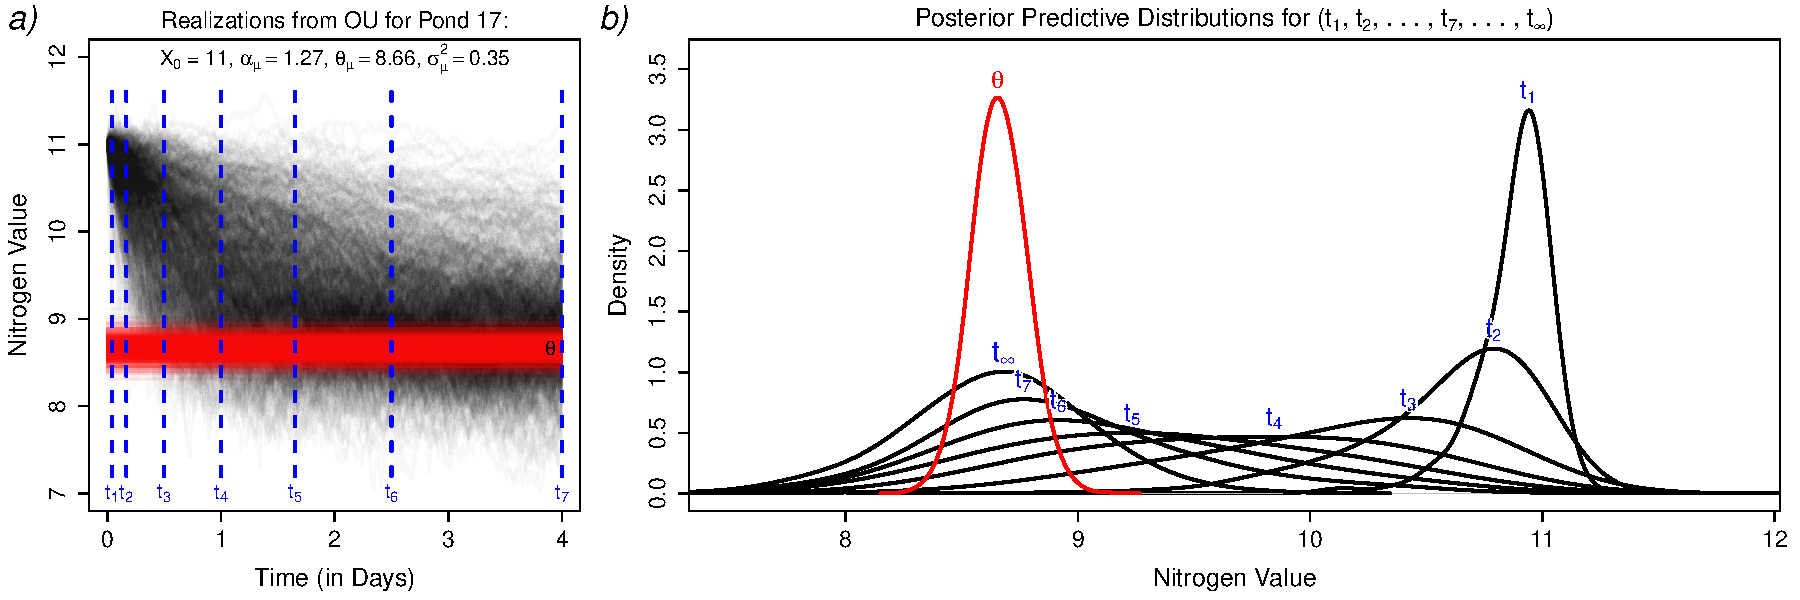
\includegraphics[width=160mm]{figures/OU_Ponds.pdf}
\caption[Posterior Predictive Distribution of a Hierarchical OU Model]{In a), realizations from an OU process over 4 days for Pond 17, averaging over posterior uncertainty. Mean values for all univariate OU model parameters are labeled, with samples from the posterior distribution for $\theta$ marked in red. The joint posterior distribution can be sampled and simulated from to generate posterior predictive distributions for arbitrary timepoints, marked with blue dashed lines. In b), kernel density plots of these posterior predictive distributions are provided, with corresponding timepoints labeled. A final timepoint, t$_\infty$, gives the limiting distribution for the process. The model used here was a hierarchical model, and could be analogized to a star phylogeny of manure ponds whose optima evolve on the tree according to a Brownian motion process, with returning force ($\alpha_i$) and rate ($\sigma^2_i$) parameters for each pond$_i$ estimated according to exponential hyperdistributions for each. \label{overflow}
\label{fig:OUPonds}}
\end{figure*} 

\subsection{Morphological Clock Models}
 
Another common modification made to the Brownian motion process in phylogenetic comparative contexts involves an allowance for the rate parameter to vary through time \citep{blombergTestingPhylogeneticSignal2003, harmonEarlyBurstsBody2010}. Specifically, one may set the Brownian motion rate parameter at time t ($\sigma^2_t$) equal to a product of the initial rate ($\sigma^2_0$) and the base of the natural logarithm (e) raised to the power of the product of some constant (r) and time (i.e. $\sigma^2_t$= $\sigma^2_0 e^{rt}$). If r is negative, rates will start off small and increase through time, leading to an Accelerating (AC) or Late Burst (LB) model of trait evolution. Meanwhile, if r is positive, rates will start off large and decrease through time, leading to a Declining (DC) or Early Burst (EB) model of trait evolution. If r is 0, the ACDC / Burst model collapses back into standard Brownian motion, as $e^{0t} = 1$ and $\sigma^2_t$ = $\sigma^2_0$. The inclusion of this extra layer, then, allows you to fit models that capture hypotheses pertaining to rapid diversification of form following a lengthy stasis, or vice versa. 

In practice, phylogenetic likelihood calculation under these relaxed clock models works by rescaling the branch lengths of a phylogeny according to the integral of the rate function along each branch. This consideration reveals that all these named variations on Brownian motion should not \textit{properly} be thought of as different character evolutionary models at all, but rather different \textit{clock} models, relaxations on the assumption of a strict morphological clock dictating proportionality between morphological evolution and either time or molecular evolution. So too should be considered other transformations of phylogenetic branch lengths, such as Pagel's $\lambda$, $\kappa$, and $\delta$ \citep{pagelMaximumLikelihoodApproach1999, pagelInferringHistoricalPatterns1999}, which are often interpreted to respectively measure ``phylogenetic signal'' (i.e., as an informal test of the strict morphological clock), association between diversification rate and morphological change, and more gradually slowing or speeding rates of evolution. For our purposes here, we typically place no strong constraints on variation in the rate of the morphological clock throughout a tree, preferring instead to set weakly informative, regularizing priors on branch lengths. As most of the analyses that follow lack an independent or jointly performed estimate of phylogeny on which morphological rate variation could be meaningfully considered, we instead infer trees whose branch lengths are in units of the square root of expected morphological change (specifically, the variance, $\sigma^2$ of a particle under Brownian motion scales linearly with branch length, and its expected absolute deviation can be found by evaluating twice the integral of the normal probability density function across (0, $\infty$), which equals $\sigma \sqrt{2 / pi}$). 

As in the preceding section, work done in association with but outside the strict scope of this dissertation explored our ability to retrieve parameters of relaxed morphological clocks --- for example, centering an evolutionary burst not at the root of the tree, but some distance into its branches. Here, we examined the role mass extinction events (specifically the Cretaceous–Paleogene) played in the evolution of fish feeding morphology (Figure \ref{fig:middleBurst}). In addition, a short simulation study identified the effects of such a ``middle-burst'' on disparity through time \citep{harmonTempoModeEvolutionary2003} plots (Figure \ref{fig:disparityThroughTime}), a heuristic and difficult-to-interpret attempt to capture phylogenetic rate variation.
 
\begin{figure*}[h]
\centering
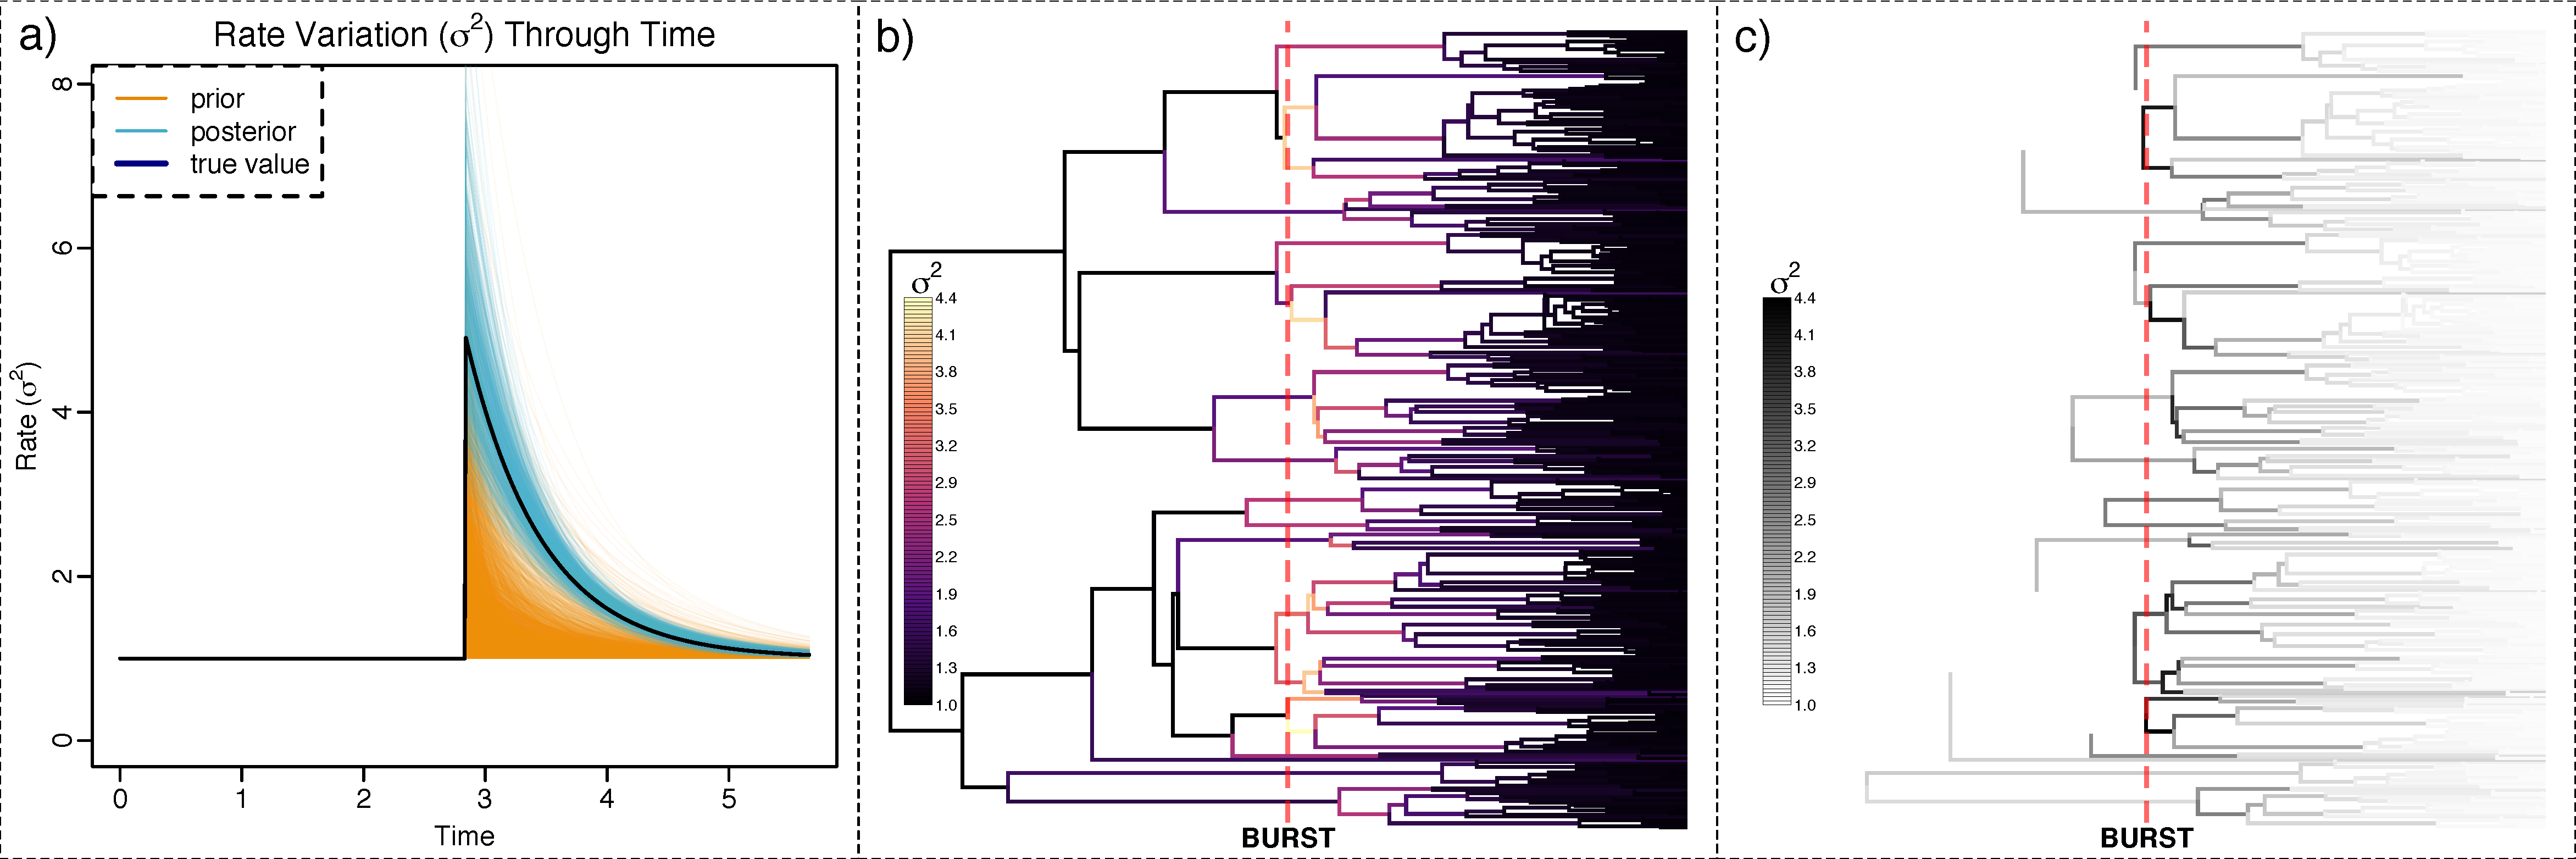
\includegraphics[width=160mm]{figures/middle_burst.pdf}
\caption[Posterior Distribution of a Middle Burst Brownian Motion Model]{The result of a single simulation experiment attempting to infer the magnitude and decay constant of an evolutionary burst of known location given a known tree with 450 tips and univariate character data. In a), samples from both the prior and posterior are plotted and labeled, with the true value of the burst shown in dark blue. In b-c), branch-rates are plotted on the phylogeny used with color-coding and on a white-black gradient, respectively. 
\label{fig:middleBurst}
\label{overflow}}
\end{figure*} 

\begin{figure*}[h]
\centering
\includegraphics[width=160mm]{figures/expected_disparity_through_time.pdf}
\caption[Variation in Expected Disparity Through Time Under Varying Middle Bursts]{An exploration of the expected trend of a disparity through time plot for a tree with 300 taxa. In a), the relaxed morphological clock model is shown, featuring a change in evolutionary rate at the temporal middle of the tree, followed by an exponential decay to normalcy. The magnitude and direction of the change is given by $\Delta$, and expected trends for different values of $\Delta$ are shown in panel b). 
\label{overflow}
\label{fig:disparityThroughTime}}
\end{figure*} 
  
%Figure 3. 50 independent replicates for both an Early Burst and a Late Burst process over 100 time steps with a starting state of zero. In the Early Burst model, r was -0.05 and the starting rate was 100; in the Late Burst model, r was 0.05 and the starting rate was 1. 

\clearpage

\section{Benefits of Working in a Bayesian Inferential Framework}

Model-based inference is preferred in part because of the flexibility it affords --- should something in the set of considered models dissatisfy, it can be straightforward to engineer a better model, one more able to capture the suspected underlying biology responsible for generating empirical data. But having committed ourselves to the likelihood principle, we encounter a further dilemma: should the model be fitted in a (penalized) Maximum Likelihood framework, searching for the most plausible set of model parameters? Or should we instead try to reach a compromise between the information contained within our data, as perceived by our likelihood function --- and our prior beliefs about the probabilities of different model parameters? As the title of this work suggests, we generally opt for the latter strategy, carrying out most inference in a Bayesian framework. This is despite objections raised by both those in favor of Bayesian approaches \citep{gelmanHolesBayesianStatistics2020} and those out of favor \citep{gelmanObjectionsBayesianStatistics2008}. Our motivations in these regards are many and are described below:

\paragraph{Interpretability}

Though Bayes' theorem is, at heart, a trivial implication of introductory probability theory, it provides an elegant, powerful, and necessary vehicle by which to obtain probabilistic estimates of model parameters. Most scientists' statistical intuitions naturally hew close to Bayesian interpretations of probability \citep{kaplanNullRitualWhat2004}, and accommodating inferential uncertainty and evaluating the degree of support in the data for competing hypotheses is much simpler with a probability than with devices such as the non-parametric bootstrap \citep{efronBootstrapMethodsAnother1979, felsensteinConfidenceLimitsPhylogenies1985}. When prompted, most practitioners default less to thinking in terms of sampling distributions of estimators and more to interpreting p-values or bootstrap support estimates as probabilities of alternative hypotheses \citep{greenlandStatisticalTestsValues2016}. Performing the non-parametric bootstrap in a multivariate framework would also require additional data transformation before resampling, as any data resampled with replacement would necessarily be perfectly correlated with itself, incapable of contributing additional phylogenetic information.

\paragraph{Prior Information}

Though often viewed as a detriment, Bayesian inferences allows for the incorporation of prior information into our analyses, forcing us to explicitly encode our beliefs about the model in greater detail than just those assumptions implicit to our choice of likelihood function (equivalent to point-mass priors on parameters of some higher nested model). We can specify prior distributions on model parameters as informatively or uninformatively as we feel justified, and further evaluate the extent to which results are sensitive to our choice of priors by running the model under different combinations of prior distributions and contrasting the resultant posterior distributions. When analyzing data, we rarely think that all possible supported parameter values are equally plausible: trees are unlikely to be a trillion units long, and evolutionary rates probably will not vary by dozens of orders of magnitude. Why \textit{not} incorporate this prior information into our analysis in the most principled possible way?

\paragraph{Regularization}

Beyond, encoding our prior beliefs about the data-generating process, priors also serve an important role in preventing undue excitation of the likelihood function in regions of parameter-space that fit especially well to the data, despite not being intrinsically plausible. In so doing, priors help us to tread the line between overfitting and underfitting, balancing error resulting from the model learning from noise in the data with error from the model being insufficiently flexible. In phylogenetics, priors can help us tease apart otherwise non-identifiable parameters whose combination forms a ridge in the likelihood surface, such as clock rates and time during divergence time estimation. They also help us to avoid capture of the model by singularities in that surface, such as when estimating both the value and parameters of a normally distributed random variable (for example, if jointly estimating tip states and the branch lengths separating them under Brownian motion). Hierarchical model structure also lets the model itself learn how skeptical it should be about extreme parameter values, adaptively regularizing priors only to the extent justified by the data \citep{gelmanWhyWeUsually2012}. This strategy finds extensive application in other work, including non-phylogenetic side projects performed in association with this dissertation, but is also used in the catarrhine landmark and discrete dental analyses to flexibly tune the amount of rate variation between traits and branches permissible in those applications. In this manner, we allow the model to partially pool information between parameters, lending aid from highly concentrated regions of the joint posterior to those more diffuse. Though less of a concern in phylogenetic applications, adaptive regularization also helps us to avoid multiple comparisons problems \citep{gelmanWhyWeUsually2012}, such as when we do inference over dozens of rates and examine the ones assessed to be more or less confidently determined.

\paragraph{Stability}

In cases where the likelihood surface is multimodal, Bayesian inference may more easily traverse the distance between peaks than a stochastic optimization algorithm, arriving at more robust estimates of model parameters than mere search for phylogenetic optima. When performing empirically parameterized simulation studies, sampling from the posterior distribution of an analysis of real-world data also helps to better represent the problematic nature of real-world data than the idealization of trees samples from parametric distributions or the simulation invariance of using a single phylogenetic Maximum Likelihood Estimate (MLE). As we use numerical algorithms to approximate joint posterior distributions, we also find ourselves endowed with the tools to assess their reliability. A purported MLE might actually represent a local maximum, with little diagnostic recourse but to compare the output of multiple independent runs, but MCMC output can be screened with many devices to ensure healthy chain mixing and convergence over and on the target distribution.

\section{Prospectus}

A table of contents appears at the start of this work, but it is also fitting to describe what is to come in prose. The ultimate goal of this work was to adapt the threshold model of quantitative genetics to the purpose of inferring phylogeny, and in particular the topologies of trees scaffolding the evolution of high-dimensional ordinal character data (Chapter \ref{chpt:Chapter4}). The primary empirical application of this work was an alignment of ordinal dental traits codified in the Arizona State University Dental Anthropology System \citep{turnerScoringProducesKey1991} and collected by Dr. Shara Bailey. Before that could be done, we first needed to develop and implement a multivariate Brownian model of character evolution, as well as explore its statistical properties in simulation (Chapter \ref{chpt:Chapter2}). Here, we applied the method to a publicly available, open-source dataset of craniofacial linear measurements collected by William W. Howells \citep{howellsCranialVariationMan1973, howellsSkullShapesMap1989, howellsWhoWhoSkulls1995}. In between these, we also compare the performance of our multivariate Brownian motion model to a menagerie of methods commonly used to infer phylogeny using morphology on a cranial landmark dataset collected on 13 different species of catarrhine primate by Katerina Harvati (\citeyear{harvatiNeanderthalTaxonomyReconsidered2004}) and colleagues (Chapter \ref{chpt:Chapter3}). Trees from these analyses could be compared to a well-resolved reference tree obtained from a published analysis of molecular data \citep{arnold10kTreesWebsiteNew2010}, that the yardstick of method performance not be exclusively fictitious, in the sense of agreement with some simulated ground-truth, but also relate in some way to biological reality.

Mathematical details are scattered throughout these chapters, though hopefully not in too overwhelming or tiresome a frequency. Three supplemental appendices (\ref{app:App1}, \ref{app:App2}, and \ref{app:App3}) are also included in the closing sections detailing further details that the main text could not stand to bear. A concluding section (Chapter \ref{chpt:Chapter5}) summarizes key takeaways and provides a roadmap for follow-up research.

%\AddToShipoutPictureFG*{\put(435,-15){\includegraphics[width=60mm,scale=1]{figures/bayesianBodybuilder.png}}}

%Partial pooling of information between groups / classes – avoid multiple comparisons problems!
%Allows for more intuitive model averaging / comparison?
%MCMC potentially more stable / robust if likelihood surface multimodal vs. optimization algorithms
%NHST is silly
%
%Once we’ve implemented an algorithm to calculate the likelihood of a fully specified phylogenetic model (i.e. topology, branch lengths, and evolutionary model parameters), we can use it to conduct inference according to Bayes Theorem, which states that P(model | data) = P(data | model) * P(model) / P(data), or alternatively, Posterior = Likelihood * Prior / Average Likelihood, with priors assumed beforehand (though we can also “infer” priors from the data by using hyperpriors, or use for priors the posteriors of some earlier analysis). Calculating the average (also called the marginal, because it marginalizes across all possible combinations of parameters) likelihood is tricky, but thankfully, it’s just a constant, there to standardize the posterior and make sure the whole distribution integrates to 1. Markov chain Monte Carlo (MCMC) can sample from the joint posterior in proportion to its probability at any particular combination of parameters, eliminating the need to calculate the average likelihood (by accepting proposed changes in proportion to the ratio of posterior probabilities of the proposed and current states of the chain, so the average likelihoods in the numerator and denominator cancel out). Alternative methods to estimate the joint posterior exist, such as grid and quadratic approximation (McElreath 2015), but they won’t work here: the latter isn’t compatible with the discrete “tree topology” parameter – what’s a normal distribution of trees, anyway? – and the joint posterior of continuous parameters is unlikely to be multivariate normal. The former, meanwhile, scales poorly with larger numbers of parameters, so even branch lengths alone, if allowed to vary freely, would ensure that computation takes a very, very long time.  
%
%There are a number of MCMC sampling algorithms, one of which will ultimately have to be chosen and implemented, that differ largely in how they make proposals to move to new parts of parameter space. Where the Metropolis algorithm can only make symmetric proposals, the Metropolis-Hastings algorithm allows for asymmetric proposals (useful for parameters with constraints – e.g. branch lengths can never be less than 0), and Gibbs and Hamiltonian samplers adjust their proposal mechanisms intelligently to draw from the joint posterior more efficiently. Proposal mechanisms will have to be chosen and tuned beforehand, too – how we move through parameter space can greatly affect how well we conduct sampling. After we sample, MCMC health is a pressing concern, and diagnosing chain performance issues can be done in a number of ways: by looking at the number of effective, independent samples from the posterior and autocorrelation time between samples, visually inspecting time-series trace plots of multiple chains for single parameters, as well as marginal posterior densities from independent chains, using various diagnostics, like the Gelman-Rubin convergence diagnostic (Gelman and Rubin 1992), the Geweke diagnostic (Geweke 1991), and the Heidelberg-Welch diagnostic (Heidelberg and Welch 1983), ensuring acceptance rates are intermediate, and so on. Mike May’s releasing a program called BONSAI (Bayesian Output Needs Semi-Automated Inspection) sometime soon that automates MCMC diagnosis and will undoubtedly be useful in examining chain health. 
% 
%Bayes is all about accommodating uncertainty, which is great, since there’ll be a lot of uncertainty to accommodate here. For one, it’s unclear how much phylogenetically relevant information is in morphology in the first place, but millions of “independently” evolving loci it is certainly not (and measures of phylogenetic signal can be ambiguous even when data is explicitly simulated on a phylogeny, Münkemüller et al. 2012; for example, Pagel's $\lambda$, which rescales internal and external branches on a tree, is estimated especially poorly when trees are small, Boettiger et al. 2012). Where Maximum Likelihood might confidently tell us that, yes, this is the ML set of parameters (and, with the non-parametric bootstrap, they are stable with respect to resampling of the data), it wouldn’t quite represent uncertainty in inference in an intuitive, immediately grokkable way (e.g. bootstrap values can’t be interpreted as probabilities, as a lot of your data might definitively, but weakly support some set of parameters over another. Resampling such data would get very high bootstrap values, but you still shouldn’t have much confidence in the results. Bootstrapping is computationally costly, too – having however many bootstrap replicates means you have to redo your entire analysis that many times! Similar reservations apply to the jackknife). 
%
%Additionally, measurement error, sampling intensity, and missing data are important issues to consider. Recall, for example, that we’re modeling changes in the mean values of continuous traits in a given lineage. Sample sizes in our tips vary, so modeling observations not as single vectors of means but as distributions (say, a multivariate normal, with standard deviations equal to the estimated standard error of the mean, SEmean = SDsample / (sample size)1/2) is easy enough to do in a Bayesian framework (McElreath 2015). Same goes for counts of discrete traits – we’d be a lot more certain that the mean liability is near the threshold when we observe that 27/54 individuals express a trait than when we observe that 3/6 individuals have it. Inter- and intra-observer error are additional concerns with discrete dental traits, as the measurement process is a bit more subjective than, say, reading a number off some calipers, but that source of uncertainty can also be incorporated into our analysis.   
%
%Wholly and partially missing data are also a concern (Guillerme and Cooper 2016, Pattinson et al. 2014), at least with respect to discrete dental traits (Howells’ data set is more complete, perhaps because we rarely use our skulls grind down sharp objects, lose bits of them piece by piece, or expose them to cariogenic bacteria). Imputation can help us there by modeling and inferring missing values as a distribution conditioned on data that is present. Some questions will need to be answered and decisions made, however, like whether the data missing completely at random (MCAR). It might be that certain values of discrete traits make them more prone to absence through pathology – a large groove might give bacteria a nice environment in which to grow, making tooth loss more common in those individuals with large grooves. In any case, we’d need to make the MCAR assumption to exclude cases with missing data (McElreath 2015), and imputation lets us not throw away perfectly good information alongside that which we lack.  
%
%Data can be “partially missing” as well, in the sense that wear can obscure the expression of certain traits, leading to bias that exaggerates or diminishes the frequency with which they are present. For example, dental wear can wipe out or reduce the size of small cusps, causing researchers to record them as absent. Alternatively, it can make traits like the middle trigonid crest look continuous when they’re actually interrupted (Shara Bailey, personal communication). If researchers score traits as present only when they are clearly present, and wear makes observed expression ambiguous, frequencies can be biased downward due to “partially missing” data (Burnett et al. 2013). When recording dental trait expression, it’s important also to record the extent to which teeth are worn, perhaps by noting the size and frequency of wear facets and dentine patches (e.g. Molnar 1971). This information can then be incorporated into our analysis by widening the distribution of modeled observations or skewing it if the direction of bias can be identified. 
% 
%It may also be important to account for the possibility of sampling (or acquisition) bias when using the ASUDAS traits. The ASUDAS was developed specifically to describe dental variation between populations, and this emphasis on variant characters could result in inferred branches being too long, which might in turn introduce bias to our inference of tree topology (indeed, one could say that nonsynapomorphic traits like symplesiomorphies are phylogenetically informative!). This is a concern with inference under the Mk model for which corrected Mkv and Mk-pars models have been developed (Lewis 2001).  Perhaps we will need something similar here, too. 
% 
%Additionally, Bayesian models are generative, which is to say that we can use them to simulate fake data. We can then apply our inferential methods to this fake data to see if we can correctly estimate the parameters under which we initially performed the simulations under. In particular, we might be interested if we can infer the tree topology parameter correctly, and if we can’t recover it perfectly, how well we might still be able to do. A number of metrics have been developed to compare tree topologies, such as the Robinson-Foulds distance (Robinson and Foulds 1981), for which a generalized form also exists (Böcker et al. 2013) and the subtree-prune-and-regraft distance (dSPR; SPR refers to an intermediate mechanism of rearranging trees and moving through tree space; Hickey et al. 2008). These can be applied across simulations to see, on average, how poorly or how well our methods can infer the true data-generating $\Psi$, as well as to assess statistical consistency as we simulate more and more observations. 
%
%Simulation is also helpful when conducting power analysis. If it turns out that we can reliably infer the true trees, but we need to have a certain number of tips or individuals or traits to do so, I can go out and collect more data for unrepresented or poorly represented populations (e.g., in Dr. Bailey’s ASUDAS dataset, Native American, Asian, Eastern European, and Southern European populations don’t feature as strongly. Specimens from these geographic regions are contained at the Field Museum in Chicago, IL, at the Arizona State Museum in Tucson, AZ, and at the Center for Archaeology and Society at Arizona State University in Tempe, AZ, as well as in collections throughout Eurasia and Australasia, such as the Biological Anthropology Collections at the University of Tokyo, the Australian Museum, and the Parisian Musee del’Homme). But visiting museums to collect data on these populations absent an explicit power analysis risks my either oversampling a particular population (when I could be sampling a different population) or undersampling that population (and so not being able to say anything meaningful about it). Therefore, data collection should be temporarily postponed until I can better leverage the theoretical framework I’ll be developing in the course of my research and say with confidence how much and what sort of data I need to collect. 
% 
%Finally, when the method and the data are both squared away, I can attempt to infer phylogeny using only morphological traits, and compare the results to trees obtained from nucleotide sequence alignments representing the same populations. This is especially important, as phylogenetic analyses based on craniodental data using other methods have historically failed to infer the correct trees (Collard and Wood 2000). Using sequence data obtained from the Human Genome Diversity Project (or off GenBank), which has genotyped 660,918 markers in 1043 individuals from 52 globally distributed populations (Cavalli-Sforza 2005), “true” trees can be inferred with cutting-edge methods in RevBayes and compared to those obtained from morphological data. Analyses can also be conducted to assess the performance of different implementations of the Mk model (for both continuous and discrete traits – we can always bin the former), Maximum Parsimony, and distance-matrix methods. Even if the methods I develop are bad, perhaps they can be less bad than all available alternatives, and therefore still be of some use to those hoping to infer phylogeny using morphology alone (e.g. Irish et al. 2013, Dembo et al. 2015). 


\clearpage



\include{chapter1_mvBM}
\chapter[Primate Phylogenetics with Landmark Data]{Primate Phylogenetics with Landmark Data: \\Exploring Model-Based and Heuristic Approaches}

\label{chpt:Chapter3}

\chapterauthor{Nikolai G. Vetr, Timothy D. Weaver}

\clearpage

\section{Abstract}

Paleontologists and paleoanthropologists have long sought to better understand evolutionary relationships linking fossil and extant taxa. While modern genetic and genomic methods offer ample opportunity for phylogenetic inference, age and degradation quickly limit adequate retrieval of ancient DNA from fossil specimens. New approaches extending phylogenetic models common in the comparative methods literature could conceivably improve inference of fossil phylogeny over more commonly used heuristic methods developed prior to recent decades' advances in computation and theory. Here, we explore the application of a stochastic multivariate Brownian diffusion model to a set of landmark data collected across a range of catarrhine primate species. We contrast results from this fitted model to those obtained from Bayesian analysis of matched molecular data, as well as to results from more conventional, heuristic inference procedures, such as distance-based methods and Maximum Parsimony. A short simulation study is also performed to explore the behavior of the multivariate Brownian method under empirically parameterized conditions. With the advent of increasingly sophisticated continuous character data capture technologies, improved understanding of how different methods perform will help to inform researchers' phylogenetic analyses and better infer the evolutionary relationships connecting both fossil and extant taxa. [Primate Evolution; Bayesian Inference; Multivariate Brownian Motion]

\clearpage

\section{Introduction}

Phylogenies are inferred representations of the branching process of speciation, the splitting of ancestral populations into reproductively isolated daughter lineages. Evolution makes little sense except in their light. But far from merely depicting genealogical relationships among taxa of interest, their inference is essential to the investigation of many evolutionary questions. Perhaps most importantly, they serve as a scaffold for the analysis of character evolution \citep{felsensteinPhylogeniesComparativeMethod1985}, as shared ancestry confounds relationships between traits observed in taxa evolving along the branches of phylogenetic trees. They also provide a framework for divergence time estimation \citep{glazkoEstimationDivergenceTimes2003, heathBayesianInferenceSpecies2014}, ancestral trait reconstruction \citep{schluterLikelihoodAncestorStates1997, joyAncestralReconstruction2016}, species delimitation and taxonomic classification \citep{rannalaArtScienceSpecies2015}, historical biogeography \citep{donoghueIntegrativeHistoricalBiogeography2003, ronquistPhylogeneticMethodsBiogeography2011}, analysis of lineage diversification \citep{neeReconstructedEvolutionaryProcess1994, morlonPhylogeneticApproachesStudying2014}, and much more. They can help to generate, constrain, and discriminate between paleontological hypotheses, guiding our interpretation of the fossil record. Whether some species is ancestor, sister, or descendant to some other species; whether the same character evolved many times, convergently, or just once; whether suites of characters coevolved simultaneously or appeared piecewise; these and other questions can be explicitly explored within a phylogenetic framework. 

Likely owing to our own taxonomic affinities and the wide availability of both morphological and molecular data, primates -- especially the catarrhine primates --  serve as a common target for the application of new phylogenetic methods or the exploration of existing methods \citep[e.g.][]{reisUsingPhylogenomicData2018} and as examples in tutorials demonstrating the use of phylogenetic software (e.g. in Beast or RevBayes; \citealt{bouckaertBEASTAdvancedSoftware2019}; \citealt{hohnaRevBayesBayesianPhylogenetic2016a}). Though most recent analyses of primate phylogeny focus on molecular data \citep[e.g.][]{perelmanMolecularPhylogenyLiving2011, springerMacroevolutionaryDynamicsHistorical2012}, historical attempts at inference made use primarily of morphological characters, despite their arguable unreliability at retrieving trees compatible with molecular results \citep[e.g.][]{collardHowReliableAre2000, gibbsSofttissueCharactersHigher2000, varon-gonzalezEstimatingPhylogeniesShape2020}. When inferring phylogeny among fossil taxa, paleontologists are often limited to the use of morphological characters, as degradation quickly limits the ages of fossils from which ancient DNA can be successfully extracted, sequenced, and assembled \citep{collinsSurvivalOrganicMatter2002, allentoftHalflifeDNABone2012, pickrellNewHistoryGeography2014}. Among hominins, for example, attempts to infer phylogeny have made use of a panoply of algorithms -- described briefly below -- to transform some alignment of morphological character data into a point estimate or set of phylogenetic trees. There exists a long history of these attempts, stretching many decades into the past \citep[e.g.][]{chamberlainEarlyHominidPhylogeny1987, stringerNumericalCladisticAnalysis1987, skeltonEvolutionaryRelationshipsEarly1992, straitReappraisalEarlyHominid1997}, but also in recent years \citep[e.g.][]{irishDentalMorphologyPhylogenetic2013, demboBayesianAnalysisMorphological2015, demboEvolutionaryRelationshipsAge2016, argueAffinitiesHomoFloresiensis2017}. To further inform practice in these contexts, it is useful to explore the performance of newer, model-based methods for inferring phylogeny using morphological characters, contrasting their output with results from more conventional approaches, such as Maximum Parsimony or distance-based methods. A natural system for such a comparison can be found, of course, in the catarrhine primates.

The most popular inference model for phylogenetically structured morphological data is Lewis’ (\citeyear{lewisLikelihoodApproachEstimating2001}) Mk-model, which can be fit in both Bayesian and Maximum Likelihood frameworks. For four-state characters, it is identical to the Jukes-Cantor (\citeyear{jukesEvolutionProteinMolecules1969}) model of nucleotide substitution (as the canonical state-space of DNA is 4), and otherwise generalizes the Jukes-Cantor model to arbitrary numbers of states. This model is well explored in phylogenetic contexts, both in the nucleotide substitution case and for discrete morphological characters \citep[e.g.][]{wrightModelingCharacterChange2016}. Fitting this model under maximum likelihood produces a point estimate of tree topology, branch lengths, and evolutionary model parameters that corresponds to the parameter values under which the observed data are most plausible (the Maximum Likelihood Estimate, or MLE). Conversely, the Bayesian target of inference is the entire joint posterior distribution of phylogenetic model parameters, often approximated numerically with Markov chain Monte Carlo (MCMC).

Other phylogenetic inferential methods commonly applied to morphological datasets include tree-search under the Maximum Parsimony (MP) criterion and some cost matrix, as well as clustering algorithms (e.g. neighbor joining or UPGMA) that accept as input some distance matrix and produce as output a tree with particular properties. Both typically also produce point estimates, though one can envision procedures (e.g. the non-parametric bootstrap; \citealt{efronBootstrapMethodsAnother1979}; \citealt{felsensteinConfidenceLimitsPhylogenies1985}) that incorporate sampling or measurement uncertainty, as one might also do with Maximum Likelihood inference. For MP methods, often there can be obtained a set of distinct most parsimonious or nearly-most parsimonious trees, but how one probabilistically interprets the frequency of clade membership in this set is unclear. Parsimony can also mislead under certain conditions even at the limit of infinite data, such as when evolutionary rates are high or heterogenous \citep{wrightBayesianAnalysisUsing2014, wrightModelingCharacterChange2016, oreillyProbabilisticMethodsSurpass2018}, and typically requires the use of independent, discrete characters. Distance methods can calculate distances that incorporate evolutionary models of character change, but also struggle to accommodate inferential uncertainty in a principled manner, especially in a multivariate framework where resampling characters cannot, by construction, supply any further phylogenetically meaningful information. 

Frequently, morphological variation between groups is not discrete, but continuous. While distances can easily be computed between sets of continuous characters, inference under the Mk-model \citep{lewisLikelihoodApproachEstimating2001} and most parsimony-based methods \citep{goloboffContinuousCharactersAnalyzed2006} often require that we discretize any continuous observations. Continuous forms of MP algorithms do exist, such as Squared-Change Parsimony \citep{maddisonSquaredchangeParsimonyReconstructions1991, rohlfGeometricMorphometricsPhylogeny2002}, Linear Parsimony \citep{klugeQuantitativePhyleticsEvolution1969}, Manhattan-Metric Parsimony \citep{swoffordInferringEvolutionaryTrees1987}, and others \citep[see][]{rogersComparisonSuitabilityRogers1991}, but these are almost always applied to quantitative characters in the service of ancestral state reconstruction and not the inference of tree structure itself, and so will not be directly considered here. Discretization can be done in a variety of ways \citep{garcia-cruzCodingQuantitativeCharacter2006, thorpeCodingMorphometricCharacters1984} in part subject to researcher preference, with some methods retaining more phylogenetic information than others \citep{brazeauProblematicCharacterCoding2011, worthingtonSelectionCharacterCoding2017}. Even discrete characters collected at the outset may just be discretizing some fundamentally quantitative feature \citep{wiensCharacterAnalysisMorphological2001}, relying on a researcher's present observations and prior experiences instead of an explicit algorithm run on the character alignment in its entirety. Recent decades have also witnessed the rise of new techniques for the collection of continuous morphological data, such as surface and CT scanning \citep{mitteroeckerAdvancesGeometricMorphometrics2009, adamsFieldComesAge2013, reinGeometricMorphometricsVirtual2014}. As such, we may desire to better understand statistical methods for inferring phylogeny that can make direct use of continuous characters without needing to discretize them. 

Inference under a multivariate Brownian motion model of character evolution may satisfy this desire. Multivariate Brownian motion (mvBM) is a straightforward extension of univariate Brownian motion \citep{felsensteinMaximumlikelihoodEstimationEvolutionary1973}, modifying only that displacements to character states be drawn from multivariate normal distributions, rather than univariate normal distributions. This allows for the representation of phenomena such as pleiotropy, correlated selection, linkage, and integration, which may structure the evolution of quantitative traits. Here, we investigate how well an mvBM model fit in a Bayesian statistical framework is able to retrieve catarrhine phylogeny using 15 3-Dimensional craniofacial landmarks sampled across a collection of 13 catarrhine primate species \citep{harvatiNeanderthalTaxonomyReconsidered2004}. We compare this inference to those obtained from other parametric models of character evolution, both distance-based and Maximum Parsimony methods, as well as to relationships in this group inferred from molecular data \citep{arnold10kTreesWebsiteNew2010}. We then perform a short, empirically realistic simulation study under mvBM to explore the performance of the method in its ability to retrieve true, data-generating trees and clades when the inference model is well specified. 

\clearpage

\section{Materials and Methods}

Empirical data used in this analysis were drawn from the (\citeyear{harvatiNeanderthalTaxonomyReconsidered2004}) work of Harvati and colleagues and consisted of 15 3-dimensional craniofacial landmarks sampled on 13 species of catarrhine primate. Samples were also partitioned at the subspecific level, with 7 populations of \textit{Homo sapiens}, 6 subspecies of \textit{Papio hamadryas}, 3 subspecies of \textit{Pan troglodytes}, and 2 subspecies of \textit{Gorilla gorilla} present in the dataset, for 27 total tips at maximum taxonomic resolution. Given the extent of hybridization known to occur between subspecies and populations --- for example, in \textit{Papio hamadryas} \citep{rogersComparativeGenomicsComplex2019} --- we lumped together all divisions in the data below the species level, that their phylogeny might be better represented by a non-reticulate, strictly bifurcating tree. Sample sizes for extant species ranged from 17 for \textit{Macaca hecki} to 400 for \textit{Papio hamadryas}; the only extinct species in the analysis, \textit{Homo neanderthalensis}, was also present in the fewest number, with 5 sampled individuals. Information regarding the composition of this dataset can be found in Table \ref{tab:landmarkDataComposition}, with more information on the precise sample composition and locations of specific landmarks able to be found in the aforementioned paper \citep{harvatiNeanderthalTaxonomyReconsidered2004}. These data also contained information on each individual's estimated sex, and to avoid the confounding effects of sexual dimorphism we treated sex-specific observations as representing separate, independently evolving partitions, pooling information across partitions with respect to topology but otherwise independently estimating phylogenetic model parameters. In other words, we specified an evolutionary model where male and female morphologies were able to evolve independently from one another, constrained only in that the branching order of speciation events had to be identical for both. Given the non-independent nature of within-species male and female morphology, this may induce some degree of pseudo-data-duplicatory effect, but additional pooling of model parameters was judged inappropriate given further transformations described below.

This dataset has several features that make it desirable for the analyses performed here. The species included are not only highly studied but also of intrinsic interest, with well ascertained molecular phylogenies available for comparison. Additionally, the landmark nature of the data makes exploring the statistical performance of modern multivariate phylogenetic methods especially enticing, given the projected proliferation of these datasets as morphologists continue to develop semiautomated landmark capture techniques. Past attempts to infer phylogeny using craniofacial morphology have met mixed success \citep[e.g.][]{collardHowReliableAre2000}, so assessing the performance of different methods with respect to both empirical and simulated data may help to inform researchers' decisions when analyzing landmark data from other systems. 

Before the data could be analyzed, several pre-processing steps were required. First, we performed Procrustes transformation \citep{gowerGeneralizedProcrustesAnalysis1975, drydenStatisticalShapeAnalysis2016} on all data irrespective of sex simultaneously, scaling the set of each individual's landmarks to unit centroid size and iteratively rotating and translating until the Procrustes distances across all individuals' landmarks converged to some minimum value \citep{booksteinLandmarkMethodsForms1997}. This was done using the \texttt{gpagen()} function in the \textit{geomorph} package \citep{adamsGeometricMorphometricAnalyses2019} in \textit{R} \citep{rcoreteamLanguageEnvironmentStatistical2013}. Following Mitteroecker and colleagues (\citeyear{mitteroeckerComparisonCranialOntogenetic2004}) and to allow size and not just shape to inform subsequent analyses, log-centroid size was reintroduced as a single additional variable, bringing the total number of traits used to 46 (3 x 15 shape coordinates + size). 

However, the evolution of these 46 traits is not independent, and so we might attempt to correct for this nonindependence before attempting any phylogenetic analysis. To do this, we compute the sex-specific pooled within-group covariance matrix of our transformed landmark data, $P$. Under Cheverud's conjecture \citep{cheverudDevelopmentalIntegrationEvolution1996}, this should be proportional to the additive genetic covariance matrix, $G$, which describes the variances and covariances of morphological evolution at mutation-drift equilibrium \citep{weaverNeutralTheoryEvolution2018a}. However, as Procrustes transformation removes 7 degrees of freedom (1 for translation and rotation in each of the three dimensions, 1 for scaling), the resulting $P$ matrix is rendered non-positive-semidefinite --- with seven negative eigenvalues trailing --- and therefore uninvertible, which makes it unsuitable for use in, for example, an informative prior for the multivariate Brownian motion rate matrix. To circumvent this limitation, we decompose P into its eigensystem, with columns of the eigenvector matrix ordered according to monotonically decreasing eigenvalues. We then project the Procrustes transformed landmarks onto those eigenvectors corresponding only to the positive eigenvalues, and further divide them by the square root of each corresponding eigenvalue, effectively transforming the 46 original characters into 39 whose pooled within-group covariance matrix equals the identity matrix. As a further dimensionality reduction step, we examine the scree plot of our eigensystem and discard those later axes comprising the final 1\% of the total variance, restricting ourselves to the minimum set of axes corresponding to 99\% of the total within-group variance, and reducing the number of characters to be analyzed to 19 in the female partition and 20 in the male. Thus, subsequent analyses assume that evolution can only occur within a lower dimension subspace along these principal axes, which do not span the entire space of our 46 characters, but may nevertheless allow for it to realize most of the variation observed in the empirical data. We relax this assumption and allow for greater non-independence in the Brownian motion model, but otherwise treat these normalized scores as independent outcomes of the evolutionary data-generating process.

To incorporate information from both sexes into the heuristic analyses performed here, we were not able to specify separate data partitions with greater or lesser degrees of parameter pooling, as heuristic methods lack a formal description of the data-generating process. Instead, we treated scores on each of the axes as independent observations for each tip, concatenating them into a single morphological character alignment.

Finally, no female Neandertals were present in the morphological dataset. To allow for the joint analysis of both partitions in phylogenetic software, we required equality between the sets of tips in either partition. Preliminary male-specific analysis found that Neandertals and \textit{Homo sapiens} clustered together with high confidence regardless of method or model used, so to construct a fictitious female Neandertal we found the vector difference between the two species means of male genus \textit{Homo} and displaced the female \textit{Homo sapiens} mean by that difference. This was done after the joint Procrustes transformation but before projection of species means onto each respective $P$'s eigenvectors, with the fictitious female Neandertal then projected onto the female $P$'s eigenvectors and included in the female partition for analysis.

Some methods required additional pre-processing, the details of which can be found below. In total, we inferred catarrhine phylogeny using three heuristic methods: UPGMA, Neighbor-Joining, and Maximum Parsimony; as well as under four models in a Bayesian framework: univariate Brownian motion, multivariate Brownian motion, Lewis' Mk model, and an ordered Continuous Time Markov Chain (CTMC) model. Each is described in turn. 

\subsection{Distance-Based Methods}

Two clustering algorithms served our purposes here -- the Unweighted Pair Group Method with Arithmetic mean algorithm \citep{sokalStatisticalMethodEvaluating1958} and the Neighbor-Joining algorithm \citep{saitouNeighborjoiningMethodNew1987}. Both were implemented in R as the functions \texttt{upgma()} and \texttt{nj()} in the \textit{phangorn} \citep{schliepPhangornPhylogeneticAnalysis2011} and \textit{ape} \citep{paradisAPEAnalysesPhylogenetics2004} packages, respectively. These methods require that we provide them a distance matrix, which they then use to construct either a rooted ultrametric tree or an unrooted tree with identical patristic distances (with elements of the distance matrix equal the sums of branch lengths separating tips). To compute a distance matrix, we needed a measure of distance between pairs of taxa. For this, we used the Euclidean distances between our transformed traits, similar to using a squared Mahalanobis distance \citep{mahalanobisGeneralizedDistanceStatistics1936} with $P$ serving to standardize distances between tips, as under our transformation of the character data, $P$ became the identity matrix. 

\subsection{Data Discretization}

Both the maximum parsimony analyses and many popular parametric evolutionary models require that data be discrete, rather than continuous. A number of approaches were available here, and we explored two. For the first, we followed the divergence coding procedure favored by Collard and Wood (\citeyear{collardHowReliableAre2000}, \citeyear{collardHowReliableAre2001}) and described by Thorpe (\citeyear{thorpeCodingMorphometricCharacters1984}). This assigned each tip a discrete character in the range ($1, 2, ..., 2n_{tips} - 1)$) and may better accommodate differences in the spacing between tips along a continuous scale, with larger differences corresponding to greater required amounts of evolutionary change. Conversely, the second discretized our continuous character ranges into intervals according to Jenks Natural Breaks Optimization Method \citep{jenksDataModelConcept1967}, implemented via the \texttt{classIntervals()} function in the \textit{classInt} package \citep{bivandPackageClassInt2020} in \textit{R}. Jenks' algorithm identifies a pre-specified number of breakpoints along a continuous distribution so as to optimally divide that distribution into categories such that total within-category variance is minimized. As a compromise between flexibility and computational convenience, we set a threshold Goodness of Variance Fit (GVF) value such that the average number of categories across traits was closest to four. This allowed different traits to have different numbers of categories, depending on their need for them. If a character could be discretized into two or three states and exceed the requisite GVF, it could effectively ``donate" its opportunity for further discretization to a different character not yet meeting the threshold.

\subsection{Maximum Parsimony}

Maximum Parsimony based methods describe a set of algorithms that explore tree-space in search of a tree that minimizes the amount of evolutionary change needed to produce some observation of character data. Typically, evolutionary change is represented in a parsimony score that measures the smallest number of discrete steps compatible with a given discrete character alignment, and taking Collard and Wood (\citeyear{collardHowReliableAre2000}) for inspiration, we performed inference under the maximum parsimony criterion using traits discretized under divergence coding.

To search for the optimally short tree, we used the Parsimony Ratchet \citep{nixonParsimonyRatchetNew1999}, implemented as the \texttt{pratchet()} function in the \textit{phangorn} package in \textit{R}. Given the ordinal nature of divergence-coded traits, we also supplied a Wagner Cost Matrix whose entries $W_{i,j}$ corresponded to the absolute value of the difference between the $i^{th}$ row and $j^{th}$ column, representing the penalty to the parsimony score of particular transitions (e.g. moving from state 25 to state 13 would contribute a penalty of $25 - 13 = 12$ to the parsimony score). As the parsimony ratchet may be susceptible to capture by local minima, we ran it 50 times from independent starting trees (generated with the \texttt{rtree()} function in \textit{ape}), recording the final state of each chain after 500 iterations had passed without the discovery of a lower-scoring tree. The shortest tree or set of trees across these replicates was taken to be the global minimum.

\subsection{Bayesian Inference}

Four evolutionary models were assumed for the Bayesian analyses performed in \textit{RevBayes}, which uses the Metropolis-Hastings algorithm, a form of Markov chain Monte Carlo (MCMC), to approximate the joint posterior distribution of phylogenetic model parameters. These models include the univariate and multivariate Brownian motion model of continuous character evolution, the Mk-model --- which generalizes Jukes-Cantor --- and an ordered Continuous Time Markov Chain model with equal instantaneous rates of change between adjacent states and rates of 0 elsewhere. These models were used to analyze the transformed landmark data in the case of uvBM and mvBM, and the Jenks-coded traits in the case of the two CTMC models.

In the Brownian motion analyses, we specified an informative prior on the multivariate Brownian rate matrix about the identity, effectively centering it around the empirical $P$, as expected under neutrality or fluctuating selection by quantitative genetic theory. In the multivariate Brownian analysis, we set independent priors on the correlation and variance components of the rate matrix, with an LKJ($\eta = 20$) for the former and a Dirichlet multiplied by the number of characters in each partition for the later. This had the effect of fixing the \textit{average} rate of each rate matrix to one, allowing their identifiability when also attempting to estimate branch lengths. A log$_{10}$normal(1, 0.25) + 1 offset hyperprior was placed on the concentration parameters of this Dirichlet distribution to adaptively regularize the degree of rate heterogeneity along each principal component while still specifying an \textit{a priori} preference towards equal rates, relaxing slightly the Cheverud's conjecture assumption. In the \textit{univariate} Brownian analysis, we fixed the correlation component of the rate matrix to the identity, inferring only the diagonal variances, or rates. Strictly speaking, this latter analysis does not represent a univariate Brownian motion over the original landmark data, but rather corresponds to one involving simultaneously greater or lesser degrees of correlation and rate in the traits that load more on each eigenvector. When the estimated rate matrix is precisely the identity, the implied rate matrix is equal to P, to the extent that it is well approximated by recomposition using only those first eigenvectors corresponding to 99\% of the sum of the eigenvalues. The multivariate Brownian analysis, meanwhile, allows for finer-tuned inference of trait correlations and rates in directions not reflected by the eigenvectors of P. A discrete uniform prior was specified for the topology parameter, a log$_{10}$normal(1, 1) prior for the overall tree length, and a flat Dirichlet(1,1,1,...) for the branch length proportions. 

%Rather than apply a further transformation to the data and risk violating Brownian assumptions, we instead found the nearest positive-semidefinite covariance matrix following the iterative algorithm described by Higham (\citeyear{highamComputingNearestCorrelation2002}) and implemented in the \textit{R} package \textit{Matrix} \citep{batesPackageMatrix2019}. The effect of this operation was minute: the largest change experienced by any element of the correlation matrix was on the order 3E-7. 

Following convention \citep{yangAmongsiteRateVariation1996}, we allowed gamma-distributed among site rate variation (ASRV) in the CTMC models, approximated by averaging over 4 discrete rate categories specified according to equally spaced quantiles and fixing both of the gamma's shape parameters to equality (thereby constraining the mean rate to be 1). A log$_{e}$normal(e, 1) prior was used for the one shape parameter of our gamma-ASRV model. The same lognormal and flat Dirichlet priors for tree length and branch length proportions were used here as for the mvBM analysis.

Analyses under mvBM and the Mk-models were run for 20,000 iterations in each of two independently seeded chains, with a preceding 5,000 iterations discarded as burn-in and used for proposal distribution tuning. Each iteration consisted of 5,370 proposals. Thus, analyses were run for 26,850,000 moves each. Metropolis-coupling \citep{geyerMarkovChainMonte1991, altekarParallelMetropolisCoupled2004} with one heated chain was used to improve mixing. 

A number of diagnostics were used to diagnose the health of MCMC output. Beyond terminal branch lengths, tree length, the computed likelihood value, and the posterior density, the pairwise correlations, trait-specific rates, and all regularizing hyperparameters, several ``fictitious" parameters were coerced from the Newick strings recorded by \textit{RevBayes}. These included patristic distances between all of pairs of tips, Robinson-Foulds (RF; \citeyear{robinsonComparisonPhylogeneticTrees1981}) and Kuhner-Felsenstein (KF; \citeyear{kuhnerSimulationComparisonPhylogeny1994}) distances from an arbitrary reference tree, and the presence or absence of the twenty most common bipartitions with frequency $< 0.99$. Visual inspections of marginal histograms, rank plots, trace plots, compare-trees plots, and multidimensional scaling plots were performed at first pass; then, effective sample sizes were computed using the \texttt{effectiveSize()} function in the \textit{R}-package \textit{CODA} \citep{plummerCODAConvergenceDiagnosis2006} and ensured to fall above 500 for each real and generated parameter, using first each independent chain and then both concatenated. Additionally, R$^2$ values for all bipartition frequencies in either chain above 0.01 were required to fall above 0.95. 

\subsection{Inverse Analysis}

In a follow-up analysis, we explored the inverse problem --- given a time-calibrated phylogeny of these 13 catarrhine species and their 45 Procrustes-transformed landmarks and log-centroid size, to what extent do we see morphological evolutionary rate variation in the mvBM process, and how well does the pooled within-group covariance matrix approximate the inferred multivariate Brownian motion rate matrix? Here, we require a well-ascertained, preferably time-calibrated phylogeny of those taxa present in the morphological dataset. Rather than conduct such an analysis ourselves, we instead relied upon trees drawn from the \emph{10kTrees Project} online repository \citep{arnold10kTreesWebsiteNew2010}, which will also serve as an external check on method reliability. These represent samples drawn from the joint posterior of a Bayesian analysis of primate phylogeny performed on 17 nuclear and mitochondrial genes under a partitioned scheme of GTR-family models selected by \emph{JModelTest} \citep{posadaJModelTestPhylogeneticModel2008}. All taxa included in the Harvati dataset were present here up to species designation, with only one subspecies --- the Kinda baboon, \emph{Papio hamadryas kindae}, absent, so we subsetted the dataset to include only those species for whom morphological data was present. Then, we generated a Maximum Clade Credibility (MCC) tree via \textit{phangorn} \citep{schliepPhangornPhylogeneticAnalysis2011} for these molecular trees, conditioning on it for this follow-up analysis. On this tree we fit an uncorrelated relaxed morphological clock model with parameterization similar to that used to infer topology earlier, involving a flat LKJ($\eta = 1$) prior on the correlation component of the rate matrix, a Dirichlet prior on the relative variance components with log$_{10}$normal(0,1) + 1 hyperprior on its concentration parameters, scaled by the number traits that the average rate equal 1, a log$_{10}$normal(1,1) prior on the total branch-specific rates, and another Dirichlet prior with log$_{10}$normal(0,1) + 1 hyperprior on the concentration parameters to multiply the total branch-specific rates and obtain individual branch-rates. Independent analyses were performed on the male and female tips in the sample, so we did not include the fictitious female Neandertal tip in the female analysis. Four independent, Metropolis-coupled chains were run with 1 heated and 1 cold chain each to achieve adequate sampling, and all the aforementioned MCMC diagnostics applied to model parameters including branch rates, with the exception of those involving tree topology and branch lengths, as both were fixed in these analyses. 

\subsection{Simulation Experiment}
To help identify the degree to which the error observed in these analyses could be expected or else attributed to model misspecification or the various transformations we performed in the name of tractability or convenience, we performed a short simulation experiment in which 46 x 2 = 92 characters were simulated to evolve under multivariate Brownian motion on the time-calibrated MCC tree obtained from the \emph{10kTrees Project}. Branch rates and mvBM rate matrices were drawn from the posterior distribution of the Inverse Analysis described above. To simulate the pseudoreplication inherent to treating male and female tip means as outcomes of independent data-generating process, we averaged sampled rate matrices $R_{F}$ and $R_{M}$ to obtain a single matrix, $R_{MF}$, which we Kronecker multiplied by a 2 x 2 correlation matrix with off-diagonal 0.9, used to represent the coincident evolutionary trajectories of each sex within the same evolutionary lineage. This procedure induced strong covariation in male and female values for the same character within a given lineage, but allowed for empirically realistic degrees of covariation between characters. Sampled branch rates were drawn from the male joint posterior distribution, for convenience, and continuous tip data simulated under the mvBM process. Then, we projected each tip's sex-specific outcomes onto the eigenvectors of their corresponding sex-specific rate matrices, and used as data normalized scores on the first 19 F and 20 M eigenvectors, which we then analyzed under the same priors as the empirical mvBM analysis described above. This was done to more realistically reflect possible mismatch between phenotypic covariances and the covariances of evolutionary change. These eigenvectors, incidentally, comprised on average 94\% and 92\% of the variance, respectively, suggesting greater non-independence in characters than that found in the sample P matrix, a fact further observed in our querying of the posterior correlation matrix distribution below. As there were no tremendous differences in the performance of the order-preserving model-based methods considered here, and because a major motivation for this work entailed more detailed exploration of the mvBM model, we restricted the results we reported to only those obtained from the mvBM analysis. This procedure was then replicated 100 times to help disentangle the effects of procedural error from simulation variance. MCMC diagnostic procedure here was identical to that used in the empirical analysis for all diagnostics that did not rely upon visual inspection, i.e. those that came after our first heuristic pass. Any analyses that failed any of these criteria ($\sim40$\% of all runs) were re-run with fivefold the number of iterations, which proved sufficient for these remaining runs to pass.

\subsection{Proposal Distribution}
Finally, we describe a substantially more efficient, tunable Metropolis-Hastings proposal distribution for correlation matrices, the motivations for and implementation and validation of are detailed in Appendix \ref{app:App2}.

\clearpage

\section{Results}

The primary standard by which multivariate Brownian motion is to be judged is empirical: how well it performs at retrieving topologies consistent with those obtained from better explored CTMC models of nucleotide substitution, both absolutely and relative to other methods. Here, we compared the MCC tree from the \emph{10kTrees Project} trees with point estimates provided by the heuristic methods and MCC trees by our Bayesian model-based methods. For the Bayesian methods, we visually compared each morphological MCC tree with the molecular MCC tree using cophylo plots \citep[visible in Figure \ref{fig:harvatiFigure1}a]{revellPhytoolsPackagePhylogenetic2012}. Alternative tree summarization methods either produced qualitatively identical results (e.g. greedy consensus trees, constructed using PHYLIP, \citealp{felsensteinPHYLIPPhylogenyInference1993}), or were not able to be stably estimated (e.g. MAP trees, as the morphological joint posteriors were too diffuse for even the highest probability trees to appear more than a small handful of times). When available, nodal posterior probabilities were indicated on both trees, but as the molecular analysis concentrated probability on a very small subset of unique topologies, these represent results from the morphological analysis exclusively. However, as these still discard uncertainty with respect to nodes not included in the morphological MCC tree, we also generated compare trees plots to evaluate concordance between morphology and molecules (Figure \ref{fig:harvatiFigure1}b). Owing to the aforementioned high resolution of the \emph{10kTrees Project} posterior (with almost all bipartitions having probabilities very near 0 or 1), these were hard to interpret, and so we additionally examined histograms of morphological bipartition probabilities corresponding to probable ($p$ $>$ 0.5) or improbable ($p$ $<$ 0.5) bipartitions of the molecular analysis. Finally, we desired to evaluate the degree to which each posterior distribution of trees contained trees neighboring the molecular MCC tree. To do so, we plotted histograms of each posterior distributions normalized Robinson-Foulds distances (Figure \ref{fig:harvatiFigure1}c).

None of the heuristic methods used included a principled means of representing uncertainty about the tree satisfying each respective optimality criterion. For these, we simply generated cophylo plots of each tree with molecular MCC tree opposing, marking those nodes on each tree with their presence or absence on the opposing tree (Figure \ref{fig:harvatiFigure2}). 

%\begin{figure*}
%\centering
%\includegraphics[width=185mm]{figures/figure2_compareTrees.png}
%\caption{In \textbf{\textit{a)}}, compare-trees plots of Bayesian posteriors from the molecular analysis performed under the 10kTrees Project (horizontal axis), and from the morphological mvBM analysis (top, vertical axis) and Mk-analysis (bottom, vertical axis) specified above. In \textbf{\textit{b)}}, another way of visualizing posterior densities in light of the high precision of the 10kTrees' posterior, depicting histograms of morphological nodal probabilities for molecular nodes with less than or greater than 0.5 probability (top, mvBM; bottom, Mk).  \label{overflow}}
%\end{figure*}

%\begin{figure*}
%\centering
%\includegraphics[width=185mm]{figures/figure3_MCC_hists.png}
%\caption{Histograms of Robinson-Foulds Distances from the true-data generating tree across 100 replicated phylogenetic analyses of 15, 30, 60, 120, and 240 simulated "landmarks" on trees with 27 tips. Methods represented in this simulation study are color-coded and comprise those used in the empirical analysis. Vertical lines represent the means of each methods' distribution of RF-Distances. \label{overflow}}
%\end{figure*}


To further explore how well the mvBM process might capture the evolutionary phylodynamics of cranial landmark variation in catarrhines, we queried the output of our simulation experiment. First, we once more coerced posterior distributions to MCC trees and recorded the RF distance of these point estimates to the true, data-generating tree, a measure representing the minimum number of nearest neighbor interchange (NNI) rearrangements to move between the two. As in the empirical analysis, these were rescaled according to the maximum such number to fall in the interval (0,1). Across simulation replicates, these distances form a distribution of how close a point estimate falls from its target, which can be compared to the empirical result. Histograms of these distributions are shown in Figure \ref{fig:harvatiFigure3}a. We could also visualize the distribution of compare-tree plots and probability histograms relative to the empirical result, which we do to produce \ref{fig:harvatiFigure3}b. Finally, we can explore the distribution of RF-distance distributions from the simulation experiment replicates --- the result of that visualization can be found in \ref{fig:harvatiFigure3}c. 

To investigate possible drivers of phylogenetic error, we assumed a known time-calibrated tree and fit to it an uncorrelated mvBM relaxed clock model, inferring both the shape of the multivariate Brownian motion rate matrix, as well as independent branch rates. To check whether poorly identified nodes corresponded in some way higher rates of evolution, we visualized branch rate variation in both male and female partitions using cophylo plots (Figure \ref{fig:harvatiFigure4}a), also plotting both against one another as a check of general concordance (Figure \ref{fig:harvatiFigure4}b). To see whether pooled within-group variance-covariance patterns agreed with the inferred and correlations of evolution per Cheverud's conjecture and model specification, we visually contrasted pooled phenotypic variances with inferred rates (Figure \ref{fig:harvatiFigure5}a-b), as well as pooled phenotypic pairwise correlations with the correlation elements of our estimated rate matrix (Figure \ref{fig:harvatiFigure5}c-d).

Finally, we sought to better understand the extent to which our priors --- and their lack of, for example, a more sophisticated heterotachy model, relying instead on the adaptive regularization of multilevel model structure --- might capture or fail to capture phenomena such as the branch rate variation observed in Figure \ref{fig:harvatiFigure4}. Thus, we identified \textit{fractious} bipartitions in our empirical mvBM analysis, here defined as those bipartitions whose estimated probability was greater than 0.75 away from the probability of the corresponding bipartition in the molecular posterior distribution. We then examined the distribution of probabilities estimated for these nodes across our 100 simulation replicates, plotting the result in Figure \ref{fig:harvatiFigure6}.

\clearpage

\section{Discussion}

The analyses presented here are limited, but may nevertheless shed light on both the evolutionary dynamics governing variation in catarrhine cranial shape and form, as well as the phylogenetic informativeness of that variation. Though we had initially expected more unambiguous success for the multivariate Brownian model, the empirical results were far more equivocal, with both model-based and heuristic methods performing comparably well as measured by the Robinson-Foulds distance of each analysis' point estimate from the molecular MCC tree. As a whole, all analyses of morphological data were able to successfully recover cercopithecoid and hominoid monophyly (Figure \ref{fig:harvatiFigure1}-\ref{fig:harvatiFigure2}), despite the lack of any explicit constraint to that effect, which is reassuring given longstanding recognition of morphological affinities in those groups \citep{darwinDescentManSelection1896}. Moving shallower in the tree, first into the ape clade, we find the Brownian methods to correctly and confidently resolve the Chimp-Gorilla-Human trichotomy \citep{bradleyReconstructingPhylogeniesPhenotypes2008} by first diverging \textit{Gorilla gorilla} from the remainder, where all other methods prefer Chimp-Gorilla monophyly to varying degrees of confidence. However, both Brownian analyses fail to recover the \textit{Pan} clade, grouping \textit{Pan paniscus} in with \textit{Homo}, potentially due to convergent, paedomorphic developmental trajectories in both taxa \citep{sheaPaedomorphosisNeotenyPygmy1983, williamsDiagnosingHeterochronicPerturbations2001} or unaccounted-for allometry. Both sets of taxa are subtended by the fastest branch rates on the tree (Figure \ref{fig:harvatiFigure4}a), though this alone does not appear sufficient to account for the degree of phylogenetic error observed (Figure \ref{fig:harvatiFigure6}a). No other model-based or heuristic analyses considered here were able to identify \textit{Pan}-\textit{Homo} monophyly, though both Maximum Parsimony analyses (Figure \ref{fig:harvatiFigure2}c-d) correctly identified the \textit{Pan} clade, grouping it with \textit{Gorilla}. Conversely, all analyses were able to successfully unite Neandertals and \textit{Homo sapiens}: indeed, their union was the most confident of all in these trees, appearing in every single of the 10,000 sampled by the mvBM analysis.

Of the Old World Monkeys present in these data, all analyses confidently recovered the \textit{Papio}-\textit{Mandrillus} clade, as well as \textit{Mandrillus} monophyly. Within the genus \textit{Macaca}, however, results were far more mixed. The \textit{fascicularis} group (\textit{Macaca fascicularis}, \textit{Macaca mulatta}) is identified with intermediate probability in the uvBM and ordered CTMC analyses (Figure \ref{fig:harvatiFigure1}), as well as in both Maximum Parsimony analyses (Figure \ref{fig:harvatiFigure2}), with other analyses preferring to intersperse \textit{Macaca sylvanus} in with one or the other, despite it being the earliest divergent macaque lineage in the molecular tree for these data. UPGMA and the ordered CTMC were the only analysis that successfully identified \textit{Macaca} monophyly, with all other analyses preferring a split between \textit{Macaca tonkeana} (and, in the Mk analysis, \textit{Macaca tonkeana}-\textit{Macaca hecki}) predating that between the other macaques and baboons-drills/mandrills. Tonkean macaques are socially unlike most other members of the genus, their behavior characterized by greater amiability and reduced reliance on strict dominance hierarchies \citep{thierryPatternsAgonisticInteractions1985, thierryUnityDiversityLessons2007}. Given the role craniofacial morphology plays in social signaling \citep{brechtManyFacetsFacial2012}, as well as the recognized divergence in significance of Tonkean macaque expression \citep{thierryStructuralConvergenceSilent1989, pellisUseBaredteethDisplay2011}, it may be that morphological divergence in this taxon could be misinterpreted as evidence for more distantly shared ancestry. Further evidence for this can be found in the elevated evolutionary rates present in the macaque clade (Figure \ref{fig:harvatiFigure4}), which appear to trouble recovery of the \textit{Macaca hecki}-\textit{Macaca tonkeana} lineage in simulation (Figure \ref{fig:harvatiFigure6}c). 

Both heuristic and model-based analyses were performed in the course of this research. Treating phylogenetic inference as a peculiar, highly constrained and high-dimensional binary classification problem over the presence or absence of key bipartitions, we might initially be tempted to use a standard loss-function to compare approaches, such as cross entropy. However, as the heuristic methods do not provide distributions of trees, and MCMC proves unstable at finite chain lengths in estimating the probabilities of improbable bipartitions, we must instead rely on less principled measures, such as RF-distances to a molecular target tree. In this regard, it's not clear that either model-based or heuristic methods strictly outperform one another --- both Maximum Parsimony over Jenks-coded traits and UPGMA achieved degrees of error equivalent to the best-performing model, the ordered CTMC. But model-based methods present some advantages, especially in a Bayesian context, in that they provide probabilistic estimates of bipartitions that do not constrain one to a single point within tree-space (Figure \ref{fig:harvatiFigure1}b). And to the extent that they are combined with outside analyses, they move over a variety of trees, some of which are closer to the molecular reference tree than any single point estimate (Figure \ref{fig:harvatiFigure1}c). Examining the posterior distribution of RF-distances, there is no clear victor in which falls closer to the molecular tree, though Lewis' Mk model does appear to be a clear loser, with a distribution shifted over 15\% higher than the three alternatives. These, in turn, performed similarly in expectation, though the Brownian analyses sampled a narrower distribution of trees, likely because a continuous character carries more phylogenetic information than its discretization. 

All analyses failed to retrieve a tree perfectly consistent with the molecular result, and sometimes assigned high probabilities on the order 0.9 to nodes absent in the molecular tree. But the extent to which this represents a \textit{failure} of morphology to estimate phylogeny \citep{collardHowReliableAre2000, gibbsSofttissueCharactersHigher2000} is questionable, insofar as simulation and subsequent inference under a multivariate Brownian model presents a degree of error broadly consistent with that observed in comparison to our reference tree (Figure \ref{fig:harvatiFigure3}). While this is not a formal test of model adequacy, it nevertheless provides some reassurance that the error observed in our empirical analysis may not be attributed purely to model misspecification. That said, the analyses presented here made several assumptions regarding the nature of the evolutionary process governing craniofacial variation. Working in a fully multivariate framework allowed us to relax plausibly restrictive assumptions regarding the nature of integration across traits beyond simple correction vis-à-vis Cheverud's conjecture for character non-independence \citep{alvarez-carreteroBayesianEstimationSpecies2019, varon-gonzalezEstimatingPhylogeniesShape2020}, but we still assumed that the face and cranium evolved according to a process that could be well approximated by Brownian motion --- in other words, some flavor of neutral evolution or fluctuating selection sufficiently within the bounds of developmental or geometric constraint that lineages would not have much opportunity to struggle against those bounds over the timescales and ecological contexts represented here (see Chapter \ref{chpt:Chapter1} for more detail). Exploring the extent to which alternative models are better or worse able to retrieve focal phylogenetic model parameters remains an opportunity for future work.

In our subsequent, inverted analysis, we explored how well the pooled within-group phenotypic covariance matrix approximates a multivariate Brownian rate matrix up to some constant of proportionality, and found that there is indeed some resemblance between them (Figure \ref{fig:harvatiFigure5}). Cheverud's conjecture seems to hold well for narrow subsets of traits in humans \citep{sodiniComparisonGenotypicPhenotypic2018} and other animals \citep{roffEvolutionGeneticCorrelations1996}, and here we find that posterior mean evolutionary rates and within-group variances in male and female catarrhines do appear to be roughly proportional (Figure \ref{fig:harvatiFigure5}a), with an $R^2$ on the log-log scale of 0.65 in males and 0.55 in females. However, much of this is driven by the one outlying non-shape related variable, log(centroid-size) appearing in the upper right corner of Figure \ref{fig:harvatiFigure5}a. Removing this variable, $R^2$ shrinks to 0.52 and 0.39, respectively. 

However, posterior means fail to incorporate the full breadth of Bayesian uncertainty in Brownian rate, and under perfect concordance the quantile distribution of within-group variances should appear uniform in the marginal posterior of each rate. It does not (Figure \ref{fig:harvatiFigure5}b), but there does not appear to be much bias in the inference of trait rates in either males or females. Inferred correlations, meanwhile, appear to be similarly related to within-group phenotypic correlations, with $R^2$ values of 0.60 in males and 0.66 in females, respectively. The scale of these is far reduced in the mvBM rate matrix joint posterior (Figure \ref{fig:harvatiFigure1}c), however, potentially due to the implicit regularizing effect of constraining ourselves to prior uniformity over the space of PSD correlation matrices. At high dimension, there are far more correlation matrices near the identity than far away from it, and 13 taxa's values for those characters over a phylogeny are less able to inform inference of a correlation matrix than hundreds of pairwise observations. The sigmoidal shape seen in Figure \ref{fig:harvatiFigure5}c suggests stronger regularization at low correlation than at high, though the entire range did shrink approximately fivefold from almost the entire (-1,1) space. This is further seen in the quantile plots of Figure \ref{fig:harvatiFigure5}d, though at least the sign of the estimated correlation appears to be consistently estimated and there is no within-group bias visible in favor of positive or negative correlations. Overall, it seems like the use of the P matrix as an informative prior for the mvBM rate matrix is partially justified, as is its use to correct for character non-independence in methods less able to accommodate non-independence in the evolutionary process.

We do not present here a full exploration of the use of multivariate Brownian or other models in the context of landmark data, nor even any sort of definitive statement regarding catarrhine cranial evolution. To the extent that our analyses failed to retrieve trees compatible with molecular result, we see opportunity not to discard the whole endeavor of phylogenetic inference from morphological data, but to develop and specify more biologically realistic models of morphological evolution. Sometimes, however, we may lack the power to do inference over increasingly large sets of phylogenetic model parameters. Phylogenetic signal may not persist long in the face of stabilizing selection \citep{varon-gonzalezEstimatingPhylogeniesShape2020}, such as described by an Ornstein-Uhlenbeck model, as the signature of shared ancestry is obliterated by lineages stretching against their limits in shape and form. But reality is probably better captured by multiple character optima whose locations drift through time --- a process that can itself be well approximated by Brownian motion. Some low-hanging follow-up analyses could, upon noting heterotachy in the morphological clock (Figure \ref{fig:harvatiFigure4}), see if rates throughout the tree covary alongside some plausible discrete character \citep{mayBayesianApproachInferring2020}, such as one encoding dietary behavior or mating system. This might help to prevent error due to short-branch attraction \citep{philippeHeterotachyLongbranchAttraction2005}, as taxa diverging earlier in time resemble each other more due to lower evolutionary rates on the branches leading to them. If the high rates on some nested branch can be learned from their association with a discrete character, true phylogenetic structure might better be revealed. 

Though we restricted ourselves to analysis of tips at or above the species level unlikely to be affected too strongly by incomplete lineage sorting or hybridization, recent work in extending reticulate and coalescent models to character evolution under Brownian motion might benefit analysis at the subspecific levels \citep{bastidePhylogeneticComparativeMethods2018, mendesMultispeciesCoalescentModel2018}, such as if we had chosen to not collapse \textit{Papio hamadryas}' six subspecies to a single tip in light of their tangled population histories \citep{rogersComparativeGenomicsComplex2019}. Our analyses also assumed constancy of the mvBM rate matrix throughout the tree, up to some constant of proportionality. But as the genotypic covariance matrix is known to change through time \citep{arnoldUnderstandingEvolutionStability2008}, we might wish to reflect that change in a model that allows for structural variation in the mvBM rate matrix \citep{caetanoEstimatingCorrelatedRates2019}. Finally, many choices --- often with no principled best practice to guide us --- were made in the course of these analyses, taking us through a garden of forking paths replete with both obvious and unobvious researcher degrees of freedom \citep{simmonsFalsepositivePsychologyUndisclosed2011}. How sensitive the results presented here are to the combinatoric explosion of alternative possible decisions is unclear, and so we urge caution in interpreting this work with too much confidence, lest a slight left at its start have taken us in entirely different directions.

\clearpage

\section{Figures}

\begin{figure*}[h]
\centering
\includegraphics[width=160mm]{figures/harvati_figure1_final.pdf}
\caption[Visualizing Results of Model-Based Phylogenetic Analyses of Catarrhine Landmark Data]{In a), cophylo plots of molecular MCC trees opposing those from the four morphological analyses specified above. In cophylo plots, nodes of two opposing trees are rotated as to match tips along the vertical dimension. Both trees were rooted using cercopithecoids as an outgroup. Nodal posterior probabilities from the morphological analyses are marked along a white-to-black gradient. In b), compare-trees plots of bipartition probabilities from the morphological analyses (horizontal axis), and from the 10kTrees Project trees. Histograms of bipartitions from the morphological analyses appear in the lower portion of the graph. In c), normalized Robinson-Foulds distances from the morphological posterior distributions to the Molecular MCC tree.  \label{overflow}
\label{fig:harvatiFigure1}}
\end{figure*}

\begin{figure*}[h]
\centering
\includegraphics[width=160mm]{figures/harvati_figure2_final.pdf}
\caption[Visualizing Results of Heuristic Phylogenetic Analyses of Catarrhine Landmark Data]{Cophylo plots of molecular MCC trees opposing those from the four morphological analyses specified above, with normalized Robinson-Foulds distances shown. Here, each of the morphological trees produced only point estimates, so nodes are marked according to bipartition presence and absence in the opposing tree. In a), the neighbor-joining tree is shown. In b), the UPGMA tree. In c), the maximally parsimonious tree obtained from PC scores discretized using divergence coding. And in d), the maximally parsimonious tree obtained from PC scores discretized using the Jenks Natural Breaks algorithm with 4 expected categories. \label{overflow}
\label{fig:harvatiFigure2}}
\end{figure*}

\begin{figure*}[h]
\centering
\includegraphics[width=160mm]{figures/harvati_figure3_final_redo.pdf}
\caption[Visualizing Results of Empirically Parameterized Simulation Study Relative to Empirical Result]{In a), we see the distribution of normalized RF-distances of the Bayesian MCC tree from the true, data-generating tree across the 100 replicates of our simulation experiment. The mean and standard deviation of this distribution are given, with distances greater than or equal to our empirical mvBM distance from the molecular tree (0.5) marked in dark red. In b), we construct similar plots across simulation replicates as in figure 1b, jittering probabilities inwards to better represent simulation variance. In the bottom section of the plot, two histograms of the average (across replicates) posterior bipartition probabilities are constructed, one corresponding to bipartitions that are present and the other to bipartitions that are absent. As in a), the empirical result is marked in red. In c) we visualize the distribution of RF-distributions from the data-generating tree across simulation replicates, depicting also the empirical result for each normalized RF-distance to the right of the corresponding simulation result. \label{overflow}
\label{fig:harvatiFigure3}}
\end{figure*}

\begin{figure*}[h]
\centering
\includegraphics[width=160mm]{figures/harvati_figure4_final.pdf}
\caption[Rate Variation in Catarrhine Cranial Evolution]{In a), cophylo plots of molecular MCC trees with male and female mean branch rates colored according to the heatmap at the bottom of the figure and labeled above each branch. Branch rates arithmetically average over the Bayesian marginal posterior, discarding inferential uncertainty. To allow rates to be compared on a common scale, male and female branch rates were divided by the slowest branch rate in their respective partition, in both cases corresponding to the branch subtending the cercopithecoids. We more directly compare these branch rates in b), where relative branch lengths are plotted for both partitions. As the female tree lacked a Neandertal tip, we matched the branch rate of the branch subtending the Neandertal-\textit{Homo sapiens} MRCA in the male tree to the terminal \textit{Homo sapiens} branch of the female tree, to better reflect the cranial differentiation present along the hominin lineage after its split from that of the chimpanzee. \label{overflow}
\label{fig:harvatiFigure4}}
\end{figure*}

\begin{figure*}[h]
\centering
\includegraphics[width=160mm]{figures/harvati_figure5_final.pdf}
\caption[Evaluating Cheverud's Conjecture: Does an Inferred Rate Matrix Resemble Within-Group Patterns of Variation and Covariation?]{In a), a scatter plot of posterior mean trait-specific rates of evolution on the horizontal axis and pooled within-group phenotypic variances on the vertical axis. Males and female estimates for the same trait are connected by thin solid line black lines, and the 1-to-1 line is shown by a dashed line. For these to be comparable on a common scale, both were standardized by dividing all rates by the smallest rate, which in both sets corresponded to the same coordinate (the $Z^{th}$ position of the $7^{th}$ landmark). Rescaling the entire marginal posterior by each sample-specific instance of this value, in b) we depict the distribution of quintiles into which the rescaled pooled within-group variance for each trait fell. In c), we compare posterior mean pairwise correlations with their corresponding pooled-within group (P) correlations, once more drawing a dashed 1-to-1 line. In d), the distribution of quintiles of each pairwise P correlation in their matched marginal posterior distribution is shown.  \label{overflow}
\label{fig:harvatiFigure5}}
\end{figure*}

\begin{figure*}[h]
\centering
\includegraphics[width=160mm]{figures/harvati_figure6_final_redo.pdf}
\caption[Querying the Simulation Experiment for Concordance in Phylogenetic Error]{Each panel corresponds to a \textit{fractious} bipartition in the empirical tree whose estimated probability in the mvBM morphological analysis was $>0.75$ away from the corresponding bipartition's molecular probability. The morphological probability is marked by a dark red vertical line, and the histograms represent that bipartition's probability across the 100 replicates of our simulation experiment. Numbers on either side of the dashed line represent the proportion of simulated runs falling on either side. The set of taxa comprising the bipartition is given in the upper right-hand corner of each panel. Presence and absence of particular bipartitions in the tree can be paired, as all trees are strictly bifurcating and one mismatch necessarily implies another. As such, we have organized the figure into three P/A pairs, labeled \textit{a)}, \textit{b)}, and \textit{c)}. \label{overflow}
\label{fig:harvatiFigure6}}
\end{figure*}

%\begin{figure*}[h]
%\centering
%\includegraphics[width=160mm]{figures/harvati_figure7_final.pdf}
%\caption{ blah blah blah
%\label{overflow}
%\label{fig:harvatiFigure7}
%}
%\end{figure*}


\clearpage

\section{Tables}

% latex table generated in R 3.6.2 by xtable 1.8-4 package
% Mon Nov 23 17:25:41 2020
\begin{longtable}{rrrr}
  \hline
 & Males & Females & Total \\ 
  \hline
\textit{Gorilla gorilla} &  48 &  36 &  84 \\ 
  \textit{Homo neanderthalensis} &   5 &   0 &   5 \\ 
  \textit{Homo sapiens} & 118 & 112 & 230 \\ 
  \textit{Macaca fascicularis} &  30 &  21 &  51 \\ 
  \textit{Macaca hecki} &  10 &   7 &  17 \\ 
  \textit{Macaca mulatta} &  11 &  12 &  23 \\ 
  \textit{Macaca sylvanus} &  10 &  10 &  20 \\ 
  \textit{Macaca tonkeana} &   9 &  11 &  20 \\ 
  \textit{Mandrillus leucophaeus} &  22 &  15 &  37 \\ 
  \textit{Mandrillus sphinx} &  19 &  12 &  31 \\ 
  \textit{Pan paniscus} &  21 &  28 &  49 \\ 
  \textit{Pan troglodytes} &  55 &  74 & 129 \\ 
  \textit{Papio hamadryas} & 264 & 136 & 400 \\ 
   \hline
\hline
\caption[Composition of Landmark Data Used in Empirical Analysis]{A table detailing the composition of the landmark dataset used in 
                                            our empirical analysis. Elements of the table represent numbers of individuals in each 
                                            row species corresponding to each 
                                            estimated column sex. Further details regarding landmarks used can be found in \citep{harvatiNeanderthalTaxonomyReconsidered2004}.} 
\label{tab:landmarkDataComposition}
\end{longtable}

\chapter[Human Population History from Discrete Dental Traits]{Human Population History from Discrete Dental Traits Under an \\Approximate Multivariate Ordinal Probit}

\label{chpt:Chapter4}

\chapterauthor{Nikolai G. Vetr, Shara E. Bailey, Timothy D. Weaver}

\clearpage

\section{Abstract}
 
Human dental variation is often used for the inference of population history and phylogeny in paleontological contexts. Teeth are hard and compact, and so preserve well where other morphologies of the skeleton degrade. While their gross shapes and sizes likely reflect selective constraint, usually by way of their role in food processing, they are also covered in a panoply of cusps, pits, grooves, and ridges, among other structures, that vary both within and between populations and species. It is this variation that has been discretized and codified in the Arizona State University Dental Anthropology System (ASUDAS), among other expansions by later practitioners. The ASUDAS provides a lens to systematically characterize ``minor" dental morphological variation into ordered sets of ``quasicontinuous'' dental traits, with states corresponding to greater or lesser degrees of expression. Here, we investigate the ability of these characters to retrieve plausible population trees when analyzed under an approximation of multivariate Brownian motion filtered through the multivariate ordinal probit. We further explore the reliability of this approximation at capturing the salient properties of the fuller, less tractable ``latent liability" model through an empirically realistic simulation study. [ASUDAS; Human Population History; Discrete Dental Traits; Bayesian Inference; Multivariate Brownian Motion]
 
\clearpage

\section{Introduction}


\subsection{Multivariate Character Evolution}

Sewall Wright (1934) first proposed the threshold model of quantitative genetics --- also called the quasicontinuous model \citep{grunebergGeneticalStudiesSkeleton1955} in dental anthropology --- to describe the expression of toe number on guinea pig hind feet. In the years since, the threshold model has been used to model discrete trait evolution phylogenetically \citep{felsensteinUsingQuantitativeGenetic2005, felsensteinComparativeMethodBoth2012, revellAncestralCharacterEstimation2014a}, where it is also called the latent liability model \citep{cybisAssessingPhenotypicCorrelation2015} and the multivariate probit model \citep{zhangLargescaleInferenceCorrelation2019}, the latter of which enjoys an equally lengthy history as Wright's naming \citep{blissMethodProbits1934, chibAnalysisMultivariateProbit1998}. 

Whatever its name, in this context the model supposes that the visible expression of a discrete trait is governed by the value of a hidden, continuous, polygenic character called a “liability”. For some binary (presence / absence) trait, if the liability value of an individual is greater than some threshold value, the corresponding discrete trait is expressed; if less than, it is not expressed. Meanwhile, for an ordinal trait, when an individual's liability falls between some pair of thresholds, a corresponding discrete trait is expressed. The locations of a set of thresholds relative to the population-level distribution of liabilities, then, determines the frequencies of trait expression in that population. When these latent liabilities are determined by the actions of many alleles of small effect, they are normally distributed across individuals under the Central Limit Theorem, and if we wish to identify the location of this normal distribution, or the locations of the thresholds, we must fix its variance to some number, by convention unity. This discretization straightforwardly generalizes to multiple traits in a multivariate framework, with population liability distributions described by multivariate normals with some vector of mean liabilities and correlation matrix (once more fixing variances to unity for identifiability purposes). Instead of the assignment of discrete states emerging from the locations of univariate normal random variables falling within intervals bounded by thresholds, discrete states are instead determined at the individual level by a liability vector's occupancy of some hypervolume in $R^n$, bounded by threshold hyperplanes. Animated visualizations of the effect of varying population means, thresholds, and between-trait correlations on ordinal trait frequencies in one and two dimensions can be found below (\hyperref[supp:SupplementalFiguresThresholdModel]{Supplemental Figures}).

Through time, evolutionary processes will cause the location of a population's multivariate normal latent liability distribution to wander. Under neutrality, far from its natural bounds, and at sufficiently high population size, the distribution of a sample mean across subsequent generations will itself be multivariate normal, and so can be described according to multivariate Brownian motion (mvBM), perhaps acting over a strictly bifurcating, non-reticulate population tree. Taking as given Cheverud's conjecture \citep{cheverudDevelopmentalIntegrationEvolution1996, sodiniComparisonGenotypicPhenotypic2018}, the correlation matrix of the within-population multivariate normal distribution of latent liabilities will broadly reflect the additive genetic components of that matrix, which under neutrality will in turn be proportional to the mvBM rate matrix. Thus, we might wish to take as an estimate of the correlations of mvBM the pooled estimate of the within-population latent liability correlation matrix.

Simulating using the threshold model is fairly straightforward – we generate tip means by sampling from the multivariate normal distribution implied by Brownian motion, and then sample individuals or populations from multivariate normal distributions centered on the location of each of those means, passing individual liabilities through an indicator function to determine their corresponding vector of discrete traits. In this way, we can represent the evolution of a vector of polymorphic traits with variable degrees of expression along a lineage. Working backwards, however, requires that we repeatedly take integrals of multivariate normal distributions in the dimension of however many traits are the subject of analysis (with e.g. the Genz-Bretz algorithm; \citealt{genzComparisonMethodsComputation2002}), or else perform data augmentation over both individual and mean liabilities, neither of which make for an appealing computational prospect. As such, while fitting this model in this work we make several compromises in the name of tractability, described in the \textit{Materials \& Methods} section below.  

%The Maximum Likelihood inference of p for that trait would simply be one, and so we would infer a mean liability of positive infinity, with the probability of Brownian motion ever reaching that point from any finite value being, well, zero. In a Bayesian framework, however, we would be able to infer a distribution of plausible values for p, with p=1 being, at most, an infinitesimally unlikely possibility. This would ensure that the Brownian motion process could always reach the inferred tip liability in a finite amount of time. 

\subsection{Relation to Other Models and Methods}

The threshold model claims many benefits over what is currently the most commonly used phylogenetic model of morphological evolution, Lewis’ Mk model \citep{lewisLikelihoodApproachEstimating2001}. The Mk model has been shown to outperform heuristic methods such as Maximum Parsimony (MP) across a range of conditions likely to be encountered in real world datasets \citep{wrightBayesianAnalysisUsing2014, wrightModelingCharacterChange2016}, such as high rates of evolution or high rate heterogeneity among characters \citep{wagnerModellingRateDistributions2012}, at least when data is also simulated under a so-parameterized Mk model. MP itself has a few other drawbacks, such as 1) statistical inconsistency when rate inequalities exist between lineages (heterotachy), in part due to its disregard for branch lengths, as traits can only change once on any given branch, and 2) its lack of rigorous means for deciding between alternative implementations of parsimony and between most parsimonious trees \citep{felsensteinInferringPhylogenies2004}, making it difficult to parse which clades are more or less confidently supported. MP also struggles to easily accommodate uncertainty in the data or non-independence between traits. Furthermore, while not model-based \textit{per se}, particular implementations of MP can be shown to be equivalent to certain explicit models of character change, which themselves do not seem too appealing; e.g. Fitch parsimony \citep{fitchDefiningCourseEvolution1971} always picks the same trees as the TS97 model \citep{tuffleyLinksMaximumLikelihood1997}, which, if branches have the same length for all traits, is equivalent to the Mk model \citep{lewisLikelihoodApproachEstimating2001, steelParsimonyLikelihoodRole2000}. 

The Mk model generalizes the simplest of the GTR family of continuous time Markov chain (CTMC) models of molecular evolution, JC69 \citep{jukesEvolutionProteinMolecules1969}, which can be seen as a special case of the Mk model where k=4. These rates do not change throughout the tree and are the same for all characters (though among-character rate heterogeneity can be accommodated here, too, by discretizing a gamma distribution and drawing rates from each bin; \citealt{yangMaximumLikelihoodPhylogenetic1994}), and any particular set of entries into the rate matrix can be used to calculate the likelihood of a particular set of tip outcomes given a tree with branch lengths using Felsenstein’s (\citeyear{felsensteinMaximumlikelihoodEstimationEvolutionary1973}) Pruning Algorithm. Unlike the threshold model, the Mk model does not allow for polymorphism within a lineage, instead requiring that we assign tips to particular discrete states. Polymorphism, meanwhile, is a common feature of discretely coded traits, especially in those catalogued in the ASUDAS \citep{scottAnthropologyModernHuman2018}, described below. Another plausibly desirable property of the threshold model involves the frequencies of trait expression changing rapidly when they are intermediate, but more slowly once at the extremes, and slower still in expectation if they have been extreme for a long period of time. Consider, for example, a binary character – if approximately half a population expresses one state and half the other state, the mean liability is very close to the threshold, and every shift will have a large effect (as the density of a normal distribution is greatest at its center). Meanwhile, if a population has been monomorphic in some state for a long while, the liability distribution may have wandered quite far from the threshold indeed, and is not likely to return to it any time soon. This property may capture a desirable facet of biology – populations that are split in their expression of some trait seem like they could drift this way or that, whereas populations that have uniformly expressed some trait over long periods of time are unlikely to soon change in their frequencies (perhaps due to constraints imposed by other traits that have evolved since). 

Additionally and despite the caveats mentioned above, it is far easier to accommodate correlated evolution under the threshold model by incorporating covariances into our model of multivariate Brownian motion. It is also possible to accommodate correlated evolution in an instantaneous rate model \citep{pagelDetectingCorrelatedEvolution1994, pagelBayesianAnalysisCorrelated2006}, but with far worse scaling at high dimension, requiring a $n^k \times n^k$ instantaneous rate matrix for $k$ traits with $n$ degrees of expression, which quickly becomes unwieldy (consider two binary traits – instead of having to only model changes 0 $\leftrightarrow$ 1, you need to model 01 $\leftrightarrow$ 00 $\leftrightarrow$ 10 $\leftrightarrow$ 11, 10 $\leftrightarrow$ 01 $\leftrightarrow$ 11, and 00 $\leftrightarrow$ 11), though constraining elements of this rate matrix to 0 helps to limit its dimensionality somewhat. Alternative approaches exist \citep{robinsonProteinEvolutionDependence2003, rodrigueSiteInterdependenceAttributed2005, rodrigueAssessingSiteinterdependentPhylogenetic2006}, but have yet to be thoroughly explored in the context of morphological evolution. Finally, the threshold model has been invoked to explain the expression of traits in the Arizona State University Dental Anthropology System \citep[ASUDAS;][]{turnerScoringProducesKey1991} before, so there exists precedent in applying it to that suite of traits \citep{scottAnthropologyModernHuman2018}.  

\subsection{Discrete Dental Traits}

ASUDAS traits represent a common material for the inference of both human population history \citep{hubbardNuclearDNADental2015, rathmannReconstructingHumanPopulation2017, reyes-centenoTestingModernHuman2017} and hominin phylogeny \citep{irishDentalMorphologyPhylogenetic2013, irishAncientTeethPhenetic2018}, though the latter may benefit from typologies better able to capture nonmetric dental variation across species \citep{baileyNeandertalDentalMorphology2002, carterNewsViewsNonmetric2014}. Due to their high mineral content and overall hardness, teeth preserve especially well in the fossil record, their variability examined and used for inference in many other paleontological contexts, as well as for neontological forensic applications \citep{scottRASUDASNewWebbased2018}. The majority of dental traits are scored on an ordinal scale, but are almost always dichotomized into presence / absence for use in analysis (e.g. \citealt{irishDentalMorphologyPhylogenetic2013}), as they would necessarily be for the basic, single threshold model described above. Genetically, many appear to follow threshold-like patterns of inheritance, with high positive associations between trait incidence and expressivity within populations \citep{scottDentalMorphologyGenetic1973}, and they are frequently treated as such (e.g. \citealt{rathmannTestingUtilityDental2020}). Complex segregation analysis accepts a quasicontinuous, polygenic model for many of the discrete dental traits hitherto considered \citep{nicholComplexSegregationAnalysis1989}, and to date not a single dental trait has been found to have simpler genetic architecture \citep{scottAnthropologyModernHuman2018}. 

ASUDAS traits appear to broadly track neutral patterns of human genetic variation \citep{haniharaMorphologicalVariationMajor2008, rathmannTestingUtilityDental2020}, and so may well fit a multivariate Brownian model of character evolution on the underlying latent liability scale. However, many adaptive explanations have been proposed for ASUDAS traits, typically invoking mechanical advantage during mastication, resilience to attrition, mate attraction and social signaling, and sundry other benefits \citep{scottAnthropologyModernHuman2018}. To the extent that selection is fluctuating or universally directional, Brownian motion may provide an adequate fit to these data, but exploration of other stochastic processes better able to capture adaptive evolutionary processes may yield conflicting results. Finally, the evolution of the mammalian dentition is not characterized by independence between characters \citep{brocklehurstDentalCharactersUsed2020}, and so its study would benefit from a principled accounting of non-independence. For these reasons, it is precisely a collection of discrete dental characters collected on a set of globally distributed human populations that forms the empirical focus of this work.


\clearpage

\section{Materials and Methods}


\subsection{Empirical Data}

The data used here come from 722 individuals from a globally distributed set of human populations assigned to the groups \textit{Neandertal, Oceanian, European, West Asian, South Asian, Northeast Asian, Sub-Saharan African,} and \textit{American}, with 137 discrete dental traits in total scored by Shara Bailey. Pooling was done at this level and not with a finer grain to ensure adequate sample sizes across populations. Initially, all teeth across both upper and lower dentitions were represented in this work, though as not all traits were scored on all teeth for all populations, data were subsequently filtered to ensure stable estimation of population mean liabilities. When possible, the right side of the mouth was used for scoring. To minimize the effects of interobserver error, all dental traits were scored by Shara Bailey (SB) with reference to ASUDAS dental plaques. As the within-population expression of ASUDAS traits shows minimal sexual dimorphism \citep{scottAnthropologyModernHuman2018}, sexes were pooled for this analysis. Despite the ubiquity of dichotomization in studies of ASUDAS traits, we chose not to split traits into discrete binary presence / absence categories, both to avoid introducing further researcher degrees of freedom with respect to breakpoint selection, and because preliminary analysis of simulated data showed that the recovery of population means could be much more reliably performed with multistate characters than with binary ones.

\subsection{Data Filtration}

Before data analysis could begin, several preprocessing steps were performed to ensure both the data's compatibility with the inference model, as well as to identify traits with insufficient observations for stable estimation within an optimization framework. First, all non-binary, non-ordinal characters were removed from consideration. It is possible to model unordered character evolution with a threshold model by positing the action of multiple, coevolving liabilities, but we chose not to do so here. Some traits in the dataset, such as those corresponding to premolar lingual cusp (PLC) variation, were scored on an ordinal scale that included additional information regarding non-ordinal character states. This additional information was discarded, as we collapsed PLC scores into ordinal categories corresponding to 1, 2, and 3 cusps.

At first pass, we examined patterns of missingness in the raw data, noting how many traits were present in how many individuals, as well as how many individuals were present in how many traits (Figure \ref{fig:missingnessDENTAL}a-b). Subsequently, we plotted the number of traits present in some number of individuals in at least some number of populations (Figure \ref{fig:missingnessDENTAL}c). Noting a horizontal stretch followed by a sharp inflection downward in this figure, we additionally filtered traits that were not represented in at least 6 populations by at least 8 individuals. Ultimately, 118 traits across 684 individuals and eight populations were included in the final analysis, though only 34\% of the entries in this alignment were unambiguously scored, with 65\% missing entirely and 1\% scored with ambiguity codes. Additional information regarding the composition of these data, including population-specific sample sizes for each trait, can be found in Table \ref{tab:dentalDataComposition}.

\subsection{Hierarchical Phylogenetic Likelihood}

The full phylogenetic likelihood of an ordinal discrete character alignment at the individual level whose group mean liability vectors evolve on a tree according to multivariate Brownian motion can be given by two distributions. The first of these describes the evolution of those means on a phylogeny with some branch lengths and rate matrix (Appendix \ref{app:App1}), integrated over their uncertainty. The second, meanwhile, describes the distribution of individual level character vectors under those same means and correlation matrix. These yield each population's individual level liability distribution, and coupled with a set of threshold locations that parameterize an indicator function, transform each individual's liability vector into a vector of discrete characters according to which hypervolume contains it. The former distribution can be given by the usual multivariate normal probability density function, whose mean is the root state (marginalized out by the Felsenstein Pruning Algorithm), and whose covariance matrix is the Kronecker product of the phylogenetic covariance matrix and the mvBM rate matrix, $R$. The former has diagonal entries corresponding to the height of each tip above the root and off-diagonal entries corresponding to the sum of shared branch lengths from the root between each pair of tips. The former, meanwhile, is often further  decomposed into a matrix product $SCS$, where $S$ is a diagonal matrix of standard deviations (the square roots of each trait's evolutionary rate, $\sigma^2_i$) and $C$ the correlation matrix describing non-independence in the collection of traits' within-lineage evolutionary trajectories. The latter \textit{distribution}, meanwhile, is a very high dimension multinomial, whose tip-specific probabilities are given by integrating the hypervolumes of a set of multivariate normal distributions whose means are tip-specific vectors of mean liabilities and whose covariance matrix is a correlation matrix by Cheverud's conjecture equal to the aforementioned $C$, with bounds of integration defined by matrices of adjacent thresholds. Where there are $d$ traits each with $k$ thresholds, the multinomial for each tip is described by a vector of probabilities with length $(k+1)^d$, which can be very large for even reasonably small $k$ and $d$, though one really only needs to compute those probabilities for which one has unique site patterns (vectors of ordinal traits) within each of the populations under consideration. In this sense, the likelihood can be thought of as the probability mass function of a multinomial, whose bin probabilities are partially determined by a hyperdistribution with phylogenetic structure, though for our purposes here, it is a parameter of the hyperprior (i.e. the topology of the tree) that is focal. 

Each tip's mean liability vector is \textit{latent} --- unobserved --- and so needs to be integrated over or sampled through data augmentation, its own plausibility defined by the mvBM likelihood function. If tips are monomorphic (i.e., the thresholds are located so far apart and evolutionary rates so high that each lineage's liability distribution spends all its time wandering the interiors of each hypervolume, rather than near its edges), one only needs to ensure each sampled tip liability is within the appropriate hypervolume, with the probability of each tip-wise vector of discrete traits equal to 1 inside it and 0 elsewhere. If all traits are binary, the location of each trait's threshold can be fixed to some arbitrary value, typically 0. But with ordinal traits, one also need to perform inference over the locations of all later thresholds. With polymorphic traits and information at the sub-population level, one could, in principle, extend the data-augmentation strategy to each individual, taking densities of each individual's augmented liability vector in their corresponding tip's multivariate normal, also augmenting that tip's mean vector and using a similar indicator function to ensure each individual's liability vector is in the appropriate space. Data augmentation over so many individuals multiplied by equally many of their traits, however, would introduce orders of magnitude more parameters into our inference model, and so such a strategy was quickly deemed computationally infeasible. Instead, we sought to evaluate the integral of each multivariate normal distribution corresponding to each individual in our character alignment. Unfortunately, multivariate normal integrals have no solution in closed form, and so after exploring various numerical approximations we settled on the transformation and Monte Carlo integration algorithm described by Alan Genz \citep{genzNumericalComputationMultivariate1992} and implemented in the function \texttt{pmvnorm} in the package \textit{mvtnorm} \citep{genzPackageMvtnorm2020} in \textit{R} \citep{rcoreteamLanguageEnvironmentStatistical2013}. This proved efficient and stable over alternatives, but still too slow for our purposes, taking integrals of dimension on the order $10^2$ many hundreds of times per single likelihood calculation. Instead, we used a further approximation to this integral, evaluating choose(d, 2) bivariate normal integrals for \textit{d} traits, finding their geometric mean, and rescaling it to the appropriate dimension by taking its square root and raising it to the power of the full dimensionality (\textit{d}). This appears to produce a value roughly proportional to that of the true integral (Figure \ref{fig:bivVSmultivDENTAL}a) while imposing a computational burden many orders of magnitude smaller at high dimension. Though it appears to hold less well at extreme correlations (Figure \ref{fig:bivVSmultivDENTAL}b), for our purposes it is only the slope of the relationship that matters, as multiplying all likelihoods by a constant (equivalent to adding or subtracting a value on the log scale) does not distort the relative distances between peaks and valleys on the likelihood surface. We were further able to vectorize these computations by modifying a reimplementation of \textit{mvtnorm} code in the R package \textit{pbivnorm} \citep{kenkelPackagePbivnorm2015}. To avoid underflow, all calculations were performed on the log-scale. 

\subsection{Two-Step Algorithm}

As a further concession to computational tractability, we separated the inferential procedure into two steps, in a manner vaguely analogous to sequence alignment and conditioning used in molecular contexts. The first iteratively optimized the locations of tip means, threshold locations, and correlations between traits independent of phylogenetic structure using a bounded form of the Broyden–Fletcher–Goldfarb–Shanno (BFGS) algorithm implemented in the \texttt{optim} function in base-R, and the second conditioned on those tip means and between-trait correlations per Cheverud's conjecture to infer phylogeny using the Metropolis-Hastings algorithm to approximate the joint posterior distribution of phylogenetic model parameters in a Bayesian inferential framework. In the latter analysis, we fixed the correlation components of the mvBM rate matrix and inferred only its rates, as well as branch lengths --- in which rate and time are confounded, as we specified no explicit morphological clock model here --- and topology. Both steps of these analyses are described in turn below, and a flowchart visualizing the order of analysis can be seen in Figure \ref{fig:tsarMBOP}.

\subsection{Iterative Optimization}

In preliminary simulative contexts, we found that we were able to reliably retrieve data-generating values of population mean liabilities, between-trait correlations, and threshold-locations by iterating through each model parameter and maximizing the probability of observing the ordinal observations its change affected. Additionally, because we approximated the full multivariate normal integral as a product of bivariate normal integrals, we only had to optimize those components of the overall function that the current parameter touched, drastically reducing our overall computational burden. Thus, we iterated through each individual (tip, trait) mean liability, constrained along the real number line; each correlation parameter, constrained between $(-1,1)$, and each vector of distances between thresholds, which were constrained to be positive over $(0, \infty)$ to ensure that threshold locations were monotonic increasing for each subsequent ordinal state. This iterative optimization was random with respect to the order of parameters whose values were to be maximized, and proceeded for sufficiently many rounds until parameter values converged onto some stable set, typically within 6-8 rounds of optimization. Because we performed stochastic imputation over missing values, model parameters never truly converged, and so we stopped the algorithm after a dozen rounds and took as our final estimate the arithmetic mean of model parameters across four independent runs. 

To regularize parameters away from extreme values (e.g. means from $\pm\infty$ when discrete states are at their maximal or minimal states and invariant within a tip, a problem long-recognized in the context of probit models, \citealt{fisherCaseZeroSurvivors1935}), several forms of regularization were used, i.e. penalties to the likelihood function over which we were performing optimization, analogous to priors in a Bayesian inferential context. For correlations, we used a Beta(10,10) penalty, adding to our log-likelihood the log-density of our correlation in a Beta distribution stretched to the (-1,1) range with shape parameters equal to 10. Attempting to also optimize the magnitude of these shape parameters resulted in singularities over the likelihood surface that drew each shape parameter to $+\infty$ and each correlation to 0, even with highly informative hyperpenalties on each shape parameter. The marginal distribution of each correlation parameter implied by a flat LKJ($\eta = 1$) was also considered, but judged too aggressive, as it would give each shape parameter a value of $\eta - 1 + d / 2 = 59$ for our 118 traits, which was entirely too difficult to overcome with the information contained in our dataset. Instead, shape parameters equal to 10 could be interpreted to imply modularity between packages of 20 traits at a time, which seemed appropriate for the 4 types of tooth and 8 teeth per quadrant found in the human dentition, as $118$ traits $/$ mean(4, 8) $\approx 20$. To regularize the strictly positive spacings between adjacent thresholds, an exponential distribution was used, whose rate parameter $\lambda$ was itself optimized during each round of optimization and constrained to $(0, \infty)$. To regularize means, we used a univariate Brownian motion process acting on a tree with constant rates, whose rates x branch length product was itself optimized over $(0, \infty)$. Univariate Brownian motion was used due to possible instability in the correlation matrix over the earlier rounds of iterative optimization. Mean estimates were highly insensitive to the shape of tree used, be it a star phylogeny or different varieties of distance tree. We found this reassuring in light of our adopted two-step approach, that most of the information regarding the locations of tip mean liabilities could be found in the individual level data, rather than in the structure of the tree. As such, final analyses used star phylogenies to regularize means, in order to not double count whatever phylogenetic signal might be found in the means themselves.

Output from the algorithm was also insensitive to parameter values used for initialization, be they cleverly chosen (e.g. to their analytically solvable expected univariate values, or Pearson correlation coefficients thereof), neutrally chosen (e.g. the identity for a correlation matrix, the origin for means, and values of 0.5 for each threshold spacing) or randomly chosen (e.g. a sample from an LKJ(1), in the case of correlations, from samples from an exp(1), in the case of threshold spacings, or means from uniform between the maximum and minimum thresholds). 

Individual level data in the discrete character alignment were both partially and wholly missing. Data that were wholly missing lacked an observation for that (individual, trait); observations for partially missing data, meanwhile, were coded with one of three ambiguity codes: a number followed by a +, indicating states $\geq$ than the supplied state; a number followed by a -, indicating states $\leq$ than the supplied state; and two adjacent numbers separated by a period, indicating that either state could be judged appropriate in that instance. Additionally, data were thought to be plausibly missing not at random but instead in a state-dependent manner: for example, with larger cusps or deeper grooves harder to obliterate through dental wear processes, or else for more robust teeth to be harder to lose due to mechanical strain or tooth decay. As such, we required an algorithm to impute missing values that could be Missing Not At Random (MNAR), lest we bias our inference of population means and artificially conflate convergence in the processes that give rise to state-dependent missingness for evidence of shared dental ancestry.

\subsection{Stochastic MNAR Imputation}

%Given a full description of multinomial probabilities that give rise to our population of discrete vectors of partially observed individuals, conditional on a given population mean, correlation matrix, and matrix of threshold locations, we could constrain ourselves to only those vectors compatible with the observed states, renormalize the bin probabilities that they sum to one, and sample unobserved states according to the resulting probability simplex. We could even imagine doing this at the population level --- specify the probabilities all realizations of a particular population compatible with the observed components of a given population, sampling the unobserved components from the subset of the multinomial realizations according to their normalized probabilities. Sampling these states from the true means and thresholds would give us an unbiased estimate of the missing data, regardless of missingness function. Sampling using an asymmetrically biased estimate of tip means could still compensate for an excess of missing values at particular states if the asymmetry of the missingness function is not too great, which would in turn reduce the bias of estimated means, hopefully bootstrapping both sets of estimates to the truth across subsequent rounds of iterative optimization. Unfortunately, even for modest amounts of missing data, numbers of traits, and degrees of trait expression, we quickly run aground a combinatorial explosion of possible populations. With a single tip of 50 individuals, each of whom possesses 100 distinct traits with 4 possible states each, there are choose($4^{100} , 50$), or approximately 6.6 x $10^{2945}$ different populations that could result, though the vast majority would be highly improbable or else incompatible with the observed data. Thus, we approximate these conditional multinomial probabilities by substituting for our desired missing state probabilities, Pr(state $\vert$ missing, individual, trait) for particular (individual, trait) combinations into the normalized product of two marginal probabilities, which we compromise between using Bayes' theorem: the probability of each possible missing state conditional on all other states observed in that individual Pr(state $\vert$ individual, trait), and the probability of a particular observation for a trait going missing conditional on its particular state, Pr(missing $\vert$ state), informed by all the individuals across the entire sample.

If the data were Missing Completely At Random (MCAR), one could envision cheaply sampling missing states from their conditional probabilities, Pr(state $\vert$ individual, trait, population parameters): given the current values preferred by the iterative optimization algorithm for each tip mean, correlation matrix, and threshold locations, what are the probabilities for observing each possible state at a particular missing index? One could expensively impute these values on an individual or population-wide scale, though combinatorial difficulties quickly arise in the latter case, even with modest numbers of traits, individuals, and missing values. However, for MNAR data, this is insufficient, as not all states are equally likely to have been rendered missing, and we instead desire Pr(state $\vert$ individual, trait, population parameters, missing) to sample from. Thus, an estimate of Pr(missing $\vert$ state) is required, the compromise of which with Pr(state $\vert$ individual, trait, population parameters) can be easily found by rote application of Bayes' theorem.

For the former probability, we simply evaluate our approximation to the multivariate normal integral across all the possible states a particular trait can take in that individual, conditional on all the other traits also observed in that individual. We then divide these by their sum to ensure they equal one. For the latter, we count up all the observed states for a particular trait across all the individuals in our sample, and then, knowing the multinomial distribution of these states marginal of all the other traits, find the conditional distribution of the unobserved states, conditional on the vector of states already observed. Rather than sample from this distribution and take the raw $n_{missing} / (n_{missing} + n_{observed})$ as our estimate of Pr(missing $\vert$ state) we further regularize by computing the expectation of this conditional distribution of unobserved states and using it, as well as the observed counts, to update a flat beta distribution, from which we sample a Pr(missing $\vert$ state). To find the expected count of the unobserved component of a multinomial distribution, we initially use rejection sampling from the unconditional multinomial distribution until we produce 500 state vectors compatible with the observed component. In cases where the observed states are highly incompatible with the current means, correlations, and thresholds, rejection sampling is highly inefficient, and we instead use the Metropolis algorithm to approximate this distribution with a stopping rule such that every nonzero, state-specific difference from the observed component needs to have an effective sample size (ESS) of at least 500, which we compute using the \textit{CODA} package \citep{plummerCODAConvergenceDiagnosis2006} in R.

We then weigh state conditional probabilities by Pr(missing $\vert$ state) and divide by their weighted sum, sampling states for these missing values according to the calculated state-specific probabilities, conditional on missingness, the observed states at other traits in that individual, and all other model parameters. For partially missing states, we simply re-weight these state-specific probabilities by a vector with ones for each state compatible with a given ambiguity code and zeros elsewhere. As these imputed values are sampled one trait at a time, marginal of other imputed values in any given individual, they are inappropriate to use during iterative optimization steps of each pairwise correlation, and so we forego their inclusion there. In estimating these values, we pool across populations and not traits, but wish to note that this does not imply that the probabilities of particular states going missing are equal across populations. Rather, the assumption of consistency across populations only applies up to odds --- or the ratios of probabilities --- as it is only through these relative measures that the state conditional probabilities are affected, given the normalization constant found in the denominator of Bayes' theorem.

As mentioned before, our stochastic imputation algorithm precludes convergence to some optimal set of values, as new missing states are sampled after each round of optimization, resulting subsequently in slightly new optima. To obtain a more stable estimate of optimal values, averaging over stochastic imputation variance, we take the arithmetic average of model parameters from four independent chains. Additionally, we assume the data are MCAR for the first four rounds of iterative optimization, excluding missing values from the procedure, in order for the algorithm to first attain a plausible set of values before attempting to estimate missing state probabilities. 

\subsection{Additional Correlation Matrix Processing}

The space of positive semi-definite (PSD) correlation matrices is far smaller than the space of square matrices with unit diagonals and off-diagonal elements in the range (-1,1), and so despite averaging four independent runs and regularizing correlation coefficients by a beta(10,10), the correlation matrix estimated from the above algorithm is nevertheless improper. To obtain the nearest positive semi-definite correlation matrix, we use an algorithm that minimizes the distance --- measured as a weighted Frobenius norm --- between our improper, non-PSD correlation matrix and a proper PSD correlation matrix \citep{highamComputingNearestCorrelation2002}, as implemented in the \texttt{nearPD(corr = T)} function in the \textit{Matrix} package \citep{batesPackageMatrix2019} in R, also used in similar contexts elsewhere \citep{blowsPhenomewideDistributionGenetic2015}. The largest change to a single pairwise correlation resulting from this procedure is 0.116, and the median change 0.012.  For numerical stability when computing determinants (otherwise $-\infty$) and inverse lower Cholesky factors of this and related matrices in the next stage of inference, we then weight this matrix with the identity in a 50:1 ratio, resulting in a further maximum change to the previous matrix of 0.017, and a median change of 0.0016. 

\subsection{Bayesian Inference}

Have obtained an estimate of optimal values from the first step of this analysis, we now turn to the second step: Bayesian phylogenetic inference. Here, we specify a multivariate Brownian motion model of character evolution acting over a strictly bifurcating phylogeny with 8 tips, realizing our estimated means. As mvBM is insensitive to the location of the root, inference is done under unrooted trees. We use a discrete uniform prior over tree topologies, log$_{10}$Normal(1,1) prior over total tree length, and a flat Dirichlet(1,1,...) over branch length proportions, which multiply tree length to obtain branch lengths. For correlation components of the rate matrix, we specify a point-mass prior on the above within-group, between-liability correlation matrix, fixing it to that value. For the rates, we specify a regularizing Dirichlet($\alpha, \alpha$, ...) prior on the relative rates, and an offset log$_{10}$normal(0,1) + 1 hyperprior on $\alpha$, to allow the model to learn the extent of between-trait rate variation justified by the data. These relative rates multiply the total number of traits used in this analysis --- 118 --- to constrain the rate matrix to an average rate of 1 and allow trait-specific rates to be identifiable alongside phylogenetic branch lengths. We approximate the joint posterior distribution of these five sets of parameters --- tree topology, trait rates, tree length, branch lengths, and $\alpha$ --- using the Metropolis-Hastings algorithm \citep{hastingsMonteCarloSampling1970}, making NNI and SPR proposals to tree topology, truncated sliding window proposals to all simplex variables, and sliding window proposals to all other parameters --- in approximately a 4:16:2:4:1 ratio, respectively, using the \texttt{rNNI} and \texttt{rSPR} functions from the \textit{phangorn} \citep{schliepPhangornPhylogeneticAnalysis2011} package for tree proposals but otherwise implementing the remainder in base-R. We ran four independent chains initialized from the prior for 1E7 iterations each, thinning every 5E3 iterations. The first 40\% of each chain was discarded as burnin. To diagnose MCMC performance, we assessed the effective sample size and Gelman-Rubin Convergence Diagnostic \citep{gelmanInferenceIterativeSimulation1992} of several explicit and implicit model parameters, both implemented in the R-package \textit{CODA} \citep{plummerCODAConvergenceDiagnosis2006}, and requiring that each be above 1,000 in the former case and have a upper 95\% value below 1.01 in the latter. This criterion is applied in each of the four independent chains as well as in all four chains concatenated. The parameters examined here included all rate parameters, $\alpha$, tree length, terminal branch lengths, and Robinson-Foulds Distance \citep{robinsonComparisonPhylogeneticTrees1981} from a reference tree. Additionally, we required that the squared correlation between all pairwise comparisons of bipartition probabilities between chains be $>$0.99.

Several computational tricks were used to accelerate likelihood computation, mostly with respect to storage of the rate matrix and exploiting basic identities in linear algebra. As the correlation components of the rate matrix were fixed, and information regarding the structure of the rate matrix stored in the form of its inverse lower Cholesky factor $L^i$ and determinant, perturbations to individually indexed rates of the rate matrix required only that we multiply the columns of the former by the square root of the factors by which their corresponding rates changed, and the latter by the product of those factors' inverses. These could then be used to update the transformed trait values, which could then be transformed by the appropriate factor of the phylogenetic covariance matrix, which we diagonalized using a linear algebraical implementation of Felsenstein's Pruning Algorithm \citep{felsensteinMaximumlikelihoodEstimationEvolutionary1973}, rather than the postorder traversal through which it's usually implemented. Information regarding the tree, then, could be stored in the form of a transformation matrix and vector of contrasts' branch lengths, which could then be cheaply updated following proposals to the tree, tree length, and branch length proportions, and used to further transform raw tip means into a series of i.i.d. standard normal variables, the densities of which could together be far more easily evaluated to produce the same likelihood values as more computationally cumbersome approaches commonly implemented in standard phylogenetic software.

\subsection{Simulation Experiments}

Having inferred a human population history using our empirical dental dataset, we sought to better understand the statistical properties of our two-step approximate restricted multivariate Brownian ordinal probit (TSAR-MBOP) model, having made several concessions in the names of tractability and practicality. Thus, we conducted a short simulation study in which the performance of the method at retrieving simulating trees and rates with well-calibrated posterior distributions could be assessed under empirically realistic data-generating conditions. First, we take our estimate of the matrix of thresholds and correlations from the empirical step one above. Then, we sample at uniform from step two's joint posterior output a vector of trait rates and tree with vector branch lengths, using the former to recompose a rate matrix with our estimated correlation matrix. We then midpoint root our sampled unrooted tree and, using our estimated tip means, sample from the multivariate Brownian bridge coursing through the root an ancestral state by the closed-form expression of multivariate normal conditional distributions, which we obtain via Schur complements of the covariance matrix by which a mvBM likelihood may be written in its Kronecker product form (see Appendix \ref{app:App3}). This is itself a multivariate normal distribution representing the distribution of states at the root, conditional on the tree, tip data, rate matrix, and stochastic process, though the procedure is far more general and can be used to jointly sample character histories throughout the entire tree. 

We then simulate forward in time tip liability mean vectors according to the mvBM process, which we use alongside our estimated correlation matrix to sample individual liability vectors in count equal to that of our processed empirical dataset, with population sizes (119, 51, 84, 40, 40, 17, 135, 198) corresponding to the (\textit{Neandertal, Oceanian, European, West Asian, South Asian, Northeast Asian, Sub-Saharan African, American}) tips, respectively. With our estimated threshold matrix, we convert these individual liability vectors into ordinal characters, and simulate state-dependent missingness with the inverse-logit function, assigning state 1 a probability of missingness equal to 0.69 and other states a monotonic decreasing or increasing probability of missingness 0.5 away in either direction on the logit scale, corresponding to state-dependent missingness probabilities of (0.79, 0.69, 0.57, 0.45, 0.33, 0.23, 0.15) for states 0 through 6. Applying this function to our simulated alignment, we render approximately between 65\% and 70\% of the data missing, targeting the empirical missing probability of 65.4\%, and further specify partial missingness by simulating presence in each ambiguous assignment category in proportion to its empirical frequency. Having thus constructed an individual level discrete ordinal alignment matrix similar to that obtained after data pre-processing in our empirical application, we analyze it using the two-step procedure described above. These simulations and analyses are repeated 500 times in order to disentangle the properties of our method from simulation variance.

To explore the effects of low within-population sampling and error introduced by TSAR-MBOP, we perform two follow-up sets of simulation experiments. In the first, we simulate ordinal character data with no missingness and dramatically inflated within-population sample-sizes, giving each population twice the number of individuals as our most populous (\textit{American}) empirical population. Effectively, this increases our total sample size by approximately 15-fold (taking us from 684 individuals with $\approx$33\% data presence to 3,168 individuals with 100\% data presence). As before, we perform 500 replicate analyses of these newly simulated data with our two-step procedure. To explore the effects of estimation error introduced and conditioned upon during our first optimization step, we then perform just the second step of inference --- fitting a phylogenetic multivariate Brownian diffusion model with adaptively regularized trait-specific rates --- using the true population means and correlation components of our rate matrix. Again, this is done across the 500 replicates of our original simulation study, reusing the same simulated mean liabilities and estimated correlations, and using a phylogenetic model identical to that used to analyze our empirical data. All analyses of simulated data were required to adhere to those same convergence and other diagnostic criteria as were used in our empirical analysis.

\clearpage

\section{Results}

Fitting the ordinal probit model to our empirical data according to the first step of our two-step procedure produces highly similar estimates across four independent runs (Figure \ref{fig:empiricalOptimOutput}), providing reassurance that these model parameters are being estimated reliably. Averaging these output and adjusting the correlations as described earlier, we analyze them in a Bayesian phylogenetic framework and, upon assuring ourselves of MCMC health, sort the posterior distribution of trees according to their posterior probability. For eight tips there exist 10,395 unique unrooted topologies, and despite a relatively diffuse posterior distribution we are still able to consistently find a most probable set of trees across chains. The four most probable trees are shown in Figure \ref{fig:top4treesDENTAL}, with nodal bipartition probabilities labeled. Branch lengths on these trees are posterior means for only those trees in the posterior distribution that shared their particular topology. 

In addition to tree topology, other phylogenetic model parameters may also be of interest. From our iterative optimization step, we obtained within-group estimates of between-liability correlations for each of our dental traits. Partitioning these into correlations within individual teeth, within the same trait across teeth, and remaining components, we can assess the nature of modularity across the human dentition (Figure \ref{fig:dentalRatesCorrs}a). Our phylogenetic analysis also provides estimates of trait-specific rates under a mvBM process of dental evolution. Examining these, we can see whether particular traits or teeth are evolving at unusual rates across the entire tree (Figure \ref{fig:dentalRatesCorrs}b), with the caveat that these rates are confounded with the degree of separation between thresholds, itself influenced by within-tip variability in discrete state, especially at intermediate degrees of expression. The posterior mean of our $\alpha$-concentration parameter used to regularize trait rates was 3.37, with a 90\% credible interval of (2.42, 4.60), suggesting substantial variation in the rates of trait-specific evolution.

Having inferred the population history of our seven populations of \textit{Homo sapiens} and one Neandertal tip, we assessed how reliably our method could recover simulating model parameters under empirically realistic conditions, given the approximate nature of the compromises made along the way. To evaluate our ability to retrieve between-trait / within-population correlations, population liability means, and threshold locations, we generated scatterplots (Figure \ref{fig:simsOptimResults}a-f) of estimated vs. true values for all three sets of model parameters across both sets of sample-size conditions, as well as examined the distribution of R$^2$ values for these over our 500 replicates (Figure \ref{fig:simsOptimResults}g-i). To examine the success of our stochastic MNAR imputation algorithm, we generated violin plots for the probabilities used in our final round of iterative optimization across runs, comparing them to the known Pr(state $\vert$ missing) used to simulate state-dependent missingness (Figure \ref{fig:simsMissingProbs}). Finally, to see the extent of error introduced by our two-step procedure when inferring trees conditional on estimated means and correlations, we produced calibration curves for bipartition probabilities (Figure \ref{fig:simsCalibration}a) across all three sets of simulating conditions, as well as histograms of quantiles for true, data-generating rates in the marginal posterior distributions of inferred rates (Figure \ref{fig:simsCalibration}b-d), along with kernel density plots of the distribution across replicates of $R^2$ values for posterior mean rates against true, data-generating rates (Figure \ref{fig:simsCalibration}e).

\clearpage

\section{Discussion}

\paragraph{Empirical Results.} Trees inferred from our empirical analysis (Figure \ref{fig:top4treesDENTAL}) appear to be broadly consistent with both prior work \citep{scottAnthropologyModernHuman2018} and molecular expectation \citep{mallickSimonsGenomeDiversity2016}. Midpoint rooting resulted in trees most often leading to the Neandertal tip at the first bifurcation, with over four-fold as many as to any other single terminal node. Across the entire posterior output, however, these comprised only 7\% of trees. This may partially be driven by Neandertal extinction 40ka \citep{highamTimingSpatiotemporalPatterning2014} and the even older ages of several of our scored Neandertal specimens robbing them of opportunity for dental evolution available to the other tips \citep[e.g. the modal specimen originates from Krapina and dates to around 130ka;][]{rinkESRAgesKrapina1995}. With a population split time of 600ka \citep{nielsenTracingPeoplingWorld2017, schlebuschSouthernAfricanAncient2017}, a Neandertal tip age of 100ka, and a \textit{Homo sapiens} split time of 300ka, the Neandertal branch should be approximately 12.5\% longer, assuming a homogenous within-lineage evolutionary rate on the branches leading to Neandertals and the node ancestral to \textit{Homo sapiens} populations \citep[though not a tree-wide strict clock;][]{gomez-roblesDentalEvolutionaryRates2019}. Lengthening the Neandertal branch by this amount raises the proportion of midpoint-rooted trees to 11\%, eleven-fold as many as the next most common single-tip to split off first as a result of midpoint rooting. As such, we rooted trees along the Neandertal branch $\frac{5}{8}^{ths}$ of the way towards its connecting internal node to reflect these estimated population split times. 

Curiously, the next tip to split off from the \textit{Homo sapiens} stem appears to be that corresponding to Oceanian populations (native Australians and Papua New Guineans), rather than Sub-Saharan African populations (SSAF), despite the latter representing the earliest divergent human groups in molecular studies. Instead, the SSAF appear to cluster with the European tip with intermediate probability (0.43), potentially due to paraphyly in the former tip caused by our lumping of multiple SSAF populations into one. However, our analysis finds Sub-Saharan Africa to be the next to split off in the second most probable tree, with nodal probability equal to an initial Oceanian split (0.34). Additionally, the branch length leading to the SSAF-European group is very short, almost polytomous, indicating little dental evolution along their ancestral lineage. In contrast, American and Asian tips appear to cluster together with intermediate-high probabilities, consistent with molecular expectation. The Oceanian tip, however, is absent from this group, despite its molecular affinities lying there. In the \textit{maximum a posteriori} (MAP) tree, northeast Asian populations and American populations appear to bifurcate last of any pair of tips in the tree, likely a signature of the later peopling of the Americas by the latter group according to a northeast Asian dispersal across the Bering land bridge \citep{mulliganPeoplingAmericasOrigin2017}.

Estimated trait-specific rates appear to be fairly uniform in canines, premolars, and molars, but especially elevated in incisors (Figure \ref{fig:dentalRatesCorrs}b), potentially due to the latter's greater role in social signaling \citep{demirSmileDentalAesthetics2017}, speech production \citep{howellVariationSizeShape1987}, and grasping / clamping \citep{trinkausNeandertalFaceEvolutionary1987}, or because of pleiotropy affecting incisal form as a result of selection on unrelated traits \citep{hluskoEnvironmentalSelectionLast2018}. Meanwhile, within-group correlations partitioned \textit{within} named sets of dental traits \textit{between} teeth are overall more positive and stronger than those within teeth between traits or those between traits between teeth, though correlations between traits within teeth appear to be more variable overall, with the strongest correlations of any in the matrix found there (Figure \ref{fig:dentalRatesCorrs}a). 

\paragraph{Simulation Experiments.} However, given the results of our empirically-parameterized simulation study (Figure \ref{fig:simsOptimResults}), correlation parameters appear to be the least reliably estimated of all within-population parameters during our first optimization step, especially in the empirically parameterized simulating condition (Figure \ref{fig:simsOptimResults}h). This may be partly attributable to low sample sizes within tips limiting the extent to which the model could learn correlation patterns in the data, given that information thereof lies in paired variation throughout the dataset. Because of the long trees, variable rates, low sample sizes, uncertain ancestral states, and high proportions of missingness used to parameterize our simulations, simulated data frequently lacked this paired variation at the ordinal trait level. For example, the median number of wholly monomorphic traits in the observed subset of our simulated discrete character alignments was two, with over 10\% of simulations having five or more entirely invariant traits. There is fundamentally no information regarding correlations between liabilities within populations for data such as these, and so in an optimization framework the only value possible for correlations between these invariant traits and all others is 0, the mode of our regularizing Beta(10,10) distribution. Furthermore, a median of 12 additional traits were not represented in more than one state by at least 10 individuals (with over 10\% having an additional 18 traits so impoverished), suggesting that their correlations would be hard-estimated indeed, as those few individuals would need to covary in their trait expression at other locations in the alignment for there to be information regarding correlations that optimization could learn from.  In the analyses performed with 15-fold sampling at the individual level, correlations between-traits within-populations were much more reliably estimated (Figure \ref{fig:simsOptimResults}e,h)

These issues highlight aspects of the simulating process that did not accurately reflect the mechanisms by which the ASUDAS was constructed, as well as broader concerns over ascertainment bias that afflict any phylogenetic study of morphology. Unlike continuous traits, discrete traits may easily be invariant within populations, and systems such as the ASUDAS were explicitly designed to characterize variation within and between human populations. Furthermore, commensurability between traits is itself questionable. In molecular sequence alignments, there's a sense in which the evolutionary processes acting upon different loci are comparable, allowing us to adaptively regularize inference across loci by pooling information between sites in a principled manner. For quantitative characters evolving under geometric Brownian motion, perhaps a similar pooling might be justified. But discrete characters --- such as dental cusps or grooves --- hardly seem to be so fundamentally equivalent, though we may still wish to specify weakly informative priors that allow them the opportunity to regularize, as was done here, should there be sufficient hints of consistency in the between-character evolutionary process to vindicate that allowance.

Despite these caveats, it would appear that tip mean liabilities and threshold locations may still be reliably estimated with data such as these (Figure \ref{fig:simsOptimResults}a,c,g,i), likely because there is no need in their estimation for paired variation in the dataset. Instead, the only tip mean liabilities our optimization procedure truly struggled with were those that had drifted to extreme values, especially those that resulted in within-tip invariance at the maximal or minimal ordinal state. When individuals within a tip are invariant for some trait in this manner, the most compatible location of its mean liability is at positive or negative infinity, respectively, and almost equally plausible are all values between those extremes and some short distance away from the largest and smallest thresholds. It falls, then, to one's choice of regularization to pull estimates away from their extremes, penalizing the likelihood function that invariance not result in pathological overfitting. As we regularized under a constant-rate, univariate Brownian process acting on a star phylogeny, it fell to the overall variation observable between tips on a liability scale to reign in optimization's unchecked tendency to supply the most ostensibly plausible, if ridiculous values. But plenty of information was ignored here, specifically pertaining to covariances in the evolutionary process generating variation between tips and phylogenetic structure itself. Joint inference, which simultaneously traverses only PSD correlation matrices and bifurcating trees, is likely the solution needed to improve estimates for troublesome, invariant traits.

Our MNAR imputation algorithm appeared to be reasonably successful at recovering patterns of state-dependent missingness (Figure \ref{fig:simsMissingProbs}), with pooled probabilities across traits recovering the appropriate monotonic decreasing order, despite that assumption never having been explicitly specified in our implementation of the algorithm. For estimation, however, these probabilities were evaluated and incorporated on a per-trait basis, given commensurability concerns. This proved far less reliable than pooling across traits, considering how much more information lies in the cumulative signal of 118 traits observed in eight populations than in just one. Small probabilities at high degrees of expression were not as well estimated, contrary to the apparent success evident in Figure \ref{fig:simsMissingProbs}, likely because the extent of pooling was far weaker. While all traits could contribute to the estimation of Pr(missing $\vert$ state) for states 0 or 1, only single digit numbers of traits could occupy the later degrees of expression. With less data available, our flat beta could not be so reliably updated, and so despite its uninformativeness, it broadly appears to have shrunk estimates towards intermediate values. Still, despite our imputation algorithm not having quite recovered the true probabilities of state-dependent missingness at these sample sizes, it appears to have proved sufficient to unbias mean estimates away from their otherwise positively biased, MCAR values (Figure \ref{fig:simsOptimResults}a).

Overall, it appears that our use of a two-step algorithm as a concession to tractability did not impact our ability to infer phylogeny \textit{too} catastrophically. Despite poor estimation of correlations of the mvBM rate matrix, increasing bipartition probabilities (Figure \ref{fig:simsCalibration}a), while not especially well calibrated, did nevertheless associate with increasing frequencies of true bipartitions. However, estimated bipartition probabilities conditional on tip means and between-trait correlations are nevertheless quite untrustworthy for both TSAR-MBOP simulating conditions, with a marked bias upwards. In other words, high probability bipartitions emitted during inference do not represent high-frequency bipartitions, but rather medium-frequency bipartitions, and improved estimates of population means and between-trait correlations (Figure \ref{fig:simsOptimResults}d-i) does not appear to be of terribly much help here. One possible reason for this may involve convergence in our estimation of population mean liabilities for invariant discrete traits occupying extreme ordinal states, for which all extreme liabilities, no matter how they may differ on the underlying latent scale, are estimated to have similar values (Figure \ref{fig:simsOptimResults}a,d). This, in turn, may be unduly interpreted as phylogenetic evidence for shared ancestry --- further simulation experiments conditioning on true means \textit{or} true correlations but not both may help to disentangle the source of this error. As described earlier, the structure of ASUDAS data, which conditions on within-population polymorphism, may not present as great a difficulty to inference as that simulated with no such constraint here. But we nevertheless urge caution when interpreting estimated bipartition probabilities as representative of those probabilities truly implied by the multivariate ordinal threshold model.

Strictly speaking, our empirically minded simulation study parameterization necessarily supposes posterior probability miscalibration, as simulating model parameters were not drawn from the prior distributions used for Bayesian inference. As a result, phylogenetic inference using the true means and correlations did not correspond to a calibration curve falling along the one-to-one line (Figure \ref{fig:simsCalibration}a), instead deviating slightly from it.   Similarly, there appears to be a slight inferential bias towards depressed evolutionary rates (Figure \ref{fig:simsCalibration}b), likely due to our trait-specific rate regularization prior concentrating probability at greater degrees of similarity than observed in the posterior rate distribution. In our empirically parameterized and high-sample simulation experiments (Figure \ref{fig:simsCalibration}c-d), regularization appears to have an even stronger effect, with true rates often falling in the tails of their respective marginal posterior distributions. This is undoubtedly a result of the invariance problem mentioned earlier: mean liabilities are free to vary along the (-$\infty$, $\infty$) scale, but estimates of those mean liabilities are fundamentally constrained by finite sample sizes and regularized towards estimates obtained for those same traits at other tips. As a result, inferred rate variation is reduced, which results in a corresponding increase in the inferred value of our regularizing hyperparameter $\alpha$, pulling slower-evolving trait rates upwards in light of the more informative Dirichlet prior. Unfortunately, these rates are themselves quite poorly estimated under the two-step algorithm (Figure \ref{fig:simsCalibration}e), so strong caution should also be urged when interpreting rate variation results from our empirical analysis. Further work may try to disentangle the extent to which the more tractable multivariate normal integral approximator and two-step optimization-inference procedure results in miscalibration, rather than error due to mismatch in simulating and prior distributions. 

Many additional opportunities to improve the approach adopted here remain. As mentioned, exploring the statistical properties of the high-dimensional phylogenetic multivariate ordinal probit model in a joint inferential framework could yield easy improvements. Greater mathematical rigor or more clever computational approaches to approximating multivariate normal integrals may allow us to do away with dissatisfying approximations, and, combined with novel algorithms to traverse difficult parameter spaces (Appendix \ref{app:App2}), may allow for the exploration of higher dimensional character evolutionary processes than currently feasible. Investigating the impact of ascertainment bias on the collection of discrete morphological character data is likely to reveal similar biases as found in regions of statistical inconsistency under Maximum Parsimony based methods, which also disregard information at invariant, parsimony-uninformative sites. As our ability to more easily record greater amounts of information on population distributions of morphological characters improves, there likewise grows a greater need for more sophisticated inferential models, and an even greater need to render the fitting of those models tractable under the limits of current computer hardware.

\clearpage

\section{Figures}

\begin{figure*}[h]
\centering
\includegraphics[width=160mm]{figures/bailey_figure1.pdf}
%\includegraphics[width=180mm]{figures/chpt4_figure1.png}
\caption[Discrete Dental Missingness Visualization]{A visualization of missingness in the unfiltered dataset. In a), the proportion of traits present in the sorted, decreasing set of individuals represented in the sample. Colors represent different tooth types, stacked according to their mesio-distal progression within the dentition. In b), the number of individuals available to represent each set. Colors represent populations, stacked according to total population size. In c), information in these figures is combined to produce a graph depicting how criteria pertaining to the minimum number of individuals in a minimum number of populations affects the number of traits ultimately present in the sample. \label{overflow}
\label{fig:missingnessDENTAL}}
\end{figure*}

\begin{figure*}[h]
\centering
\includegraphics[width=160mm]{figures/chpt4_figure2.pdf}
\caption[Approximation of Multivariate Normal Integral by Bivariate Normal Integrals]{Visualizing relationships between the transformed bivariate integral of a multivariate normal and its full evaluation. In a), the integral of a multivariate normal with mean at the origin and 118 x 118 correlation matrix sampled from an LKJ(1) was evaluated with both methods between pairs of lower and upper bounds sampled at uniform and sorted from the (-1,1) range. The log$_e$ scale output of 1,000 such simulations is shown, with 1-to-1 line marked and correlation between the two labeled. In b), the procedure is repeated, except with the correlation matrix to have all off-diagonal elements equal to 0.9.  
\label{fig:bivVSmultivDENTAL}
\label{overflow}}
\end{figure*}

\begin{figure*}[h]
\centering
\includegraphics[width=160mm]{figures/tsarmbop.pdf}
\caption[TSAR-MBOP Flowchart]{A flowchart depicting the order of analysis and other data and output processing steps performed during the TSAR-MBOP procedure. \label{overflow}
\label{fig:tsarMBOP}
}
\end{figure*}

\begin{figure*}[h]
\centering
\includegraphics[width=160mm]{figures/chpt4_figure3.pdf}
\caption[Optimization Output from Four Runs of Discrete Dental Analysis]{Output from the iterative optimization step of our two-step algorithm across four independent runs. In a), means are plotted in the upper right panels of the figure, with correlations between runs in the lower left panels. In b), within-group, between-liability correlation parameters are plotted. In c), threshold locations.  
\label{fig:empiricalOptimOutput}
\label{overflow}}
\end{figure*}

\begin{figure*}[h]
\centering
\includegraphics[width=160mm]{figures/dental_top4trees.pdf}
\caption[Top Four Tree Topologies from Discrete Dental Phylogenetic Analysis]{The four most probable trees from the posterior distribution of our Bayesian phylogenetic analysis, with nodal posterior probabilities plotted. Branch lengths are posterior mean estimates conditional on  each tree topology and are proportional to the extent of morphological evolution on each branch. Trees were rooted along the Neandertal branch approximately $\frac{5}{8}^{ths}$ of the length to the internal node.  
\label{overflow}
\label{fig:top4treesDENTAL}}
\end{figure*}

\begin{figure*}[h]
\centering
\includegraphics[width=160mm]{figures/dental_rates_corrs.pdf}
\caption[Estimated Rates and Correlations of Discrete Dental Evolution]{In a), histograms of correlations between traits within individual teeth, within traits across teeth, and for the remaining elements of the correlation matrix are plotted. Correlations are those from the evolutionary rate matrix, and so are interpretable as correlations of the evolutionary process, though they were estimated from within-population data per Cheverud's conjecture. In b) posterior means of trait-specific rates are partitioned across types of tooth within the human dentition, and tooth-specific histograms are plotted. Means in both panels are marked with color-coded filled circles. \label{overflow}
\label{fig:dentalRatesCorrs}
}
\end{figure*}


\begin{figure*}[h]
\centering
\includegraphics[width=160mm]{figures/chpt4_figure6.pdf}
\caption[Optimization Output for TSAR-MBOP Simulation Study]{In a-c), estimates of population means, between-trait / within-group correlations, and threshold locations, respectively, are plotted together for 500 simulations under the lower-sampled, empirically parameterized condition. The one-to-one line is shown, and an overall $R^2$ is labeled. In d-f), the same are plotted for the ``high-sample size'' condition. Finally, in g-i), kernel density estimates are plotted for both conditions for replicate-specific $R^2$ values.  \label{overflow}
\label{fig:simsOptimResults}
}
\end{figure*}


\begin{figure*}[h]
\centering
\includegraphics[width=160mm]{figures/chpt4_figure7.pdf}
\caption[Violin Plots of Estimated State-Dependent Missing Probabilities]{Estimates of state-dependent missingness during the last round of iterative optimization, averages across four independent chains. Violin plots show the distribution of these estimates across 500 replicate analyses of simulated data under the ``empirically parameterized'' condition. These estimates are pooled across traits for visual clarity, but analyses used trait-specific estimates as between-trait commensurability was questionable. A one-to-one line is plotted for ease of interpretation. \label{overflow}
\label{fig:simsMissingProbs}
}
\end{figure*}


\begin{figure*}[h]
\centering
\includegraphics[width=160mm]{figures/chpt4_figure8.pdf}
\caption[Calibration Curves for TSAR-MBOP Simulation Study]{In a), calibration curves across the three sets of simulation conditions: where discrete data were simulated under conditions resembling our empirical dataset (labeled \textit{empirical estimates}), where it was simulated under high-sample size conditions described in text (labeled \textit{high sample-size estimates}, and where it was not simulated at all, and true means and correlations were used. These curves describe the relationship between an estimated bipartition probability and the true frequency with which it was found in the data-generating tree, with pooling done within sextiles. In b-d), percentile plots of true, data-generating trait-specific rates in the marginal posterior distribution for each of those rates are shown for each of the three conditions, with plot data pooled across replicates. In e), kernel density estimates of $R^2$ values between true-rates and the posterior means of these trait-specific rates are shown across replicates. \label{overflow}
\label{fig:simsCalibration}
}
\end{figure*}

\clearpage

\section{Tables}

% latex table generated in R 3.6.2 by xtable 1.8-4 package
% Wed Sep 30 14:43:13 2020
\begin{longtable}{rrrrrrrrr}
  \hline
 & NEAN & OCEAN & EUR & WAS & SAS & NEAS & SSAF & AMER \\ 
  \hline
UI1.LC &  25 &   9 &  37 &   5 &  16 &   8 &  37 &  54 \\ 
  UI1.SH &  26 &   9 &  36 &   5 &  12 &   9 &  36 &  39 \\ 
  UI1.DSH &  25 &   8 &  37 &   5 &  16 &   8 &  36 &  44 \\ 
  UI1.TD &  25 &  11 &  32 &   4 &   8 &   7 &  32 &  35 \\ 
  UI2.SH &  26 &  13 &  24 &   3 &  15 &  11 &  39 &  49 \\ 
  UI2.DSH &  22 &  13 &  26 &   3 &  19 &   9 &  40 &  42 \\ 
  UI2.IG &  22 &  16 &  17 &   3 &  15 &   8 &  36 &  36 \\ 
  UI2.TD &  19 &  15 &  24 &   3 &  11 &  10 &  38 &  41 \\ 
  C.SH &  22 &  12 &  26 &   6 &  13 &  10 &  43 &  53 \\ 
  C.DSH &  22 &  12 &  29 &   6 &  19 &  10 &  47 &  60 \\ 
  C.TD &  23 &  11 &  26 &   6 &  15 &   8 &  37 &  47 \\ 
  C.MR &  19 &  11 &  21 &   5 &  12 &   9 &  33 &  37 \\ 
  UPM3.BMR &  21 &  16 &  44 &   5 &  15 &   9 &  62 &  58 \\ 
  UPM3.LMR &  17 &  15 &  43 &   5 &  16 &   9 &  61 &  57 \\ 
  UPM3.BMRF &  19 &  16 &  44 &   5 &  13 &   9 &  62 &  56 \\ 
  UPM3.LMRF &  17 &  15 &  43 &   5 &  14 &   9 &  61 &  57 \\ 
  UPM3.TM &  24 &  19 &  45 &   6 &  21 &  12 &  64 &  88 \\ 
  UPM3.DAC &  20 &  16 &  40 &   5 &  20 &  11 &  65 &  64 \\ 
  UPM3.MAC &  20 &  16 &  43 &   6 &  20 &  12 &  62 &  69 \\ 
  UPM3.XC &  17 &  18 &  45 &   6 &  21 &  12 &  67 &  83 \\ 
  UPM4.BMR &  23 &  20 &  40 &   3 &  14 &  13 &  54 &  55 \\ 
  UPM4.LMR &  19 &  16 &  42 &   3 &  14 &  12 &  52 &  51 \\ 
  UPM4.BMRF &  20 &  19 &  42 &   3 &  13 &  13 &  52 &  53 \\ 
  UPM4.LMRF &  19 &  17 &  43 &   3 &  12 &  11 &  51 &  49 \\ 
  UPM4.TM &  22 &  23 &  44 &   4 &  20 &  14 &  58 &  90 \\ 
  UPM4.DAC &  20 &  19 &  39 &   3 &  16 &  11 &  48 &  63 \\ 
  UPM4.MAC &  20 &  21 &  35 &   3 &  14 &  12 &  52 &  61 \\ 
  UPM4.XC &  17 &  21 &  44 &   4 &  20 &  14 &  59 &  88 \\ 
  UM1.ME &  34 &  42 &  74 &  22 &  38 &  17 & 112 & 143 \\ 
  UM1.HY\_RED &  35 &  42 &  71 &  22 &  39 &  15 & 115 & 138 \\ 
  UM1.C5 &  22 &  34 &  63 &  20 &  30 &  14 &  84 &  91 \\ 
  UM1.CC &  24 &  39 &  70 &  19 &  28 &  16 &  93 &  93 \\ 
  UM1.EE &  21 &  39 &  66 &  19 &  33 &  15 & 102 & 106 \\ 
  UM1.BG &  12 &  29 &  71 &  17 &  35 &  17 & 102 & 122 \\ 
  UM1.MPT &  12 &  12 &  41 &   9 &  18 &   6 &  60 &  37 \\ 
  UM1.MAT &  12 &  14 &  40 &   8 &  17 &   5 &  60 &  37 \\ 
  UM1.PROT &  11 &  14 &  39 &   8 &  18 &   6 &  60 &  38 \\ 
  UM2.ME &  22 &  36 &  53 &   2 &  21 &  16 &  80 & 105 \\ 
  UM2.HY &  24 &  26 &  41 &   3 &  12 &  12 &  72 &  64 \\ 
  UM2.C5 &  21 &  37 &  54 &   5 &  16 &  14 &  70 &  89 \\ 
  UM2.CC &  21 &  35 &  53 &   5 &  19 &  16 &  72 &  99 \\ 
  UM2.EE &  21 &  30 &  51 &   5 &  18 &  14 &  73 &  96 \\ 
  UM2.BG &  12 &  24 &  56 &   4 &  21 &  16 &  74 & 105 \\ 
  UM2.MPT &  10 &  25 &  44 &   3 &  13 &  11 &  55 &  65 \\ 
  UM2.MAT &  10 &  28 &  46 &   3 &  13 &  10 &  59 &  66 \\ 
  UM2.PROT &   9 &  27 &  44 &   3 &  12 &  10 &  57 &  71 \\ 
  UM3.ME &  13 &  13 &  17 &   4 &  16 &  12 &  43 &  40 \\ 
  UM3.HY &  17 &  15 &  17 &   4 &  18 &  13 &  37 &  45 \\ 
  UM3.C5 &  16 &  19 &  19 &   4 &  17 &  13 &  42 &  45 \\ 
  UM3.CC &  12 &  19 &  17 &   4 &  15 &  12 &  43 &  44 \\ 
  UM3.PA &  17 &  20 &  17 &   4 &  17 &  11 &  44 &  48 \\ 
  UM3.EE &  10 &  19 &  14 &   4 &  13 &   9 &  40 &  34 \\ 
  UM3.BG &  11 &   9 &  15 &   4 &  16 &  13 &  41 &  47 \\ 
  UM3.MPT &   7 &  16 &  18 &   4 &  14 &  10 &  31 &  46 \\ 
  UM3.MAT &   7 &  16 &  18 &   4 &  15 &  10 &  29 &  40 \\ 
  UM3.PROT &   9 &  15 &  18 &   4 &  16 &  10 &  30 &  39 \\ 
  UM3.PEG &  13 &  13 &  22 &   0 &  17 &  13 &  52 &  41 \\ 
  LP3.PLC &  31 &  16 &  37 &  16 &  20 &  11 &  59 &  71 \\ 
  LP3.AF &  23 &  17 &  36 &  15 &  15 &  11 &  56 &  65 \\ 
  LP3.MP &  29 &  18 &  36 &  16 &  20 &  11 &  58 &  70 \\ 
  LP3.MI &  28 &  18 &  37 &  16 &  20 &  11 &  58 &  68 \\ 
  LP3.MH &  29 &  17 &  37 &  16 &  20 &  11 &  58 &  70 \\ 
  LP3.XC &  28 &  17 &  36 &  16 &  20 &  11 &  59 &  70 \\ 
  LP3.LF &  29 &  18 &  37 &  16 &  20 &  11 &  57 &  71 \\ 
  LP3.DAR &  18 &  16 &  31 &  14 &  14 &  11 &  51 &  50 \\ 
  LP3.MAR &  14 &  16 &  35 &  13 &  17 &  11 &  54 &  50 \\ 
  LP3.MLG &  25 &  16 &  36 &  16 &  19 &  11 &  59 &  72 \\ 
  LP3.MeLG &   5 &  16 &  37 &  16 &  19 &   8 &  58 &  74 \\ 
  LP3.DLG &   8 &  16 &  37 &  16 &  19 &   8 &  58 &  74 \\ 
  LP3.ASM &  17 &  15 &  32 &   7 &  19 &  11 &  56 &  78 \\ 
  LP3.DLC &  15 &  16 &  37 &  12 &  20 &  11 &  56 &  66 \\ 
  LP4.PLC &  29 &  16 &  36 &  14 &  20 &  10 &  53 &  60 \\ 
  LP4.AF &  22 &  17 &  35 &  15 &  19 &   9 &  52 &  55 \\ 
  LP4.MP &  29 &  16 &  36 &  15 &  20 &  10 &  54 &  60 \\ 
  LP4.MI &  27 &  17 &  36 &  14 &  20 &  10 &  53 &  59 \\ 
  LP4.MH &  27 &  17 &  36 &  14 &  19 &   9 &  53 &  58 \\ 
  LP4.XC &  29 &  18 &  36 &  14 &  20 &  10 &  54 &  56 \\ 
  LP4.LF &  28 &  18 &  36 &  14 &  20 &  10 &  50 &  59 \\ 
  LP4.DAR &  14 &  13 &  33 &   9 &  14 &   8 &  48 &  36 \\ 
  LP4.MAR &  15 &  13 &  32 &   9 &  17 &   9 &  51 &  36 \\ 
  LP4.MLG &  25 &  10 &  35 &  15 &  20 &   8 &  32 &  58 \\ 
  LP4.ASM &  30 &  10 &  30 &   9 &   0 &   8 &  54 &  72 \\ 
  LM1.4CUS &  45 &  33 &  56 &  17 &  29 &  11 &  89 &  95 \\ 
  LM1.DW &  25 &  14 &  37 &  10 &  14 &   7 &  60 &  45 \\ 
  LM1.DTC &  31 &  26 &  47 &  12 &  26 &   9 &  77 &  50 \\ 
  LM1.MTC &  32 &  27 &  46 &  12 &  24 &  10 &  75 &  55 \\ 
  LM1.PR &  38 &  31 &  55 &  17 &  27 &  10 &  83 &  86 \\ 
  LM1.C5 &  41 &  32 &  56 &  17 &  27 &  11 &  86 &  79 \\ 
  LM1.C6 &  21 &  22 &  49 &  16 &  21 &   9 &  67 &  54 \\ 
  LM1.C7 &  32 &  30 &  56 &  17 &  28 &  11 &  84 &  86 \\ 
  LM1.EE &  26 &  30 &  48 &  11 &  26 &  11 &  82 &  75 \\ 
  LM1.AF &  33 &  18 &  40 &  13 &  18 &   9 &  74 &  50 \\ 
  LM2.DW &  19 &  25 &  37 &   9 &  17 &  10 &  59 &  51 \\ 
  LM2.DTC &  26 &  32 &  43 &  11 &  21 &  13 &  70 &  63 \\ 
  LM2.MTC &  25 &  33 &  43 &  11 &  21 &  13 &  67 &  64 \\ 
  LM2.PR &  32 &  31 &  42 &  12 &  17 &  13 &  64 &  76 \\ 
  LM2.C5 &  27 &  30 &  40 &  11 &  17 &  11 &  65 &  60 \\ 
  LM2.C6 &  18 &  23 &  40 &  11 &  17 &  10 &  54 &  40 \\ 
  LM2.C7 &  25 &  33 &  43 &  12 &  21 &  13 &  70 &  77 \\ 
  LM2.EE &  18 &  27 &  38 &   8 &  17 &  13 &  63 &  67 \\ 
  LM2.AF &  22 &  31 &  40 &  10 &  20 &  11 &  65 &  68 \\ 
  LM3.4CUS &   0 &   8 &  19 &   3 &  14 &  12 &  26 &  11 \\ 
  LM3.DW &  14 &  18 &  17 &   6 &  12 &  12 &  46 &  29 \\ 
  LM3.DTC &  18 &  21 &  19 &   7 &  16 &  12 &  53 &  38 \\ 
  LM3.MTC &  16 &  21 &  19 &   7 &  16 &  12 &  52 &  44 \\ 
  LM3.PR &  21 &  23 &  16 &   7 &  14 &  11 &  44 &  50 \\ 
  LM3.C5 &  14 &  21 &  19 &   5 &  13 &  11 &  52 &  48 \\ 
  LM3.C6 &   9 &  21 &  19 &   5 &  14 &  11 &  50 &  42 \\ 
  LM3.C7 &  15 &  22 &  18 &   7 &  16 &  12 &  48 &  56 \\ 
  LM3.EE &  11 &  13 &  14 &   3 &  12 &   9 &  46 &  35 \\ 
  LM3.AF &  14 &  19 &  15 &   7 &  14 &  12 &  46 &  40 \\ 
  UPM3.BMxP\_MR &  18 &  14 &  42 &   4 &  13 &   8 &  60 &  51 \\ 
  UPM3.BMxP\_DR &  18 &  14 &  42 &   4 &  13 &   8 &  60 &  51 \\ 
  UPM3.LMxP\_MR &  17 &  13 &  44 &   5 &  13 &   8 &  60 &  51 \\ 
  UPM3.LMxP\_DR &  17 &  13 &  44 &   5 &  13 &   8 &  60 &  51 \\ 
  UPM4.LMxP\_MR &  18 &  17 &  42 &   3 &  14 &  12 &  49 &  48 \\ 
  UPM4.LMxP\_DR &  18 &  17 &  42 &   3 &  14 &  12 &  50 &  48 \\ 
  UPM4.BMxP\_MR &  17 &  19 &  40 &   3 &  14 &  11 &  53 &  51 \\ 
   \hline
\hline
\caption[Composition of Dental Data Used in Empirical Analysis]{A table detailing the composition of the discrete dental data used in 
                                     our empirical analysis. Elements of the table represent numbers of individuals in each 
                                     column population with a definitive observation in each 
                                     row trait. Population codes are as follow: NEAN (\textit{Neandertal}), OCEAN (\textit{Oceanian}), EUR (\textit{European}), WAS (\textit{West Asian}), SAS (\textit{South Asian}), NEAS (\textit{Northeast Asian}), SSAF (\textit{Sub-Saharan African}), AMER (\textit{American}). Details regarding trait codes key can be found in \citep{baileyNeandertalDentalMorphology2002}.} 
\label{tab:dentalDataComposition}
\end{longtable}


\clearpage

\section{Supplemental Figures}

\label{supp:SupplementalFiguresThresholdModel}

\opensupplement

\begin{figure*}[h]
\centering
\includemovie[
  poster={anime/univ_threshold_mu_smooth.png}]{16cm}{5.6cm}{anime/univ_threshold_mu_smooth.mp4}
\caption[Varying the Location of a Population Mean Under the Univariate Threshold Model]{Visualizing the effect of smooth variation in a univariate mean liability on the ordinal trait frequencies of a hypothetical population. MP4 viewable with a compatible PDF Reader.}
\label{fig:univMuSmooth}
\end{figure*}

\begin{figure*}[h]
\centering
\includemovie[
  poster={anime/univ_threshold_thresh_smooth.png}]{16cm}{5.6cm}{anime/univ_threshold_thresh_smooth.mp4}
\caption[Varying the Location of a Threshold Under the Univariate Threshold Model]{Visualizing the effect of smooth variation in the location of a threshold on the ordinal trait frequencies of a hypothetical population. MP4 viewable with a compatible PDF Reader.}
\label{fig:univThreshSmooth}
\end{figure*}

\begin{figure*}[h]
\centering
\includemovie[
  poster={anime/univThresh_meanWiggle.png}]{16cm}{4.05cm}{anime/univThresh_meanWiggle.mp4}
\caption[Univariate Brownian Motion Under the Threshold Model]{Visualizing the effect of a univariate Brownian motion process acting on a univariate mean liability on the ordinal trait frequencies of a hypothetical population. MP4 viewable with a compatible PDF Reader.}
\label{fig:univThreshMeanWiggle}
\end{figure*}

\begin{figure*}[h]
\centering
\includemovie[
  poster={anime/mv_mu_both.png}]{16cm}{8.763cm}{anime/mv_mu_both.mp4}
\caption[Varying the Location of a Population Mean Under the Bivariate Threshold Model]{Visualizing the effect of smooth variation in a bivariate mean liability on the ordinal trait frequencies of a hypothetical population. MP4 viewable with a compatible PDF Reader.}
\label{fig:bivMuSmooth}
\end{figure*}

\begin{figure*}[h]
\centering
\includemovie[
  poster={anime/mv_thresh_both.png}]{16cm}{8.763cm}{anime/mv_thresh_both.mp4}
\caption[Varying the Location of Two Thresholds Under the Bivariate Threshold Model]{Visualizing the effect of smooth variation in  the locations of two thresholds on the ordinal trait frequencies of a hypothetical population. MP4 viewable with a compatible PDF Reader.}
\label{fig:bivThreshSmooth}
\end{figure*}

\begin{figure*}[h]
\centering
\includemovie[
  poster={anime/mv_corr_both.png}]{16cm}{8.763cm}{anime/mv_corr_both.mp4}
\caption[Varying the Location of a Correlation Coefficient Under the Bivariate Threshold Model]{Visualizing the effect of smooth variation in a correlation coefficient describing the non-independent expression of two traits on the ordinal trait frequencies of a hypothetical population. MP4 viewable with a compatible PDF Reader.}
\label{fig:bivCorrSmooth}
\end{figure*}

\begin{figure*}[h]
\centering
\includemovie[
  poster={anime/mv_mu_bm.png}]{16cm}{5.842cm}{anime/mv_mu_bm.mp4}
\caption[Bivariate Brownian Motion Under the Threshold Model]{Visualizing the effect of a bivariate Brownian motion process acting on a bvariate mean liability on the ordinal trait frequencies of a hypothetical population. MP4 viewable with a compatible PDF Reader.}
\label{fig:bivBM}
\end{figure*}

\closesupplement

%   \begin{frame}[plain]
%      \begin{tikzpicture}[remember picture,overlay]
%         \node[anchor=south west, inner sep=0pt] at (current page.south west) {%
%           \movie[height = \paperheight, width = \paperwidth, poster, showcontrols] {}{figures/univThresh_meanWiggle.mp4}%
%         };
%      \end{tikzpicture}
%   \end{frame}


%\begin{frame}{Movie using media9}
%      \begin{figure}[!htb]
%        \movie[label=show3,%
%               width=1.0\textwidth,%
%               poster,%
%               % autostart,%
%               showcontrols,%
%               % loop,%
%              ]{\includegraphics[width=1.0\textwidth]
%               {figures/chpt4_figure5.png}}
%               {figures/univThresh_meanWiggle.mp4}
%        \caption{A media9 package movie embedded in PDF, using mp4 format.}
%      \end{figure}
%    \end{frame}



%\begin{figure}[!htb]
%\includemedia[
%  %activate=onclick, % default
%  addresource=figures/univThresh_meanWiggle.mp4
%  flashvars={
%    source=figures/univThresh_meanWiggle.mp4
%    &autoPlay=true % start playing on activation
%    &loop=true
%  },
%  passcontext %show player's right-click menu
%]{\includegraphics[height=0.45\linewidth]{samplePicture.eps}}{VPlayer9.swf}
%\caption{A media9 package movie embedded in PDF, using mp4 format.}
%\label{mov:ex3d}
%\end{figure}

%\includemedia[
%  width=\paperwidth,height=0.7\linewidth,
%  activate=pageopen,
%  addresource=figures/univThresh_meanWiggle.mp4,
%  flashvars={source=figures/univThresh_meanWiggle.mp4&autoPlay=true}
%]{}{VPlayer.swf}

%\begin{figure}[ht]
%\includemovie{16cm}{6cm}{figures/univThresh_meanWiggle.mp4}
%\end{figure}


%    \begin{frame}{Movie using media9}
%      \begin{figure}[!htb]
%        \movie[label=show3,%
%               width=1.0\textwidth,%
%               poster,%
%               % autostart,%
%               showcontrols,%
%               % loop,%
%              ]{\includegraphics[width=1.0\textwidth]
%               {figures/middle_burst.png}}
%               {figures/univThresh_meanWiggle.mp4}
%        \caption{A media9 package movie embedded in PDF, using mp4 format.}
%      \end{figure}
%    \end{frame}
%    \label{mov:show3}


%\includemedia[
%  width=0.4\linewidth,
%  height=0.3\linewidth,
%  activate=pageopen,
%  addresource=figures/univThresh_meanWiggle.mp4,
%  flashvars={source=figures/univThresh_meanWiggle.mp4}
%]{}{VPlayer.swf}

%\begin{figure*}[h]
%\centering
%\includegraphics[width=160mm]{figures/univThresh_meanWiggle.mp4}
%%\includegraphics[width=160mm]{figures/chpt4_figure1.png}
%\caption{An animation of the evolution of a population mean liability according to the univariate Brownian motion process. Conditional on an ordered set of threshold locations, some proportion of discrete characters results. \label{overflow}
%\label{fig:univThreshMeanWiggle}}
%\end{figure*}

\chapter{Conclusion}

\label{chpt:Chapter5}

\chapterauthor{Nikolai G. Vetr}

\clearpage


\section{Does it work?}

Having finally arrived at the end of these chapters, we ask: does model-based inference of phylogeny from morphological data \textit{work}, and if not, what hope remains of its success? We have endeavored here to inject a greater dose of biological realism into the character evolutionary models used for phylogenetic inference, and so it is natural to ask whether that additional realism adequately captured vital aspects of the data-generating process not present in simpler models, and if those improvements were sufficient to retrieve phylogeny accurately and precisely. The trivial answer is that, to the extent that a statistical phylogenetic model may make predictions about its output that vary on the basis of tree topology or other parameters, those output can be used to make inference about those parameters in both Maximum Likelihood / Optimization and Bayesian frameworks. Assuming the model used for inference is not too poorly specified, probabilistic inferences should be well calibrated (Chapters \ref{chpt:Chapter2}, \ref{chpt:Chapter4}), with estimated nodal posterior probabilities trustworthy, which is to say accurate reflections of our uncertainty with respect to phylogenetic model parameters.

Probabilities rarely feel intuitive, however \citep{griffithsReconcilingIntuitionProbability2001}. We see high (e.g. $>$ 0.95) and low (e.g. $<$ 0.05) values as all but guaranteed, and are disproportionately surprised when their corresponding hypotheses come into conflict with independent inferential results or simulated ground-truth. Our surprise is even greater in point-estimated contexts --- when an algorithm whispers to us some hypothesis optimally satisfying the criteria we provide it, we balk at the thought of error, of inconsistency with our target reference \citep{collardHowReliableAre2000, gibbsSofttissueCharactersHigher2000}. But no statistical procedure guarantees perfection, and estimation error is entirely expected outside the limit of infinite data. It is through simulation that we may learn to temper our own expectations about what sorts of conclusions we are able to reach, training ourselves to be more skeptical of inferential results that we may more easily forgive them when their falsity is revealed. 

The methods developed here for inferring phylogeny from continuous and discrete morphological data appear to work when our expectations are so tempered. Plenty of information resides in continuous characters (\hyperref[chpt:Chapter2]{Chapter 2}), and it appears they can retrieve trees consistent with those obtained from molecular data commensurate with that information (\hyperref[chpt:Chapter3]{Chapter 3}). These trees are almost certainly all \textit{wrong}, which is to say that due to how diffusely the joint posterior distribution is spread, the reference or true tree is almost guaranteed never to have been sampled. But that is not to say that the inference procedure has failed us; perhaps more accurately, it is we who have failed the inference procedure, by failing to provide it with enough information that it not disappoint.

That said, it may be that fundamental limits will forever impede arbitrarily precise phylogenetic inference from morphological data. As described in the \hyperref[chpt:Chapter1]{Introduction}, morphological evolution is messy, and adequate models may quickly outpace in parameters both our computational resources and the extent of information we are able to squeeze from available datasets. Molecular sequences are a trove of (nearly) independently evolving loci, each possessing some small, insignificant signal of phylogeny, the pooling of which enables tremendously powerful inference under sophisticated phylogenetic models \citep{kapliPhylogeneticTreeBuilding2020}. In contrast to these thousands or millions of characters, morphological datasets rarely breach a hundred, and non-independence between characters in the presence of noise --- environmental, developmental, inferential, and measuremental --- quickly reduces the contribution of each marginal addition (Chapter \ref{chpt:Chapter2}), especially if novel parameters must be introduced to represent more complex morphological evolutionary processes. 

One may more easily imagine the impact of noise by imagining the rate matrix diagonalization procedure in Appendix \ref{app:App1} to not use Cholesky decomposition, but rather eigendecomposition. Absent noise, later eigenvectors (with smaller eigenvalues) correspond to equally informative axes of variation as earlier ones (Figure \ref{fig:noisyEigenvalues}a-b, $\sigma^2 = 0$). If covariance patterns in the noise are equivalent to that of the multivariate Brownian rate matrix, we likewise have not damaged ourselves much, merely extending terminal branch lengths by some small, if non-trivial amount (Figure \ref{fig:noisyEigenvalues}b). But if the noise is emitted from a distribution unlike the rate matrix, it may entirely obliterate the signal from those later eigenvectors if their eigenvalues are sufficiently small (Chapter \ref{chpt:Chapter2}, Figure \ref{fig:noisyEigenvalues}a). The story may even be more tragic than that portrayed (Figure \ref{fig:noisyEigenvalues}a), as the rate and noise matrices in these simulations are drawn from quite similar distributions, with the LKJ($\eta = 1$) concentrating most of its probability at high dimension near 0, implying the marginal distribution of each correlation coefficient to be beta(50, 50) stretched to the (-1,1) range. But morphological data at high dimension are likely not distributed according to flat correlation structure, and would feature far steeper scree plots than those implied by the flat LKJ (Figure \ref{fig:noisyEigenvalues}c), potentially disassociating projected trait values on later eigenvectors even more steeply and so more steeply diminishing the contribution of each subsequent measured trait. New techniques to characterize the human and primate morphomes will bring with them increasingly larger alignments of character data, but whether we will be able to use those data to our own satisfaction remains to be seen.

\begin{figure*}[h]
\centering
\includegraphics[width=160mm]{figures/noisydecay_of_association.pdf}
\caption[Association Between Euclidean Distances Along Eigenvectors and Patristic Distances]{Visualizing the association, here given as Pearson's r, between Euclidean distances between tips along succesive eigenvectors of a multivariate Brownian rate matrix and patristic distances on the tree on which those data evolved. For these figures, trees were first sampled from a pure birth distribution with 20 tips and $\lambda = 1$ (tree height $\approx 2.6 \pm 0.8, \mu \pm \sigma$). Then continuous character evolution was simulated on the sampled tree according to multivariate Brownian motion with a 100 x 100 rate matrix drawn from an LKJ($\eta = 1$). Tip characters were then perturbed with normally distributed noise and projected onto the eigenvectors of the Brownian rate matrix, and correlations between the distances separating each of the tips on each of these new axes and their corresponding patristic distances evaluated. In a), we see the expected correlation when the noise distribution is iid standard normal, as distinct from each sampled rate matrix. In b), noise is drawn from a multivariate normal with correlation structure equal to that of the multivariate Brownian rate matrix, effectively extending each tip by some amount $\sigma^2$. In c), the proportion of total variance corresponding to each eigenvector is shown, resulting in a distribution of scree plots implied by the LKJ.
\label{fig:noisyEigenvalues}
\label{overflow}}
\end{figure*}

\clearpage

\section{Limitunities}

Of course, we have far from exhausted our abilities to specify and fit models of morphological character evolution, and many opportunities await those willing to work past present limits. Joint inference represents the lowest hanging of these fruits, not only with respect to the use of full likelihoods, absent conditioning on erroneous optima (Chapter \ref{chpt:Chapter4}) estimated with imprecise approximations to our desired functions, but also through the pooling of information across molecular and morphological partitions. Much as fossils can tell us about morphological evolutionary processes across extant data \citep{slaterIntegratingFossilsMolecular2012}, so too can extant morphologies distributed across well-resolved molecular phylogenies tell us about the phylogenies of fossils. For those parts of the tree where nucleotide sequence (or other molecular) data are available, let \textit{them} sing their signals loud and clear, hopefully harmonizing across their thousands or millions of voices. Firm inference where available could then help to scaffold our understanding of local morphological evolutionary processes, as well as their variation. In those parts of the tree where molecular data are absent or unobtainable, hierarchical model structure will provide adaptively informative prior distributions for morphological evolutionary model parameters, that information present in those morphologies not need to spread itself too thin learning the location and shape of nuisance.

Model averaging may also help us to use more sophisticated models in proportion to the justification for their use. Developing more efficient jump moves \citep{huelsenbeckBayesianPhylogeneticModel2004} to move between high and low dimensional parameter spaces will allow us to sample from highly parameterized models according to their posterior probability, which will be lower according to the extent to which that model's marginal likelihood succeeds or fails to concentrate probability in favorable regions of the prior. With model averaging, phylogenetic inference can more organically explore the space of plausible models specified \textit{a priori}, averaging inference of focal model parameters pooled across those models (such as tree topology) to obtain a joint posterior distribution that makes use of multiple attempts to represent the underlying data-generating process. To the extent that simpler processes are preferred, the ensemble may visit them more, leveraging their simplicity to make more confident inference where possible.

On the model-specification front, the largest pitfalls of the preceding research are likely to pertain to assumptions of process homogeneity --- the constancy of some set of model parameters, such as trait-specific rates or between-trait correlations --- throughout the whole of our phylogenetic tree. Hierarchical model structure is the obvious solution. By specifying that some set of branch-specific model parameters are drawn from a common population of such parameters with some distribution, we can pool inference across branches while still accommodating branch-specific process heterogeneity. This strategy was employed in both chapters \ref{chpt:Chapter3} and \ref{chpt:Chapter4}, as well as during several side-projects undertaken during this dissertation, both mentioned (e.g. in Figure \ref{fig:OUPonds}) and unmentioned. Clever solutions exist for computing phylogenetic likelihoods in the face of such heterogeneity \citep[e.g.][]{caetanoEstimatingCorrelatedRates2019}, but where such solutions are not fast forthcoming, data augmentation may also be used over internal node states to dismantle a complex problem into a series of simpler ones (though not without its own difficulties, e.g. with respect to making efficient proposals). In this work, we strove to use populations and species for whom non-reticulate tree structure might apply with minor apologies. But population dynamics at sub-specific scales are likely to feature ample admixture, especially in such versatile, mobile, and promiscuous species as are found in our own lineage \citep{pruferCompleteGenomeSequence2014, durvasulaRecoveringSignalsGhost2020}. Accommodating reticulate network structure in the graphs we use to describe the evolution of morphological character data under multivariate Brownian motion \citep{pickrellInferencePopulationSplits2012, bastidePhylogeneticComparativeMethods2018} could be both intrinsically interesting and essential to accurate recovery of the underlying tree. And bounded Brownian motion processes, which are briefly mentioned in Appendix \ref{app:App3}, could also help to improve inference insofar as our taxa of interest might clash against hard limits in morphospace across the time scales separating them \citep{estesResolvingParadoxStasis2007}.

Finally, there exist a paucity of posterior predictive summary statistics \citep{gelmanPosteriorPredictiveAssessment1996} for use in model adequacy checks of morphological character evolutionary models, especially multivariate Brownian models. Elaboration of a plausible set of such statistics, as well as an exploration of their properties, could help to both identify when and where evolutionary models fail, as well as provide suggestions for how a model might be modified in order to better capture properties of our applied empirical context. 

Cliché though it may read, there remains much work to be done in the world of Bayesian morphological phylogenetics. In \textit{this} work, we explored the performance of multivariate Brownian models in a variety of simulated contexts, as well as with application to three empirical datasets drawn from the faces and dentitions of various monkeys and apes. Along the way, we developed both novel computational algorithms (such as those described in the appendices), as well as useful data visualization tools to characterize the informativeness of diffuse joint posterior distributions. The empirical results presented here are not intended to serve as final words on any outstanding questions, as might be expected given their focus on data able to be matched to molecular sequences. But they should serve to contextualize data analyses bereft of such convenience for paleontological samples whose use in the face of future discovery is all but guaranteed.

\clearpage



\appendix

\chapter{Factorization of the Phylogenetic Likelihood}

\label{app:App1}

\clearpage

Below can be found a short derivation of one decomposition for the phylogenetic multivariate Brownian likelihood function, used internally to accelerate the calculation of phylogenetic likelihoods in RevBayes and other software. It involves two separate factorizations that allow for a very high dimensional multivariate normal density to be expressed as the product of univariate normal densities. These factorizations exploit properties of the multivariate Brownian motion rate matrix $R$ and Phylogenetic Covariance Matrix $P$, as well as the relation between them. 

The full phylogenetic likelihood can be written as

\begin{align*}
&|2\pi(R \otimes P)|^{-\frac{1}{2}}e^{-\frac{1}{2}(x-\mu)^T(R \otimes P)^{-1}(x-\mu)}\\
\end{align*}

Which is the recognizable probability density function of a multivariate normal distribution. The $\otimes$ symbols represents the Kronecker product, which multiples $R$ and $P$ to form a covariance matrix. Meanwhile, $x$ represents the states at the tips, stacked into a vector according to the order appropriate that in which the Kronecker product is taken. The symbol $\mu$ likewise represents the state at the root of the tree, repeated also in the appropriate order.

The two algorithms used here to diagonalize the matrices $R$ and $P$ are Cholesky factorization and the Felsenstein Pruning algorithm, respectively. Cholesky factorization provides the decomposition $R = LIL^T$, where $L$ is the lower Cholesky factor and $I$ is the identity. The Felsenstein pruning algorithm, meanwhile, decomposes the phylogenetic covariance matrix $P$ into $C^{-1}QC^{-T}$, where Q is a matrix representing the branch lengths of each independent contrast, and C is the matrix that transforms the tip characters into independent contrasts. This decomposition is often represented as a post-order tree traversal, but can also be expressed and performed linear algebraically, operating purely on the phylogenetic covariance matrix.

Substituting these relations into the above expression, we obtain:

\begin{align*}
\\
&|2\pi(LIL^T \otimes C^{-1}QC^{-T})|^{-\frac{1}{2}}e^{-\frac{1}{2}(x-\mu)^T(LIL^T \otimes C^{-1}QC^{-T})^{-1}(x-\mu)}\\
\\
\end{align*}

Using the properties of Kronecker products, we can rewrite this as:

\begin{align*}
&((2\pi)^{nm}|LIL^T|^m |C^{-1}QC^{-T}|^n)^{-\frac{1}{2}}e^{-\frac{1}{2}(x-\mu)^T((L \otimes C^{-1})(I \otimes Q)(L^T \otimes C^{-T}))^{-1}(x-\mu)}\\
\\
\end{align*}

Which can be further reordered and simplified:

\begin{align*}
&((2\pi)^{nm}|LIL^T|^m |C^{-1}QC^{-T}|^n)^{-\frac{1}{2}}e^{-\frac{1}{2}(x-\mu)^T(L^T \otimes C^{-T})^{-1}(I \otimes Q)^{-1}(L \otimes C^{-1})^{-1}(x-\mu)}
\end{align*}
\begin{align*}
&((2\pi)^{nm}|LIL^T|^m |C^{-1}QC^{-T}|^n)^{-\frac{1}{2}}e^{-\frac{1}{2}(x-\mu)^T(L^{-T} \otimes C^{T})(I \otimes Q)^{-1}(L^{-1} \otimes C)(x-\mu)}
\end{align*}
\begin{align*}
&((2\pi)^{nm}|LIL^T|^m |C^{-1}QC^{-T}|^n)^{-\frac{1}{2}}e^{-\frac{1}{2}(x-\mu)^T(L^{-1} \otimes C)^{T}(I \otimes Q)^{-1}(L^{-1} \otimes C)(x-\mu)}
\end{align*}
\begin{align*}
&((2\pi)^{nm}|LIL^T|^m |C^{-1}QC^{-T}|^n)^{-\frac{1}{2}}e^{-\frac{1}{2}((L^{-1} \otimes C)(x-\mu))^{T}(I \otimes Q)^{-1}(L^{-1} \otimes C)(x-\mu)}
\end{align*}
\begin{align*}
&((2\pi)^{nm}|LIL^T|^m |C^{-1}QC^{-T}|^n)^{-\frac{1}{2}}e^{-\frac{1}{2}((L^{-1} \otimes C)x-(L^{-1} \otimes C)\mu))^{T}(I \otimes Q)^{-1}((L^{-1} \otimes C)x-(L^{-1} \otimes C)\mu)}\\
\end{align*}

And since

\begin{align*}
&C\mu = 0
\end{align*}

and

\begin{align*}
&(L^{-1} \otimes C)\mu = 0\\
\\
\end{align*}

We can further simplify this into:

\begin{align*}
&((2\pi)^{nm}|LIL^T|^m |C^{-1}QC^{-T}|^n)^{-\frac{1}{2}}e^{-\frac{1}{2}((L^{-1} \otimes C)x)^{T}(I \otimes Q)^{-1}((L^{-1} \otimes C)x)}\\
\end{align*}

As $I$ and $Q$ are both diagonal matrices, we obtain in the place of our original function a multivariate normal distribution pdf whose covariance matrix is a diagonal matrix, with trait vector $x$ appropriately transformed. This allows us to compute the original density as the product of univariate normal densities (or sum of log densities), so long as we take care to propagate the appropriate quantities to the determinant. 
 %Q and I are both diagonal matrices -- Q is a matrix of contrasts and I is the identity matrix. 
%Since the effect covariance matrix of our (L^-1 kron C)x is diagonal, we can compute this multivariate normal density as a product of univariate normal densities, so long as we propagate the appropriate 
\include{appendix2}
\include{appendix3}

\nocite{*}
\bibliography{dissertation_references.bib}

% The UMI abstract uses square brackets!
% \UMIabstract[The UMI abstract is submitted online as plain text. It no longer has a word limit or specific formatting. Therefore, the UMIabstract command is now deprecated.]

\end{document} 